\section{Analisi Outlier}
Gli outlier sono dei valori anomali o estremi, lontani dai valori centrali di un insieme di dati. 
Questi valori influenzano negativamente la media e la deviazione standard del dataset e quindi possono portare a stravolgere i risultati.
Molti algoritmi di machine learning non funzionano in modo ottimale in presenza di outlier e quindi c'è bisogno di rilevarli e rimuoverli.

\vspace{4mm}
\noindent
\`{E} stata effettuata una ricerca degli outlier su ogni attributo numerico attraverso i seguenti metodi statistici:

\subsection{IQR}
Gli outlier sono stati individuati usando l'approccio basato sul Interquartile Range (IQR). Lo scarto interquartile è un indice di dispersione, ovvero una misura di quanto i valori si allontanino da un valore centrale. Viene calcolato dalla differenza tra il terzo quartile (Q3) e il primo quartile (Q1). In questo approccio tutti i punti che si trovano al di sopra del valore Q3 + 1.5 * IQR o al di sotto del valore Q1 - 1.5 * IQR sono considerati outlier. Gli outlier possono essere rimossi o sostituiti con un valore fissato come ad esempio media, moda, mediana.

\begin{align*}
    IQR         & = Q3 - Q1        \\
    Lower Bound & = Q1 - 1.5 * IQR \\
    Upper Bound & = Q3 + 1.5 * IQR
\end{align*}

\newpage

\begin{figure}
    \centering
    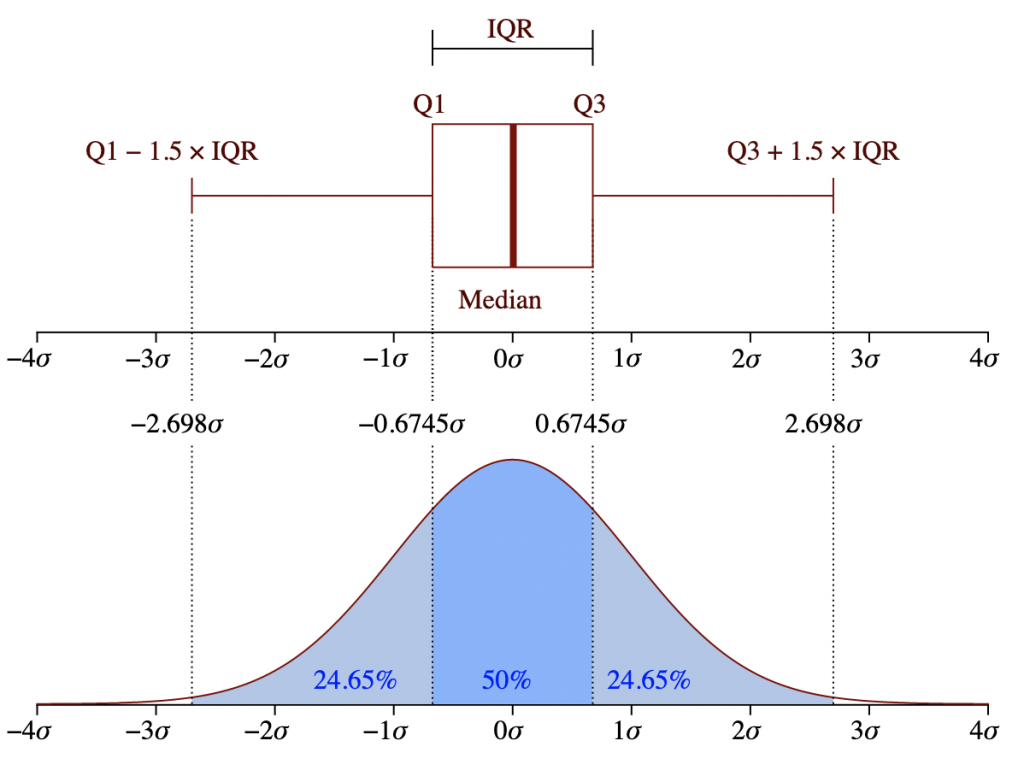
\includegraphics[width=.8\textwidth]{images/IQR.png}
    \caption{Esempio di scarto interquartile in una distribuzione normale \cite{wikipedia:iqr}}
    \label{fig:iqr}
\end{figure}

\subsection{Winsorizing (Percentile Capping)}
Il Winsorizing è un metodo simile al metodo IQR, in questo caso si utilizzano due percentili. Tutti i valori sotto al minimo valore dell'intervallo vengono sostituiti con il minimo, e tutti i valori sopra il massimo valore dell'intervallo vengono sostituiti con il massimo. In questo lavoro sono stati usati due intervalli ($5^{\circ}$ percentile, $95^{\circ}$ percentile) e ($1^{\circ}$ percentile, $99^{\circ}$ percentile).

\noindent
I due intervalli sono stati denominati Winsorizing 90\% e Winsorizing 98\%:
\begin{itemize}
    \item Winsorizing 90\% indica che il 5\% inferiore dei dati viene sostituito con il $5^{\circ}$ percentile e il 5\% superiore dei dati viene sostituito con il $95^{\circ}$ percentile.
    \item Winsorizing 98\% indica che l'1\% inferiore dei dati viene sostituito con il $1^{\circ}$ percentile e l'1\% superiore dei dati viene sostituito con il $99^{\circ}$ percentile.
\end{itemize}

\newpage

\subsubsection{Metodo Scelto}
Per decidere il metodo da usare sono stati utilizzati i boxplot. Sono state confrontate le variabili con i valori assunti dopo l'applicazione dei metodi di rimozione degli outlier (IQR, Winsorizing 90\% e Winsorizing 98\%). Sopra a ogni boxplot sono stati riportati i valori divisi per qualità (good, bad) per visualizzare le quantità di outlier per classe. %\ref{}.

\vspace{4mm}
\noindent
Nonostante il dataset sia sbilanciato, si è deciso di rimuovere completamente gli outlier poiché il numero di outliers risulta molto piccolo (circa il 3\% del training set [\ref{fig:iqr-removed-outliers}].

\vspace{4mm}
\noindent
In seguito sono state confrontate le distribuzioni delle variabili per ogni metodo applicato. 
Il metodo Winsorizing rileva un intervallo di outlier più piccolo e variabile rispetto all'IQR. Inoltre nei casi di distribuzione con distorsione laterale accumula troppi valori agli estremi, alterando così la distribuzione. Con il metodo Winsorizing 98\% si risulta avere una distribuzione più smussata agli estremi. Il metodo IQR non altera la distribuzione, e rimuove un numero non troppo elevato di outliers, quindi si è deciso di usare questo metodo. Per avere un'ulteriore conferma sono stati usati dei Q-Q plot.

\vspace{4mm}
\noindent
I Q-Q (quantile-quantile) plot sono dei grafici utili per capire se due insiemi di dati hanno la stessa distribuzione. Vengono rappresentati i punti in un piano cartesiano attraverso una coppia di quantili. Inoltre viene tracciata una retta a 45° in modo da evidenziare i punti più vicini alla retta. Due insiemi di dati hanno una distribuzione simile se i punti cadono approssimativamente sulla linea di riferimento.
Analizzando i grafici si è visto che il metodo IQR ha valori più vicini alla retta, quindi si è scelto di utilizzare questo.

\newpage
\noindent
Nelle seguenti tabelle sono stati riportati le varie statistiche descrittive delle variabili prima e dopo la rimozione degli outlier con il metodo scelto, nelle tabelle sottostanti notiamo come rimuovendo gli outliers otteniamo un miglioramento di skew, kurtosis e della deviazione standard, mentre le altre statistiche restano praticamente invariate.

\begin{table}[H]
\centering
\resizebox{\linewidth}{!}{
\begin{tabular}[t]{lrrrrrrrr}
\toprule
  & vars & mean & sd & median & min & max & skew & kurtosis\\
\midrule
\cellcolor{gray!6}{fixed.acidity} & \cellcolor{gray!6}{1} & \cellcolor{gray!6}{8.34} & \cellcolor{gray!6}{1.78} & \cellcolor{gray!6}{7.90} & \cellcolor{gray!6}{4.70} & \cellcolor{gray!6}{15.90} & \cellcolor{gray!6}{0.98} & \cellcolor{gray!6}{1.13}\\
volatile.acidity & 2 & 0.53 & 0.18 & 0.52 & 0.12 & 1.58 & 0.71 & 1.46\\
\cellcolor{gray!6}{citric.acid} & \cellcolor{gray!6}{3} & \cellcolor{gray!6}{0.27} & \cellcolor{gray!6}{0.19} & \cellcolor{gray!6}{0.26} & \cellcolor{gray!6}{0.00} & \cellcolor{gray!6}{1.00} & \cellcolor{gray!6}{0.32} & \cellcolor{gray!6}{-0.79}\\
residual.sugar & 4 & 2.53 & 1.40 & 2.20 & 0.90 & 15.40 & 4.47 & 27.53\\
\cellcolor{gray!6}{chlorides} & \cellcolor{gray!6}{5} & \cellcolor{gray!6}{0.09} & \cellcolor{gray!6}{0.05} & \cellcolor{gray!6}{0.08} & \cellcolor{gray!6}{0.01} & \cellcolor{gray!6}{0.61} & \cellcolor{gray!6}{5.89} & \cellcolor{gray!6}{45.36}\\
\addlinespace
free.sulfur.dioxide & 6 & 15.79 & 10.58 & 13.00 & 1.00 & 72.00 & 1.29 & 2.19\\
\cellcolor{gray!6}{total.sulfur.dioxide} & \cellcolor{gray!6}{7} & \cellcolor{gray!6}{45.23} & \cellcolor{gray!6}{31.87} & \cellcolor{gray!6}{37.00} & \cellcolor{gray!6}{6.00} & \cellcolor{gray!6}{278.00} & \cellcolor{gray!6}{1.41} & \cellcolor{gray!6}{2.87}\\
density & 8 & 1.00 & 0.00 & 1.00 & 0.99 & 1.00 & 0.05 & 0.90\\
\cellcolor{gray!6}{pH} & \cellcolor{gray!6}{9} & \cellcolor{gray!6}{3.31} & \cellcolor{gray!6}{0.15} & \cellcolor{gray!6}{3.31} & \cellcolor{gray!6}{2.74} & \cellcolor{gray!6}{4.01} & \cellcolor{gray!6}{0.11} & \cellcolor{gray!6}{0.62}\\
sulphates & 10 & 0.66 & 0.17 & 0.62 & 0.33 & 2.00 & 2.57 & 13.02\\
\addlinespace
\cellcolor{gray!6}{alcohol} & \cellcolor{gray!6}{11} & \cellcolor{gray!6}{10.45} & \cellcolor{gray!6}{1.07} & \cellcolor{gray!6}{10.20} & \cellcolor{gray!6}{8.40} & \cellcolor{gray!6}{14.90} & \cellcolor{gray!6}{0.84} & \cellcolor{gray!6}{0.13}\\
\bottomrule
\end{tabular}}
\caption{Prima della rimozione}
\end{table}


\begin{table}
\centering
\resizebox{\linewidth}{!}{
\begin{tabular}[t]{lrrrrrrrr}
\toprule
  & vars & mean & sd & median & min & max & skew & kurtosis\\
\midrule
\cellcolor{gray!6}{fixed.acidity} & \cellcolor{gray!6}{1} & \cellcolor{gray!6}{6.83} & \cellcolor{gray!6}{0.77} & \cellcolor{gray!6}{6.80} & \cellcolor{gray!6}{4.70} & \cellcolor{gray!6}{9.00} & \cellcolor{gray!6}{0.22} & \cellcolor{gray!6}{0.02}\\
volatile.acidity & 2 & 0.27 & 0.08 & 0.26 & 0.08 & 0.48 & 0.41 & -0.23\\
\cellcolor{gray!6}{citric.acid} & \cellcolor{gray!6}{3} & \cellcolor{gray!6}{0.32} & \cellcolor{gray!6}{0.09} & \cellcolor{gray!6}{0.31} & \cellcolor{gray!6}{0.10} & \cellcolor{gray!6}{0.57} & \cellcolor{gray!6}{0.41} & \cellcolor{gray!6}{-0.02}\\
residual.sugar & 4 & 6.39 & 4.96 & 5.20 & 0.60 & 22.00 & 0.73 & -0.52\\
\cellcolor{gray!6}{chlorides} & \cellcolor{gray!6}{5} & \cellcolor{gray!6}{0.04} & \cellcolor{gray!6}{0.01} & \cellcolor{gray!6}{0.04} & \cellcolor{gray!6}{0.02} & \cellcolor{gray!6}{0.07} & \cellcolor{gray!6}{0.10} & \cellcolor{gray!6}{-0.25}\\
\addlinespace
free.sulfur.dioxide & 6 & 34.53 & 15.28 & 33.00 & 2.00 & 78.00 & 0.32 & -0.45\\
\cellcolor{gray!6}{total.sulfur.dioxide} & \cellcolor{gray!6}{7} & \cellcolor{gray!6}{138.24} & \cellcolor{gray!6}{41.26} & \cellcolor{gray!6}{135.00} & \cellcolor{gray!6}{21.00} & \cellcolor{gray!6}{256.00} & \cellcolor{gray!6}{0.23} & \cellcolor{gray!6}{-0.33}\\
density & 8 & 0.99 & 0.00 & 0.99 & 0.99 & 1.00 & 0.23 & -0.78\\
\cellcolor{gray!6}{pH} & \cellcolor{gray!6}{9} & \cellcolor{gray!6}{3.18} & \cellcolor{gray!6}{0.14} & \cellcolor{gray!6}{3.17} & \cellcolor{gray!6}{2.79} & \cellcolor{gray!6}{3.57} & \cellcolor{gray!6}{0.22} & \cellcolor{gray!6}{-0.18}\\
sulphates & 10 & 0.48 & 0.10 & 0.47 & 0.23 & 0.76 & 0.48 & -0.08\\
\addlinespace
\cellcolor{gray!6}{alcohol} & \cellcolor{gray!6}{11} & \cellcolor{gray!6}{10.52} & \cellcolor{gray!6}{1.24} & \cellcolor{gray!6}{10.40} & \cellcolor{gray!6}{8.00} & \cellcolor{gray!6}{14.20} & \cellcolor{gray!6}{0.49} & \cellcolor{gray!6}{-0.69}\\
\bottomrule
\end{tabular}}
\end{table}


\newpage
\noindent
Nel seguente grafico è stato confrontato il numero di outliers rimossi per variabili divisi per classe, attraverso il metodo IQR. La classe minoritaria (good) ha meno outliers come ci si può aspettare. Le variabili con più outliers rilevati sono \textit{residual.sugar}, \textit{chlorides}, \textit{sulfur.dioxide} e \textit{sulphates}. La variabile \textit{citric.acid} ha quasi zero outliers per entrambe le classi. In totale il numero di outliers rilevati e rimossi con il metodo IQR costituiscono il 2.88\% del training set.

\begin{figure}
    \centering
    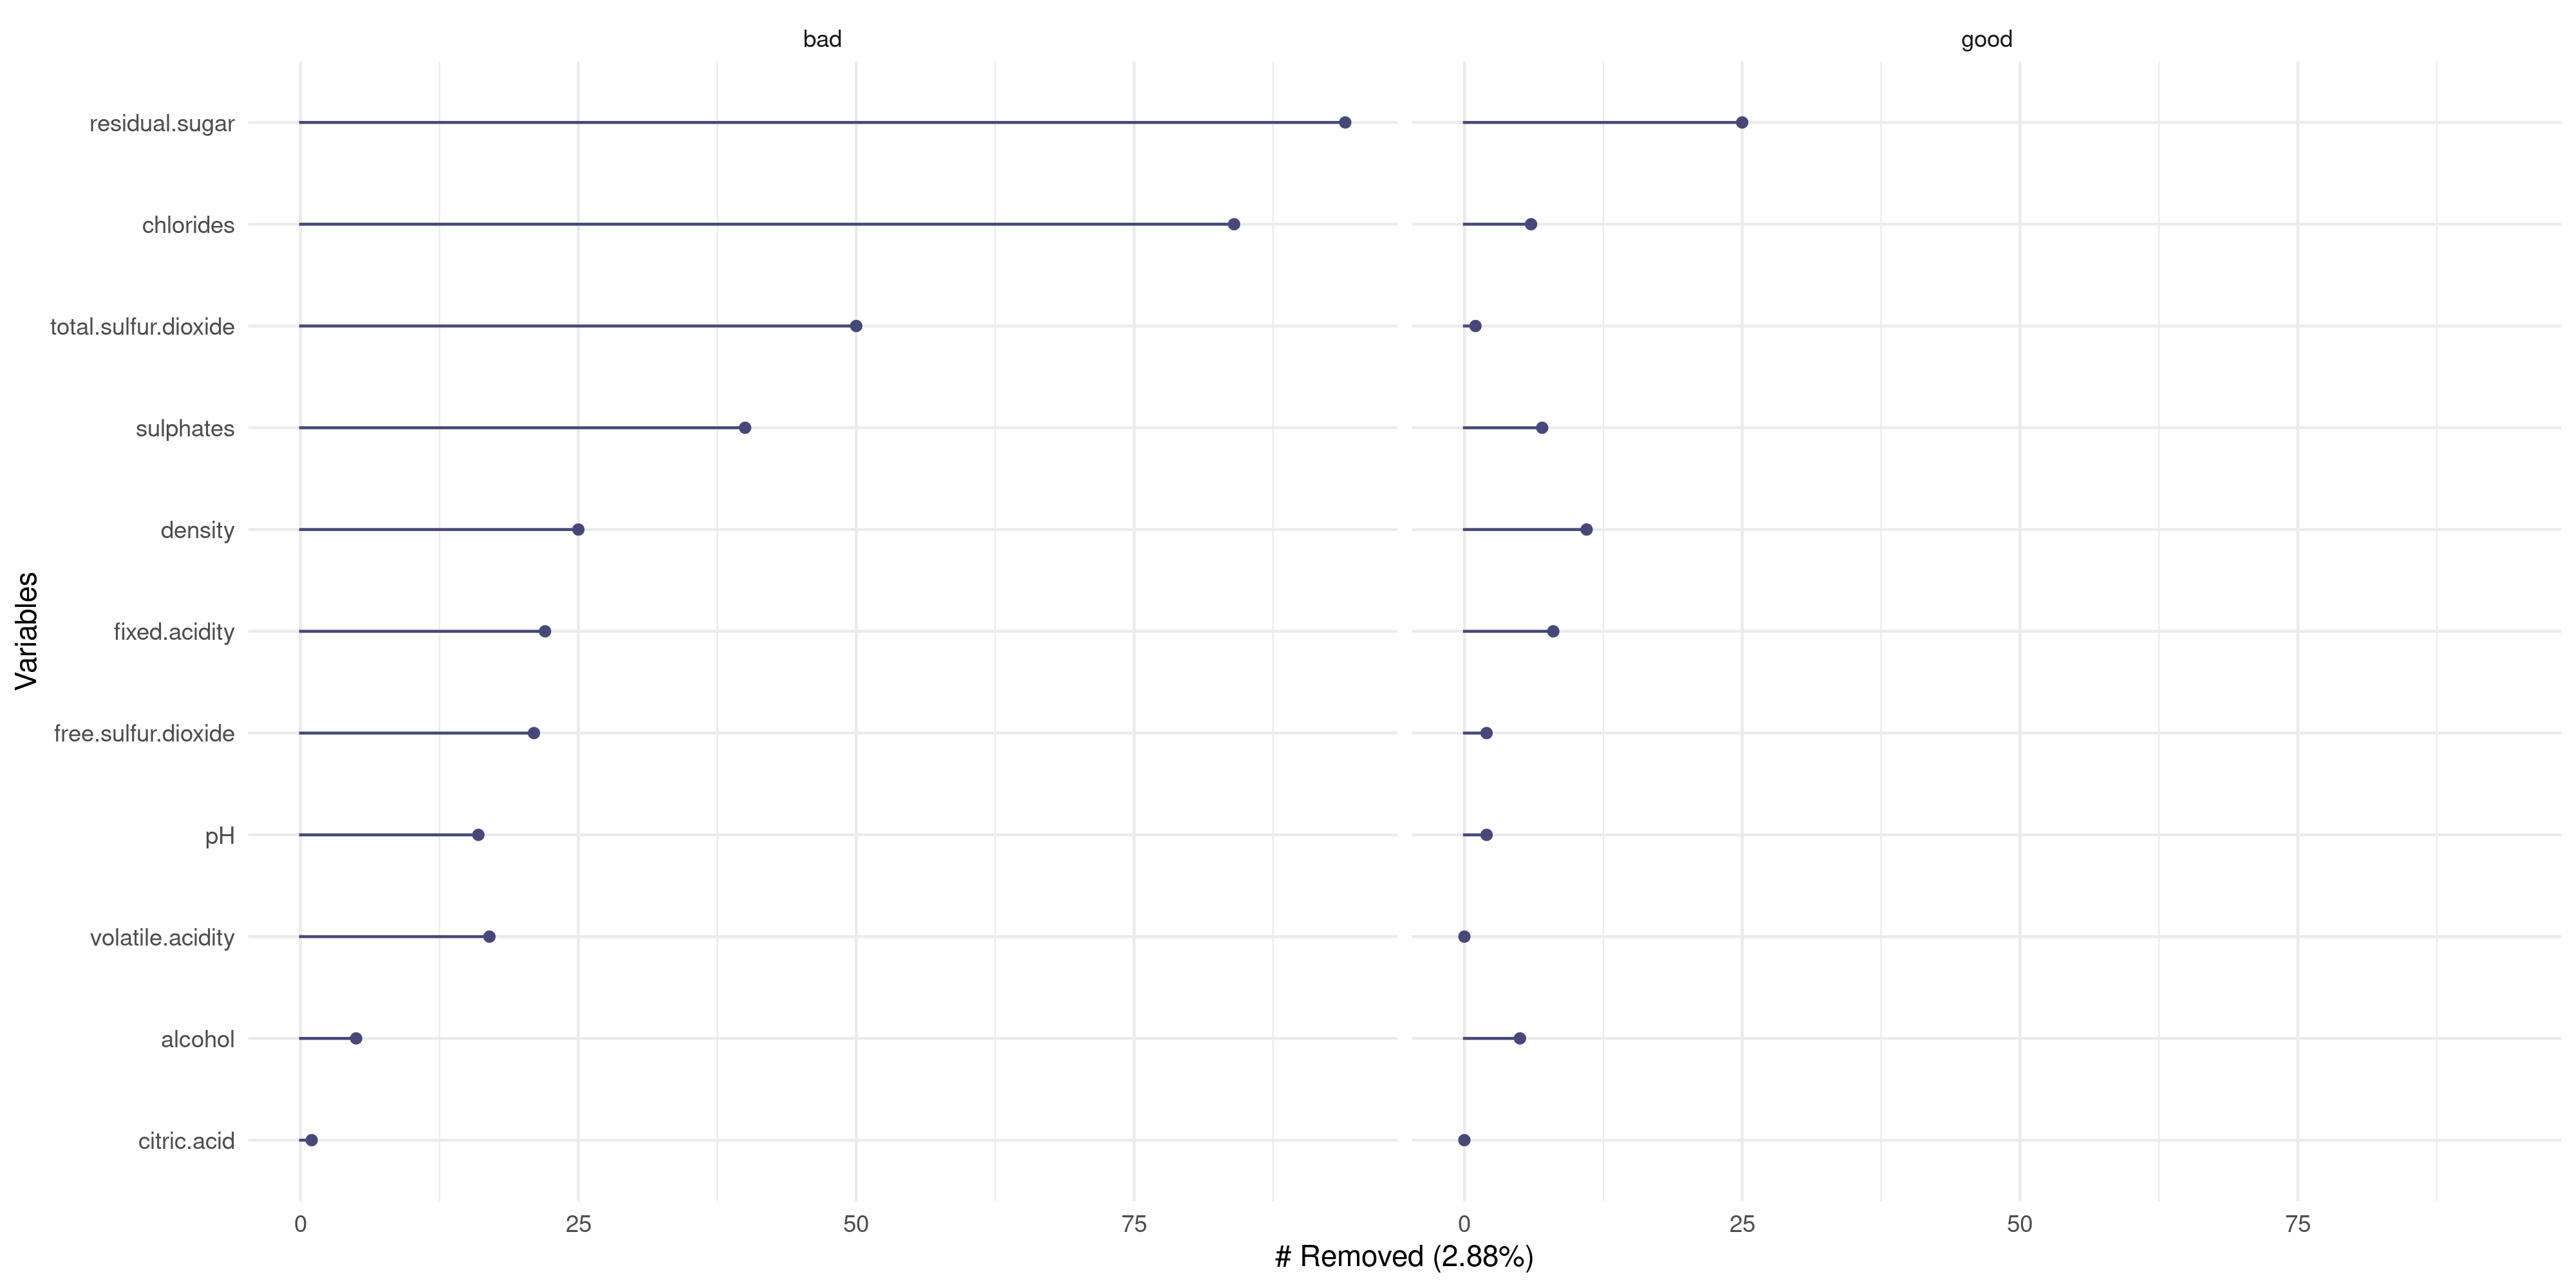
\includegraphics[width=\textwidth]{images/outliers/iqr-outliers.png}
    \caption{Numero di outliers rimossi per ogni variabile divisi per classe}
    \label{fig:iqr-removed-outliers}
\end{figure}

\newpage

\subsection{Grafici}
In questa sezione vengono riportati i grafici che sono stati utilizzati per l'analisi univariata degli outliers. 

\begin{figure}[H]
    \centering

    \subfloat[]{%
        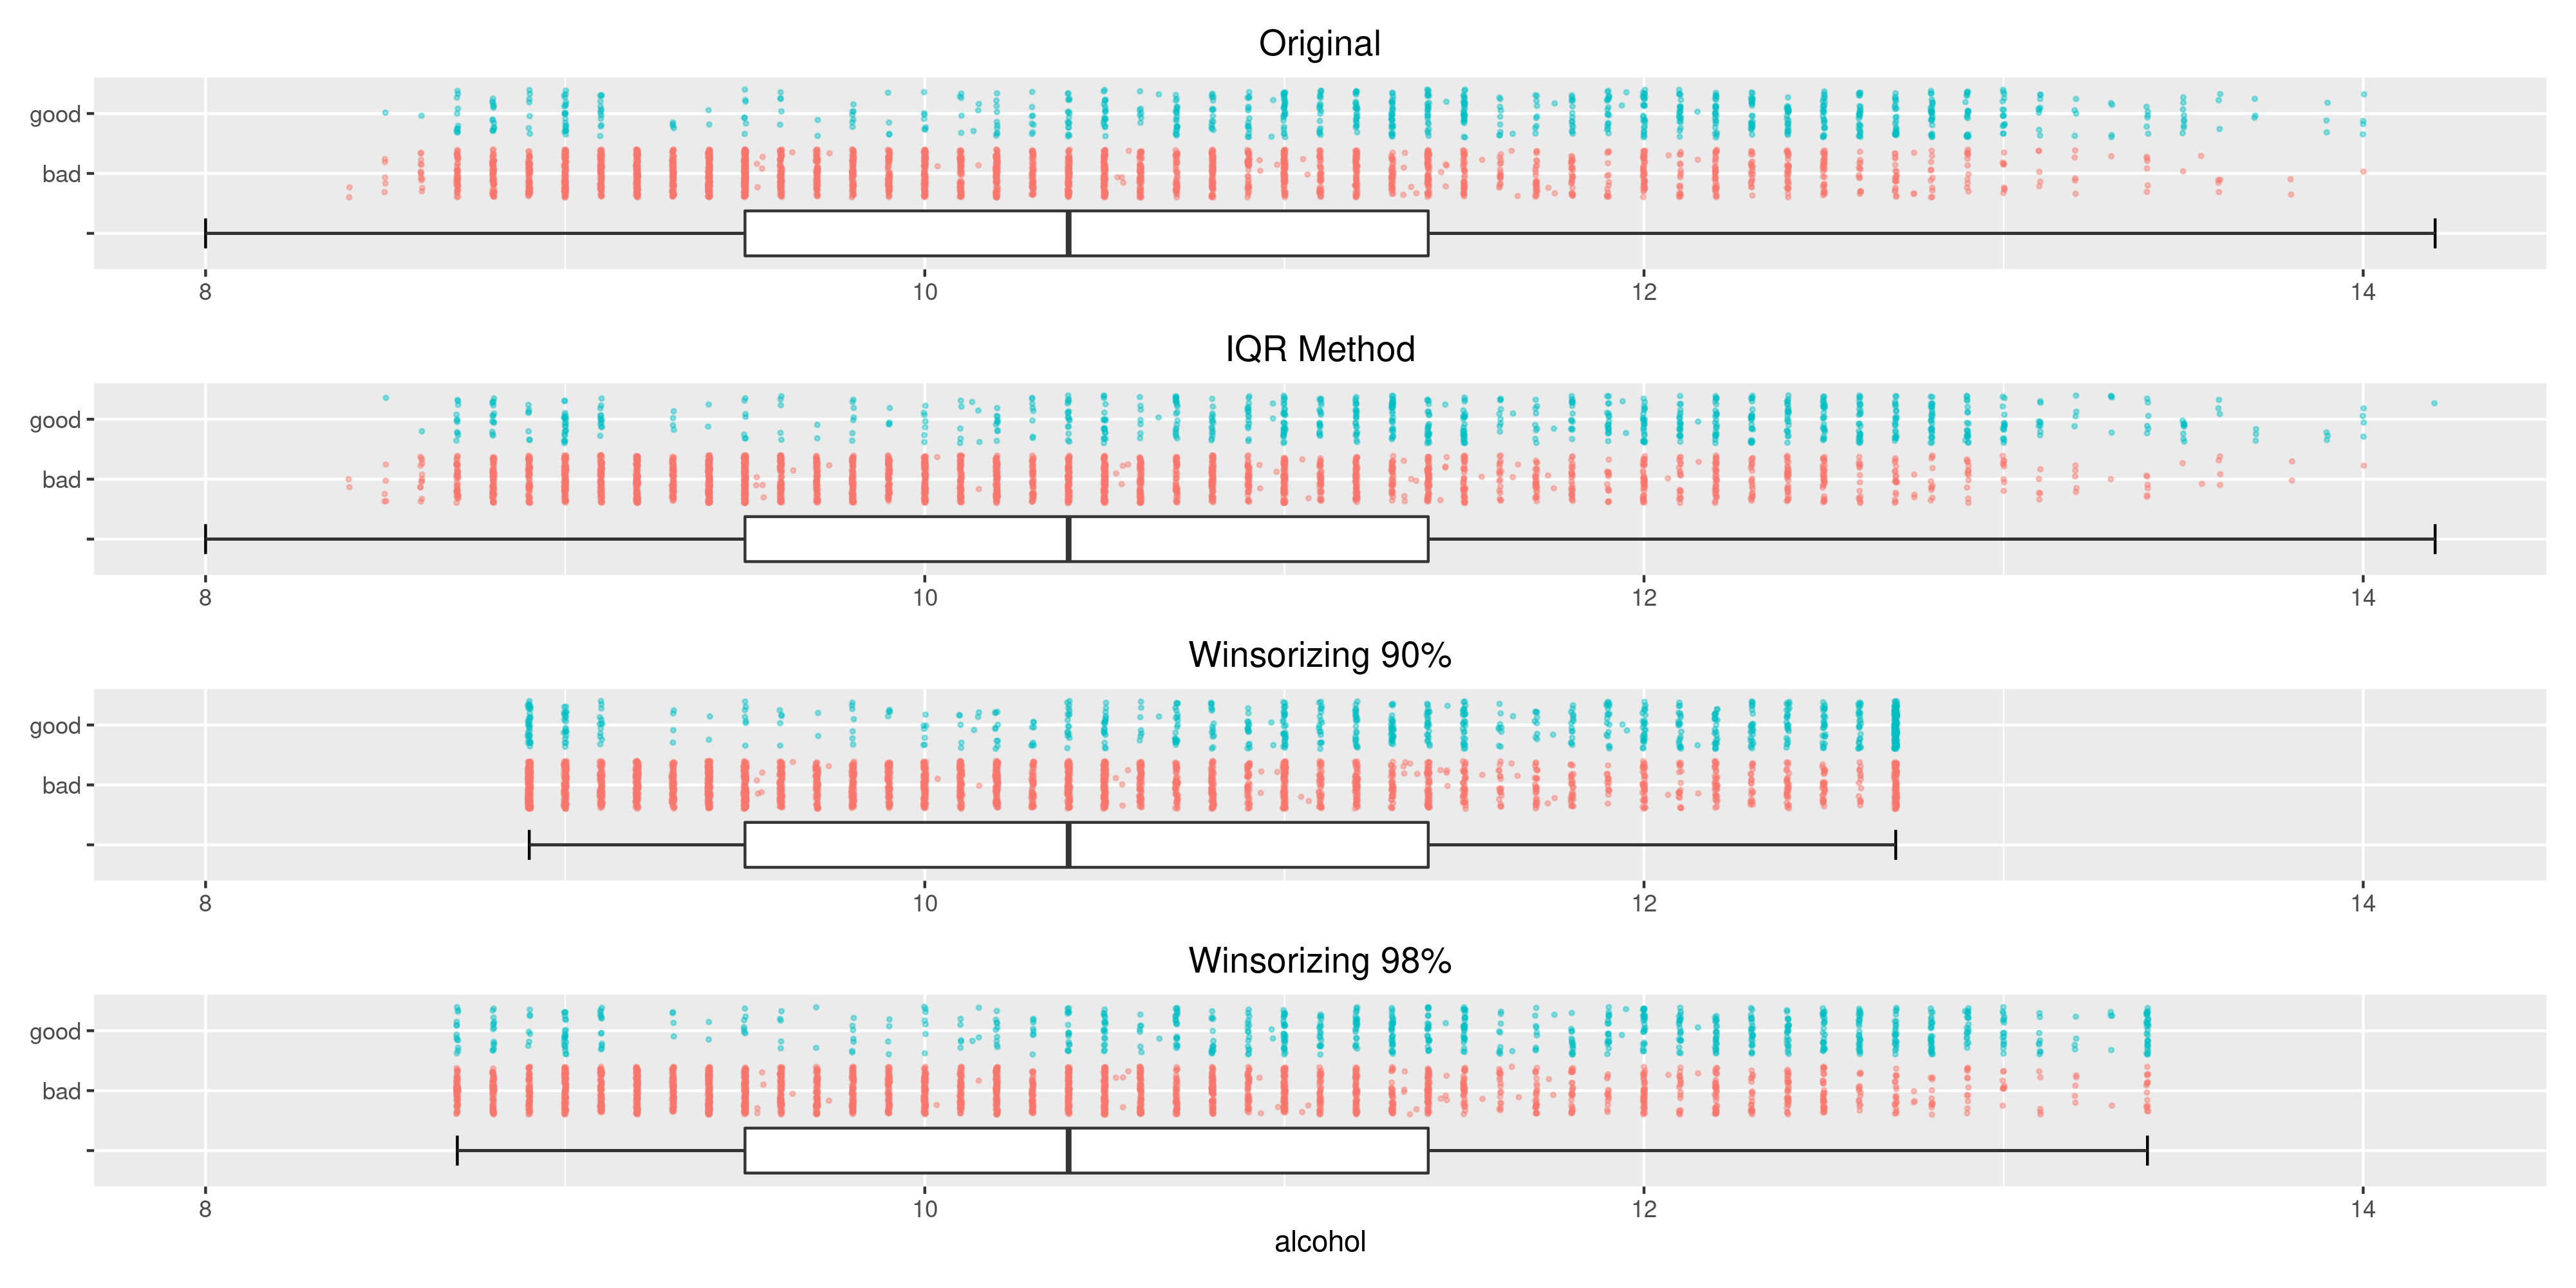
\includegraphics[width=0.99\textwidth]{images/outliers/alcohol_boxplot.png}
    }

    \subfloat[]{%
        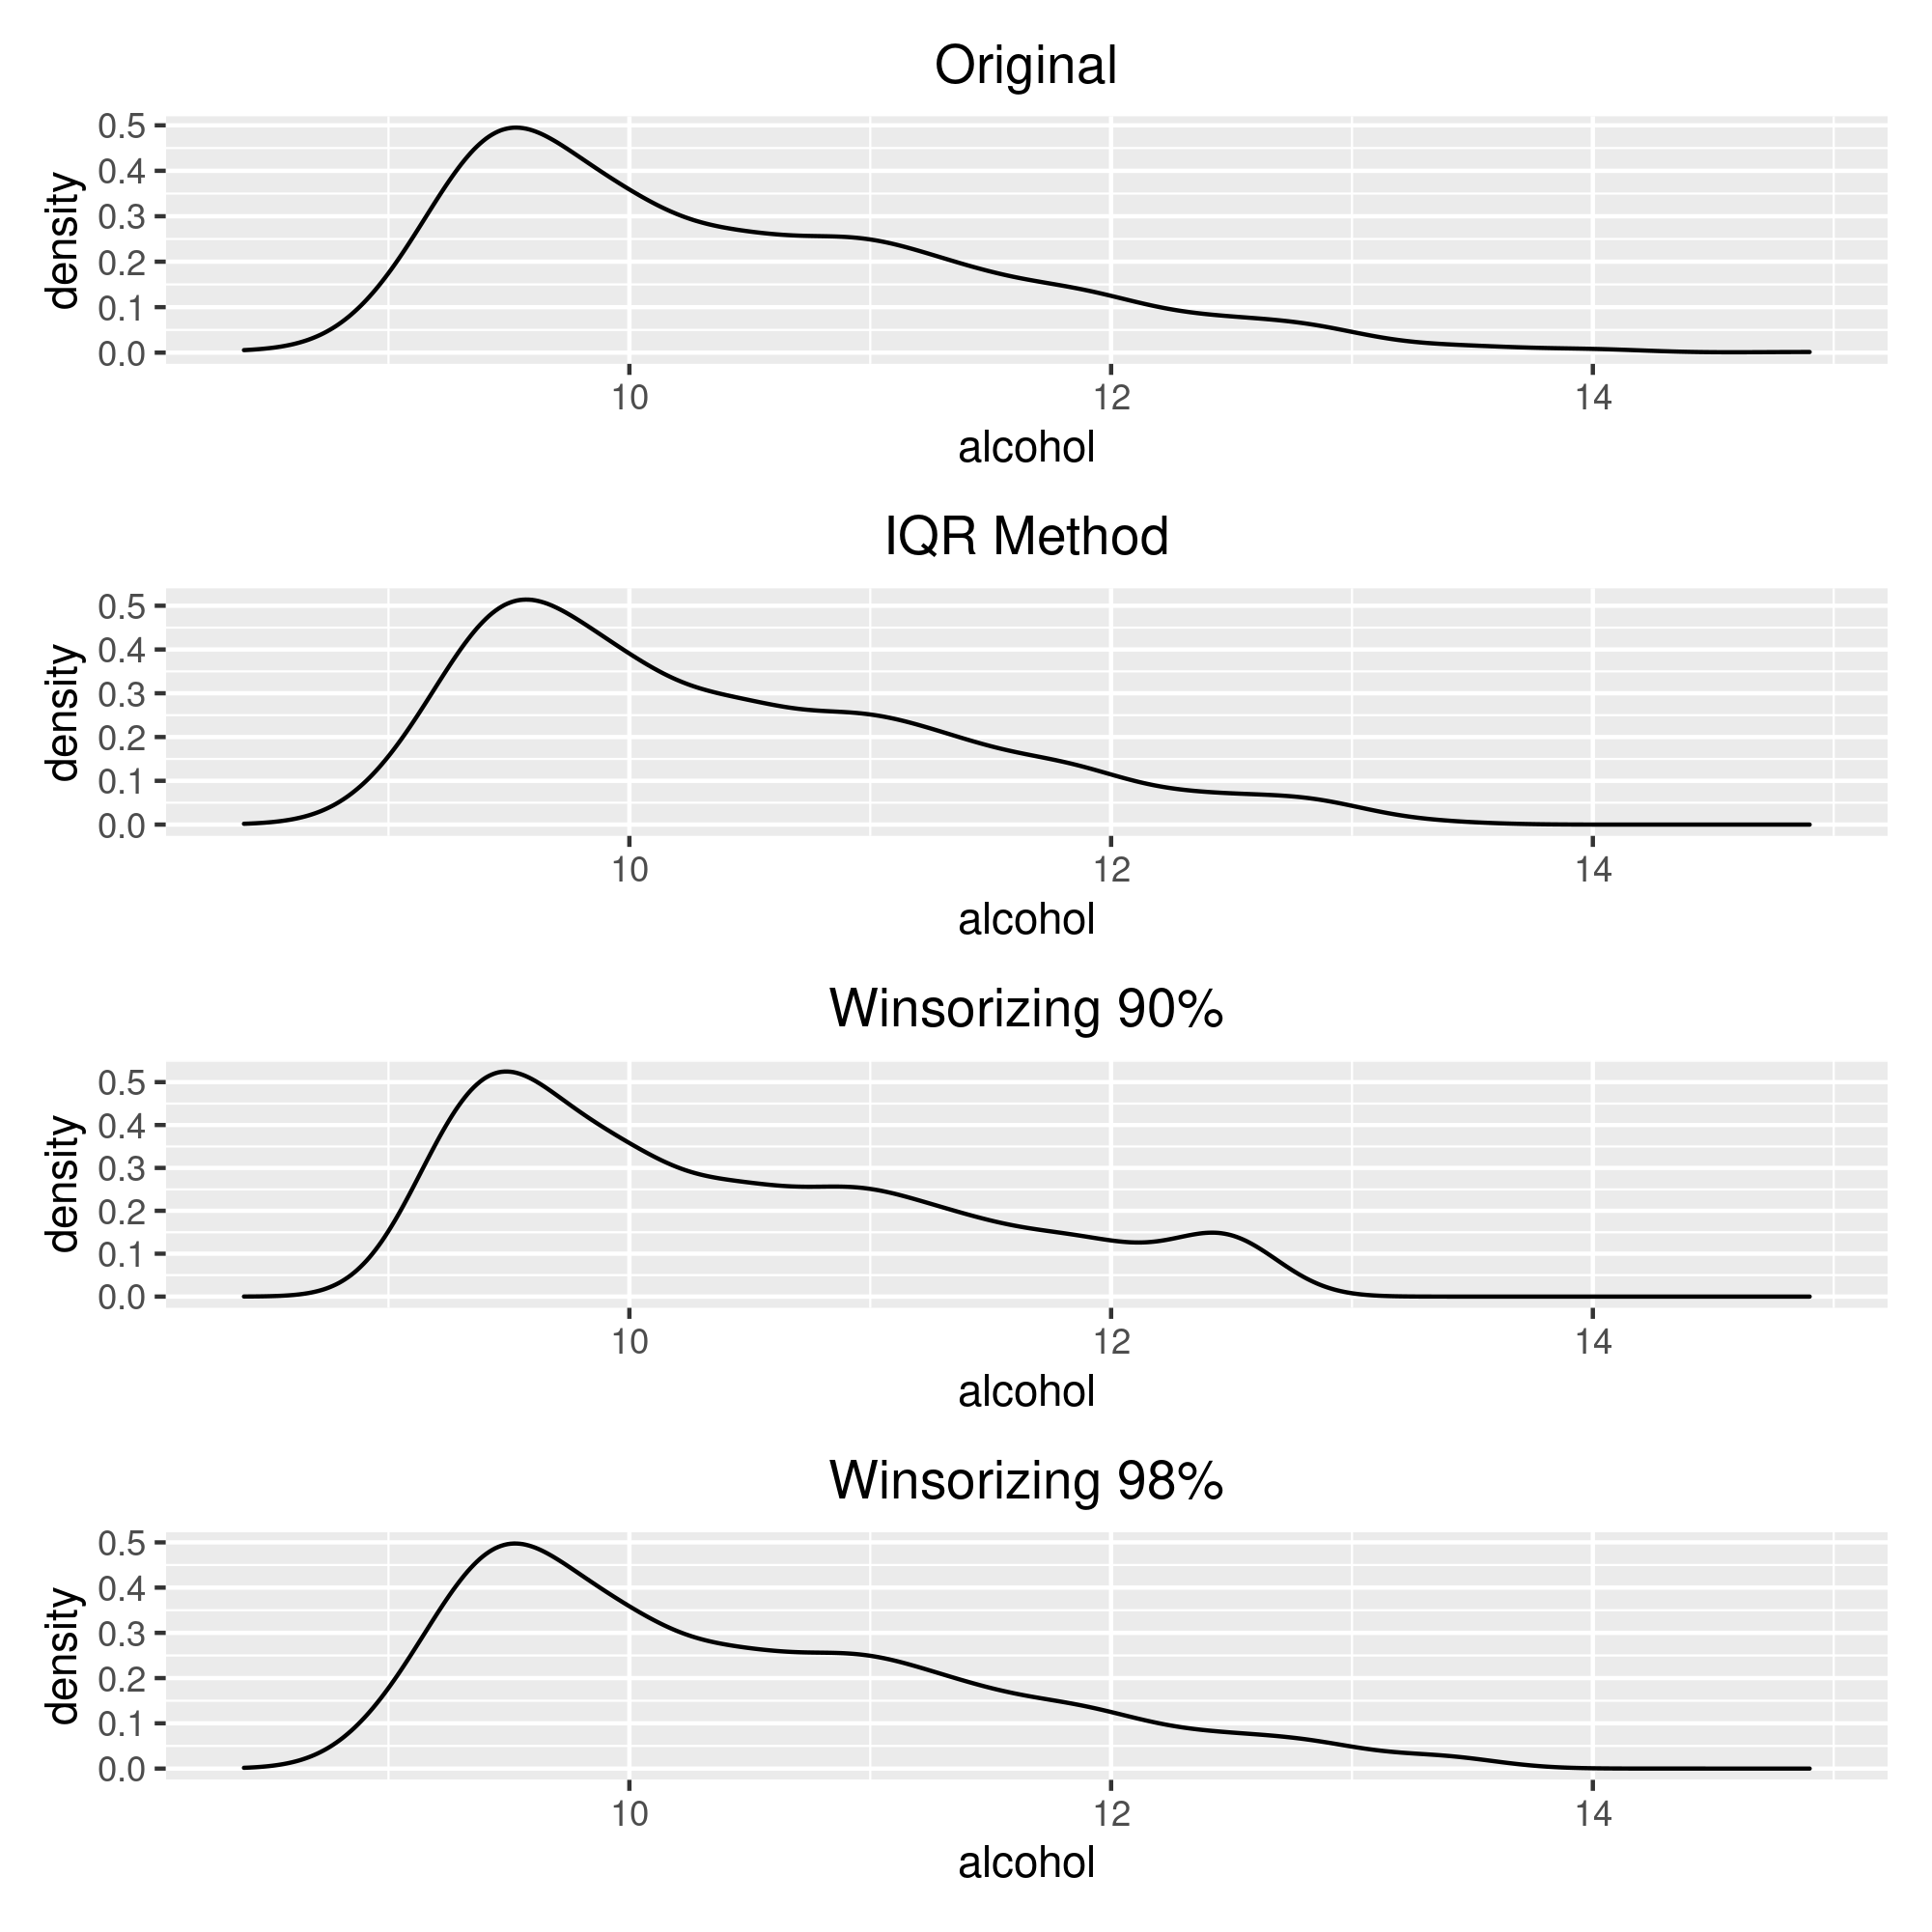
\includegraphics[width=0.45\textwidth]{images/outliers/alcohol_distribution.png}
    }\quad
    \subfloat[]{%
        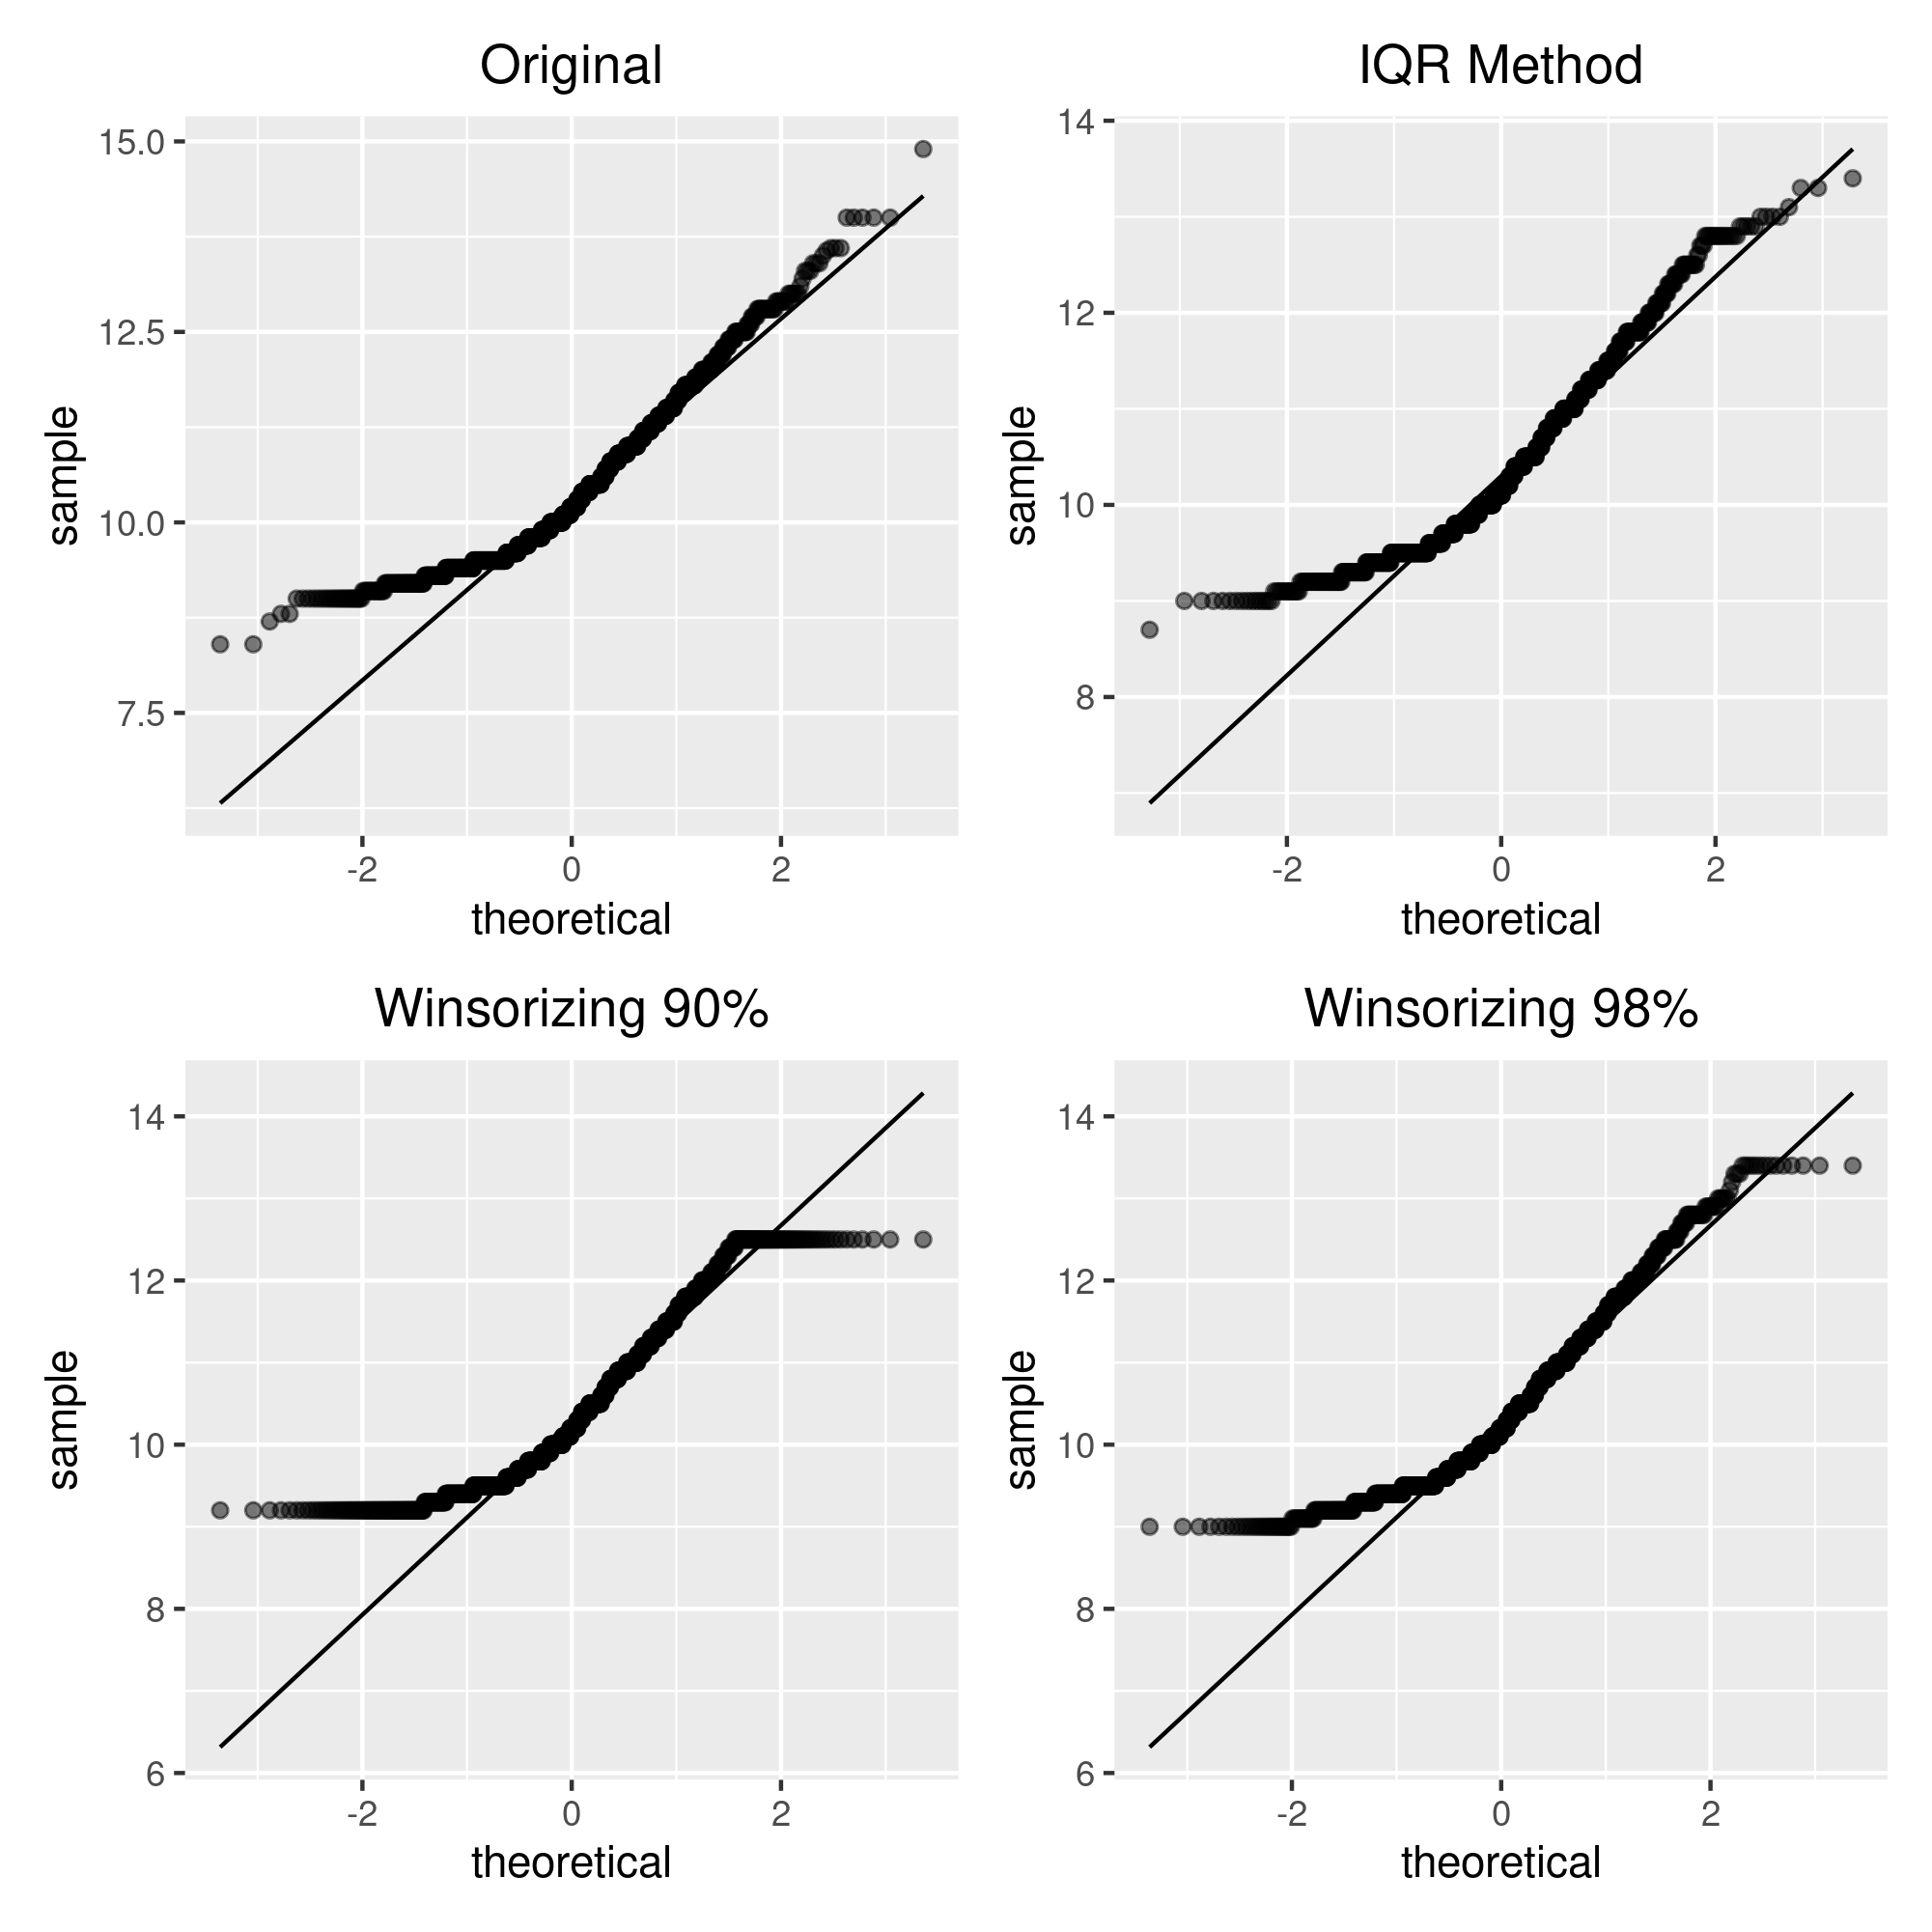
\includegraphics[width=0.45\textwidth]{images/outliers/alcohol_qqplot.png}
    }

    \label{fig:outliers-alcohol}
    \caption{Alcohol}
\end{figure}

\newpage

\begin{figure}[H]
    \centering

    \subfloat[]{%
        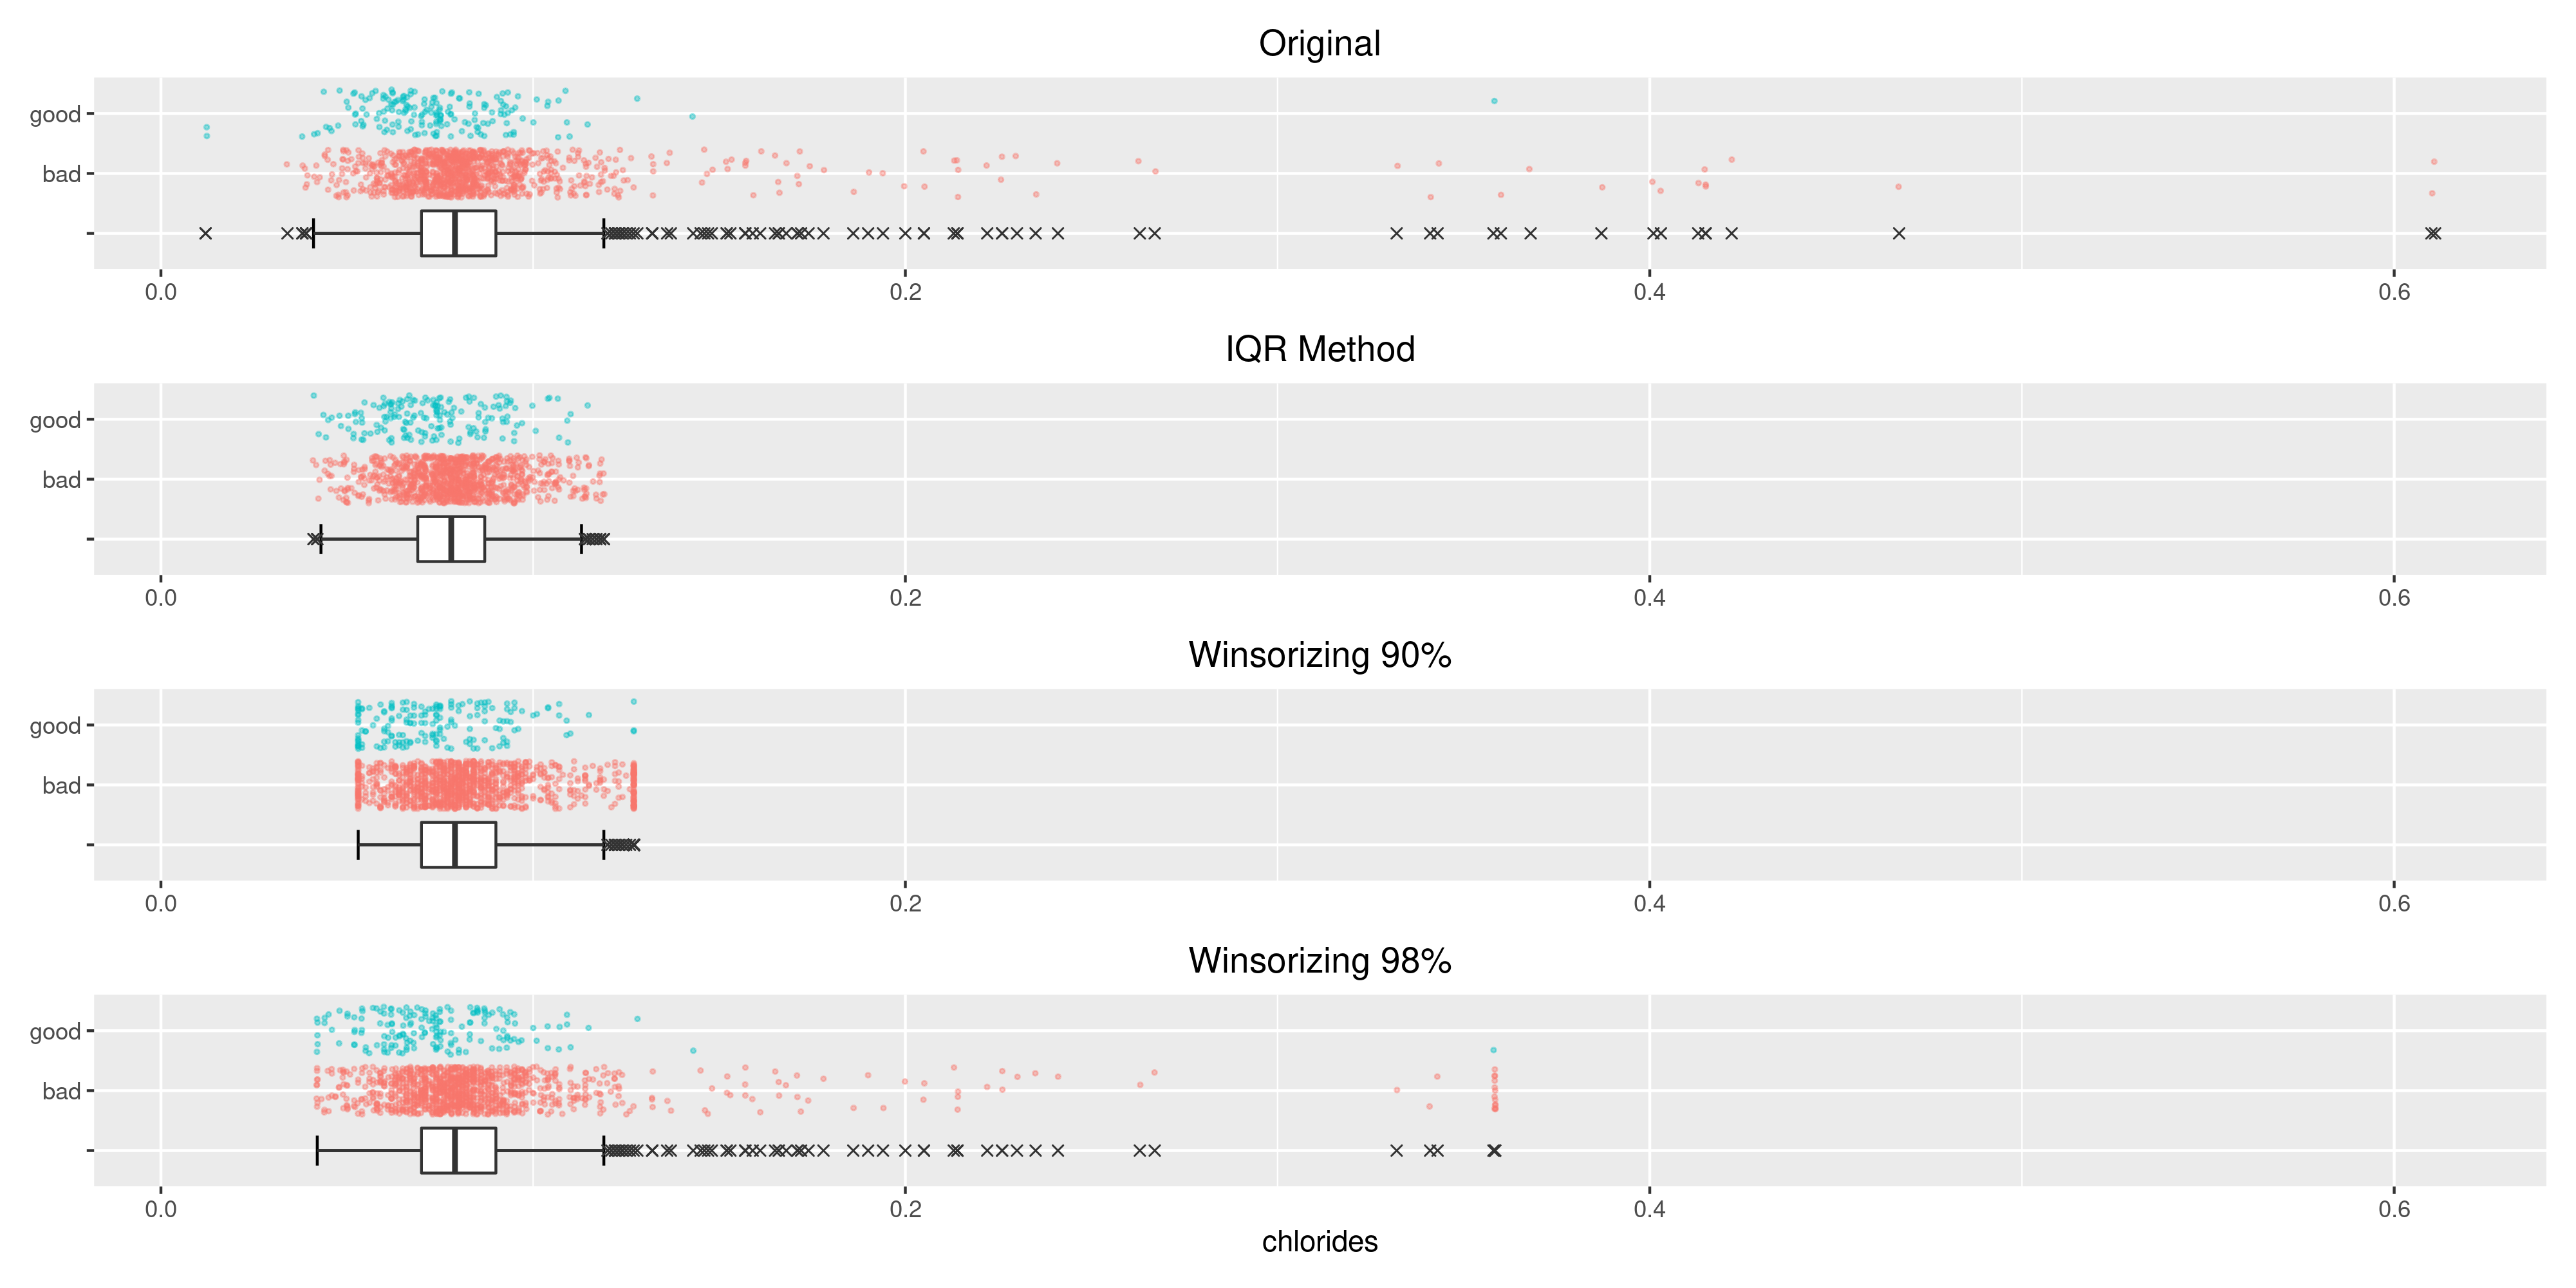
\includegraphics[width=0.99\textwidth]{images/outliers/chlorides_boxplot.png}
    }

    \subfloat[]{%
        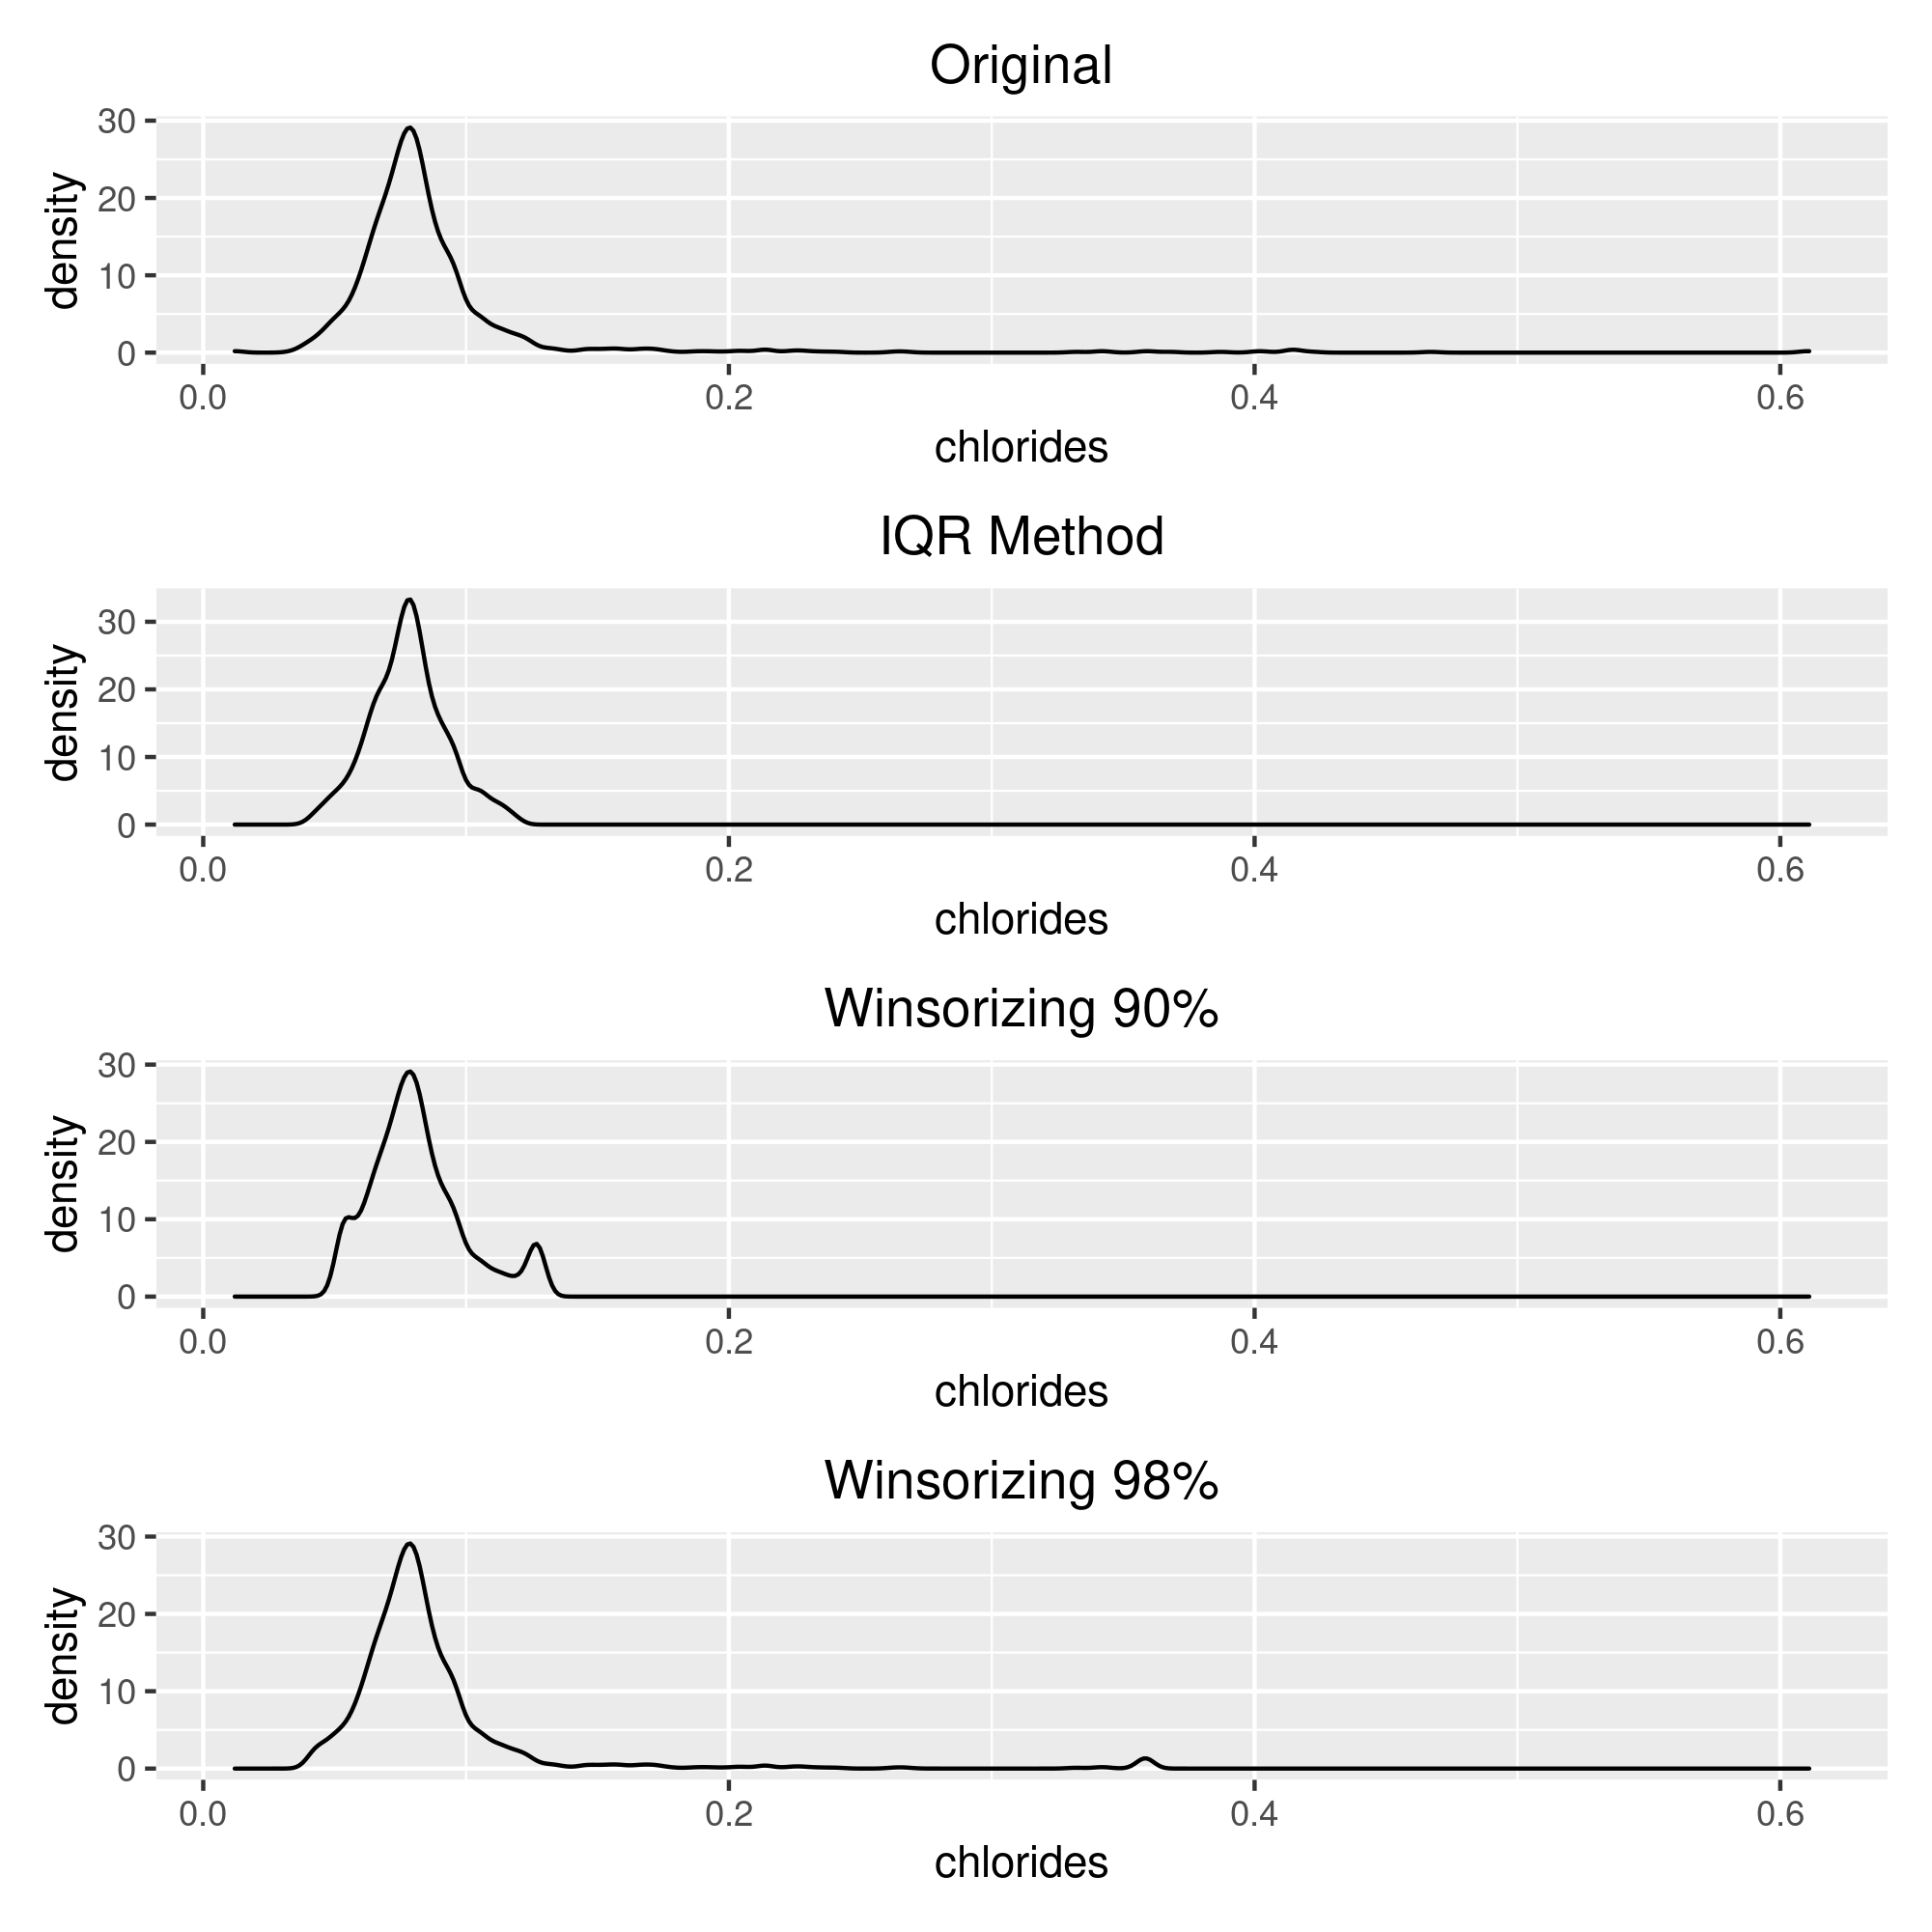
\includegraphics[width=0.45\textwidth]{images/outliers/chlorides_distribution.png}
    }\qquad
    \subfloat[]{%
        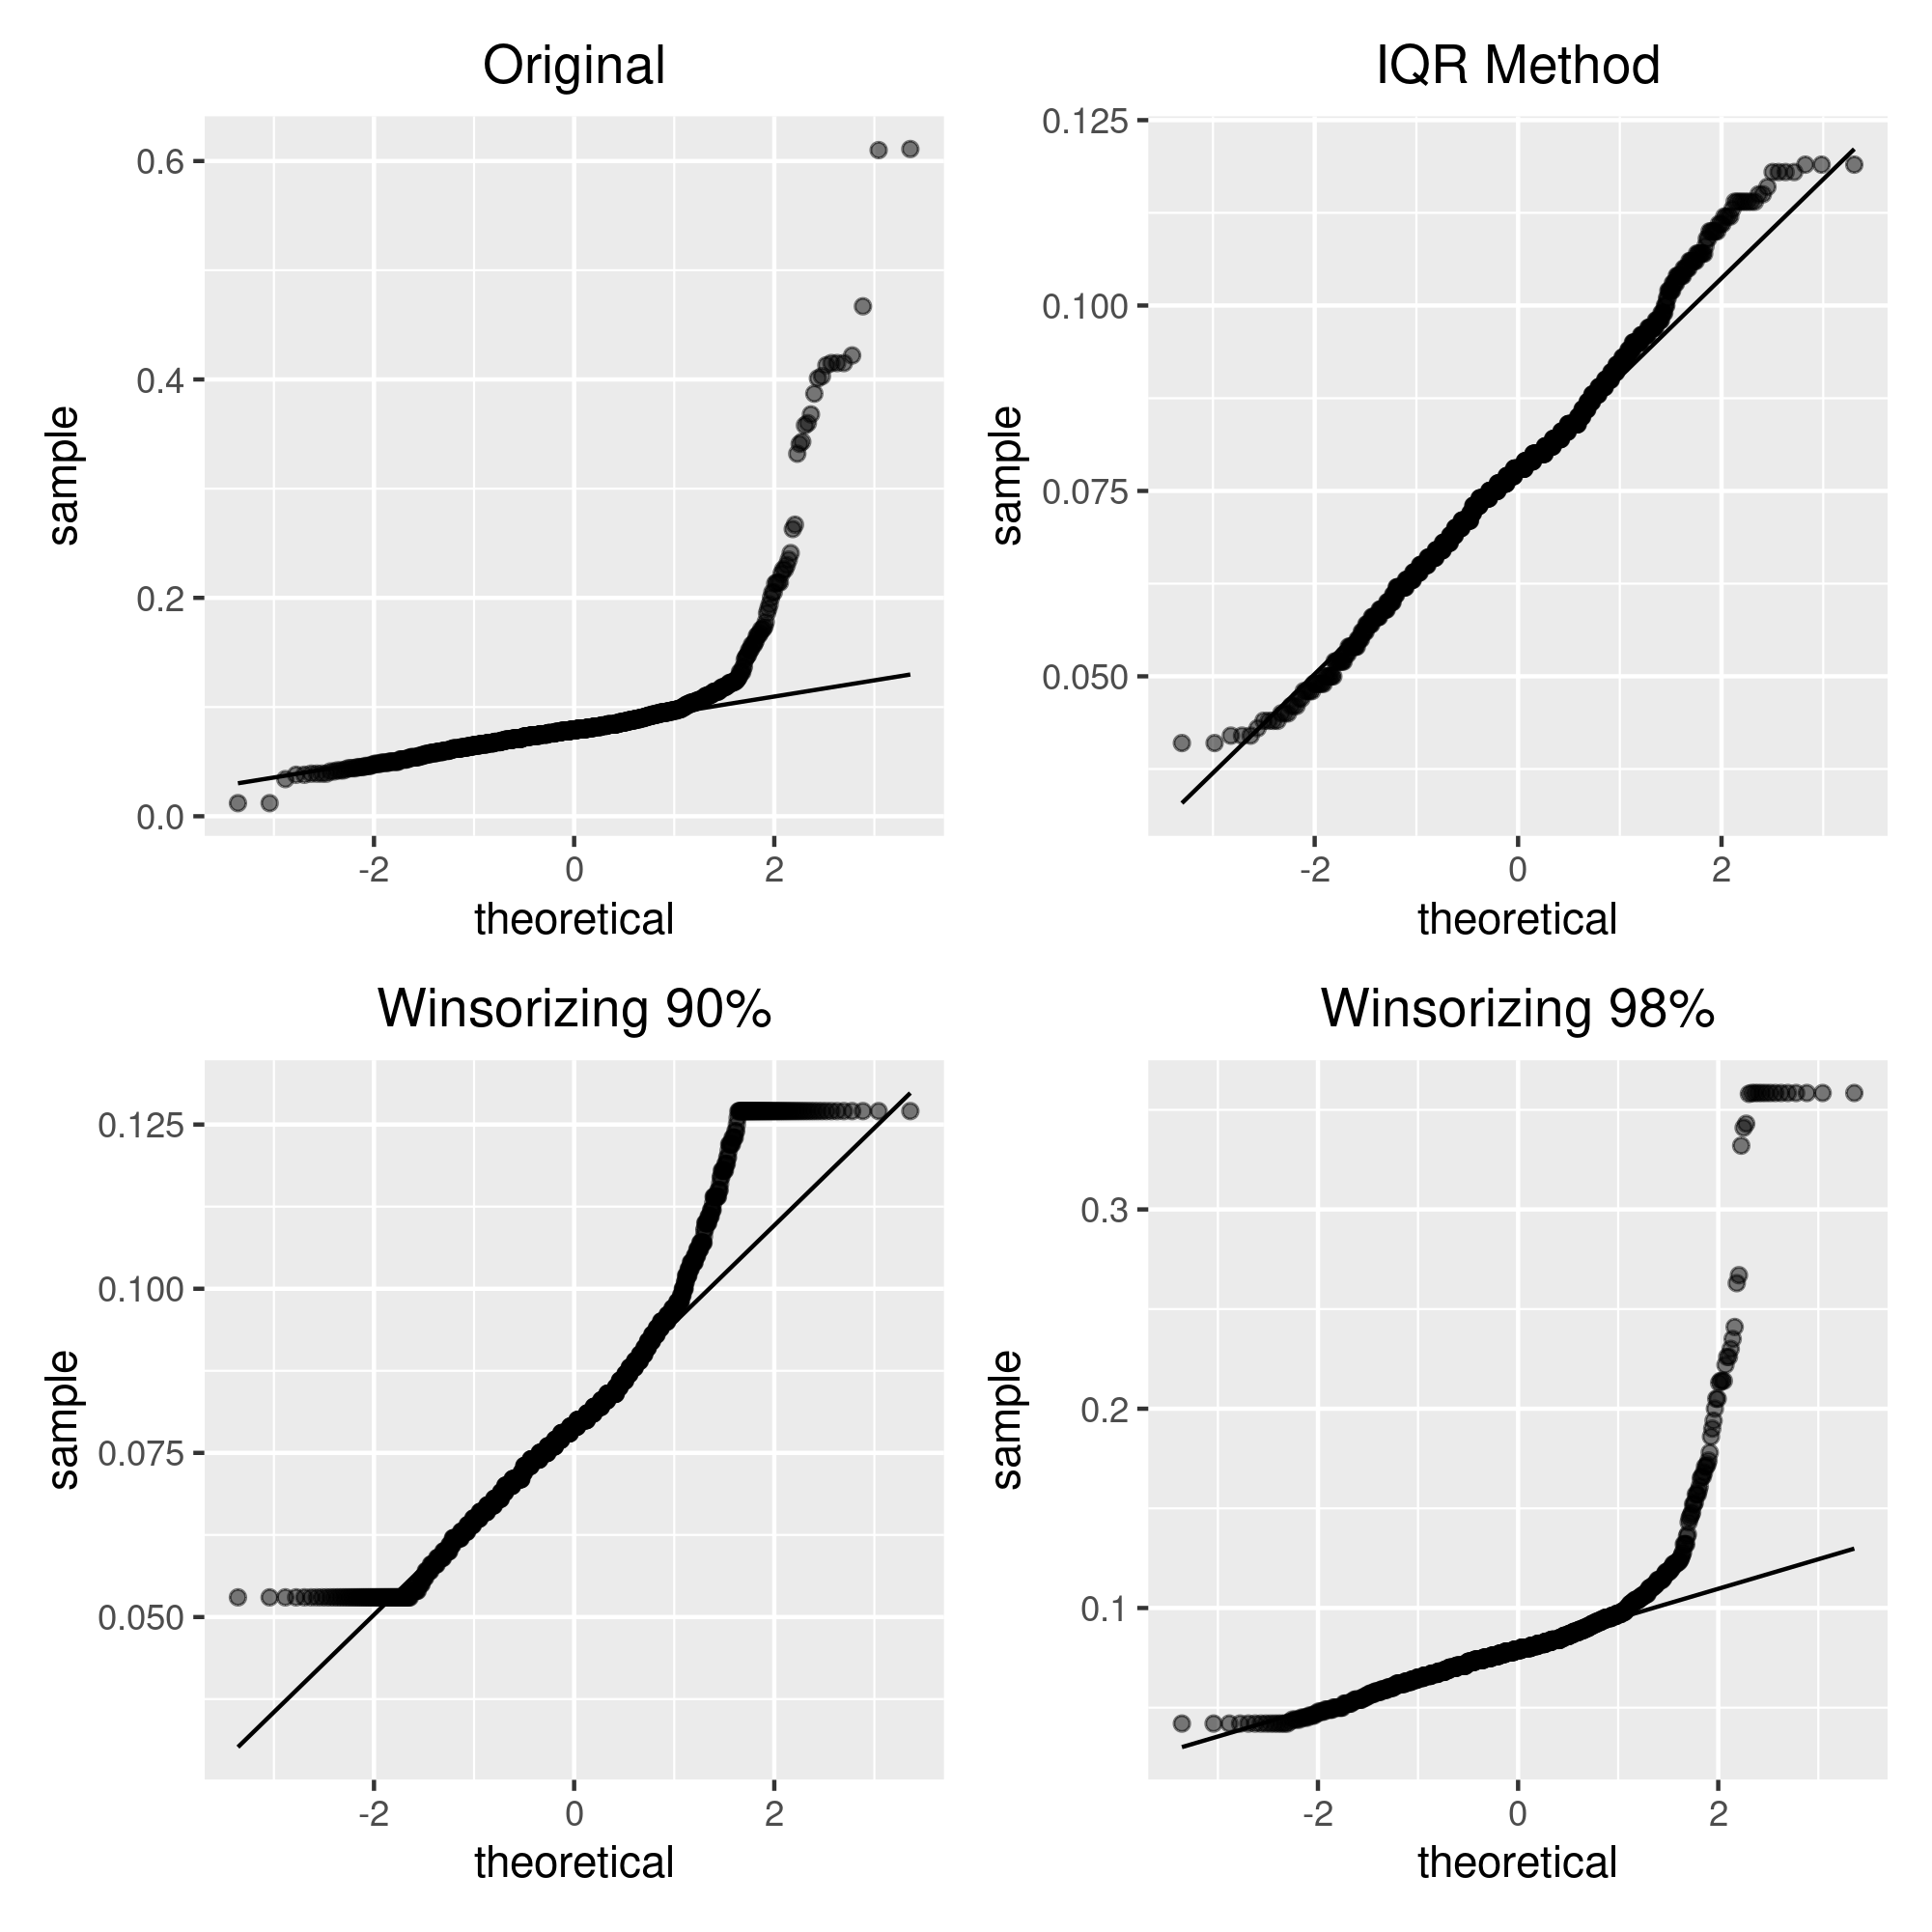
\includegraphics[width=0.45\textwidth]{images/outliers/chlorides_qqplot.png}
    }

    \label{fig:outliers-chlorides}
    \caption{Chlorides}
\end{figure}

\begin{figure}[H]
    \centering

    \subfloat[]{%
        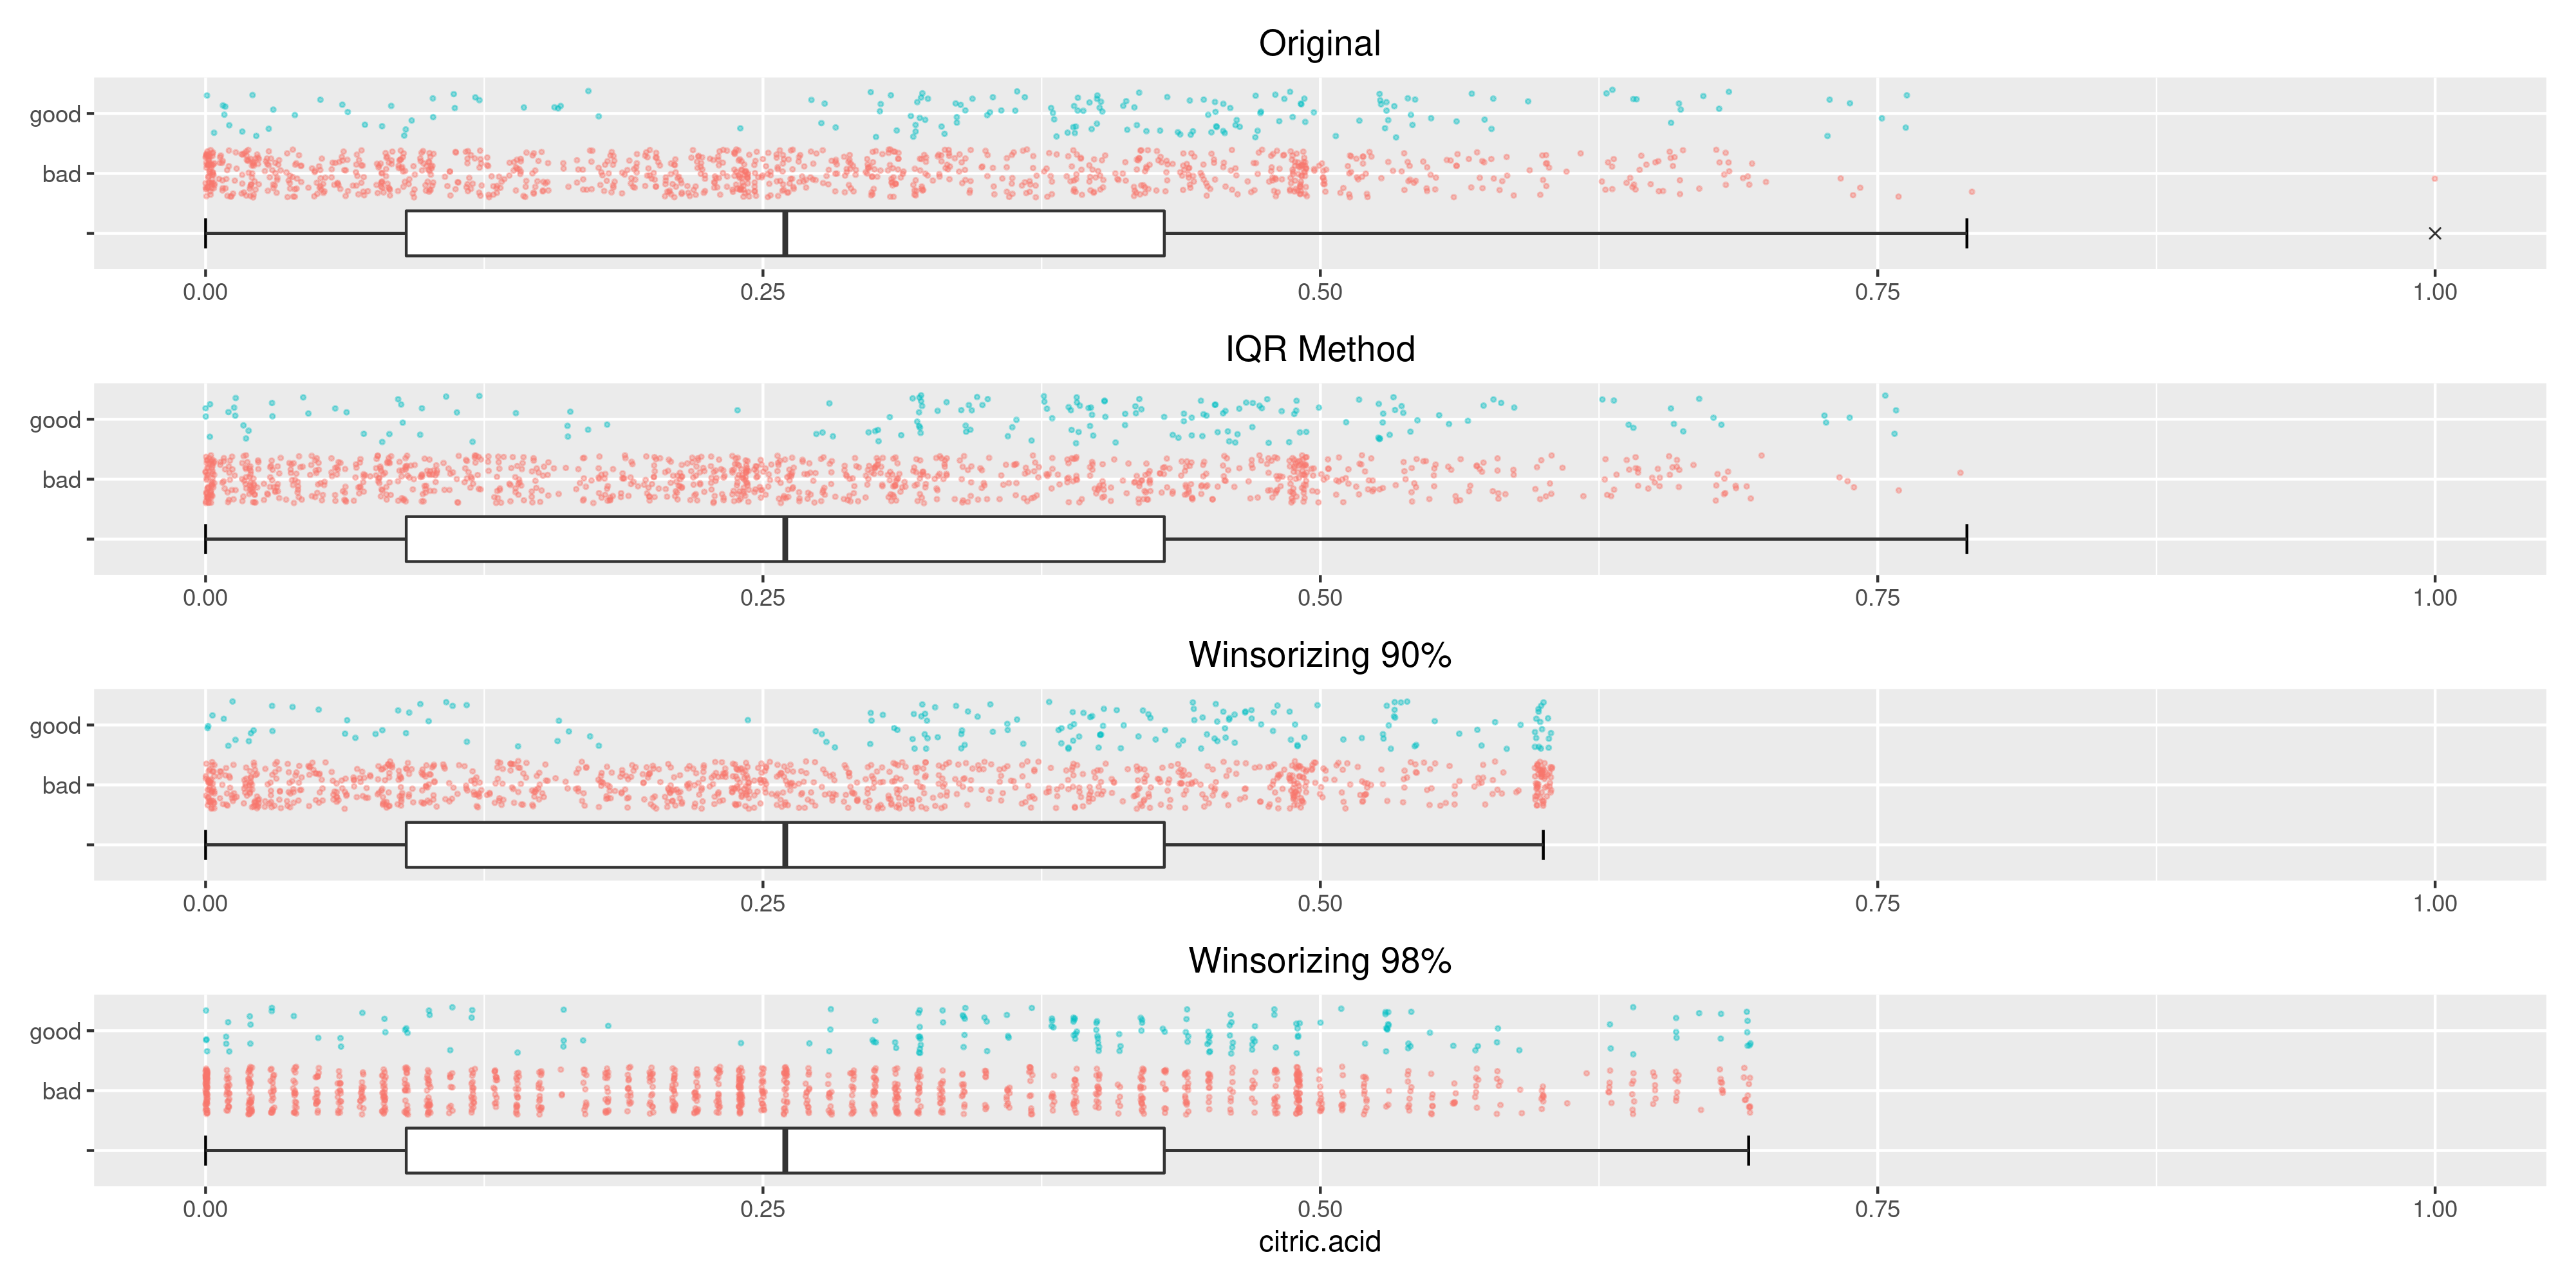
\includegraphics[width=0.99\textwidth]{images/outliers/citric.acid_boxplot.png}
    }

    \subfloat[]{%
        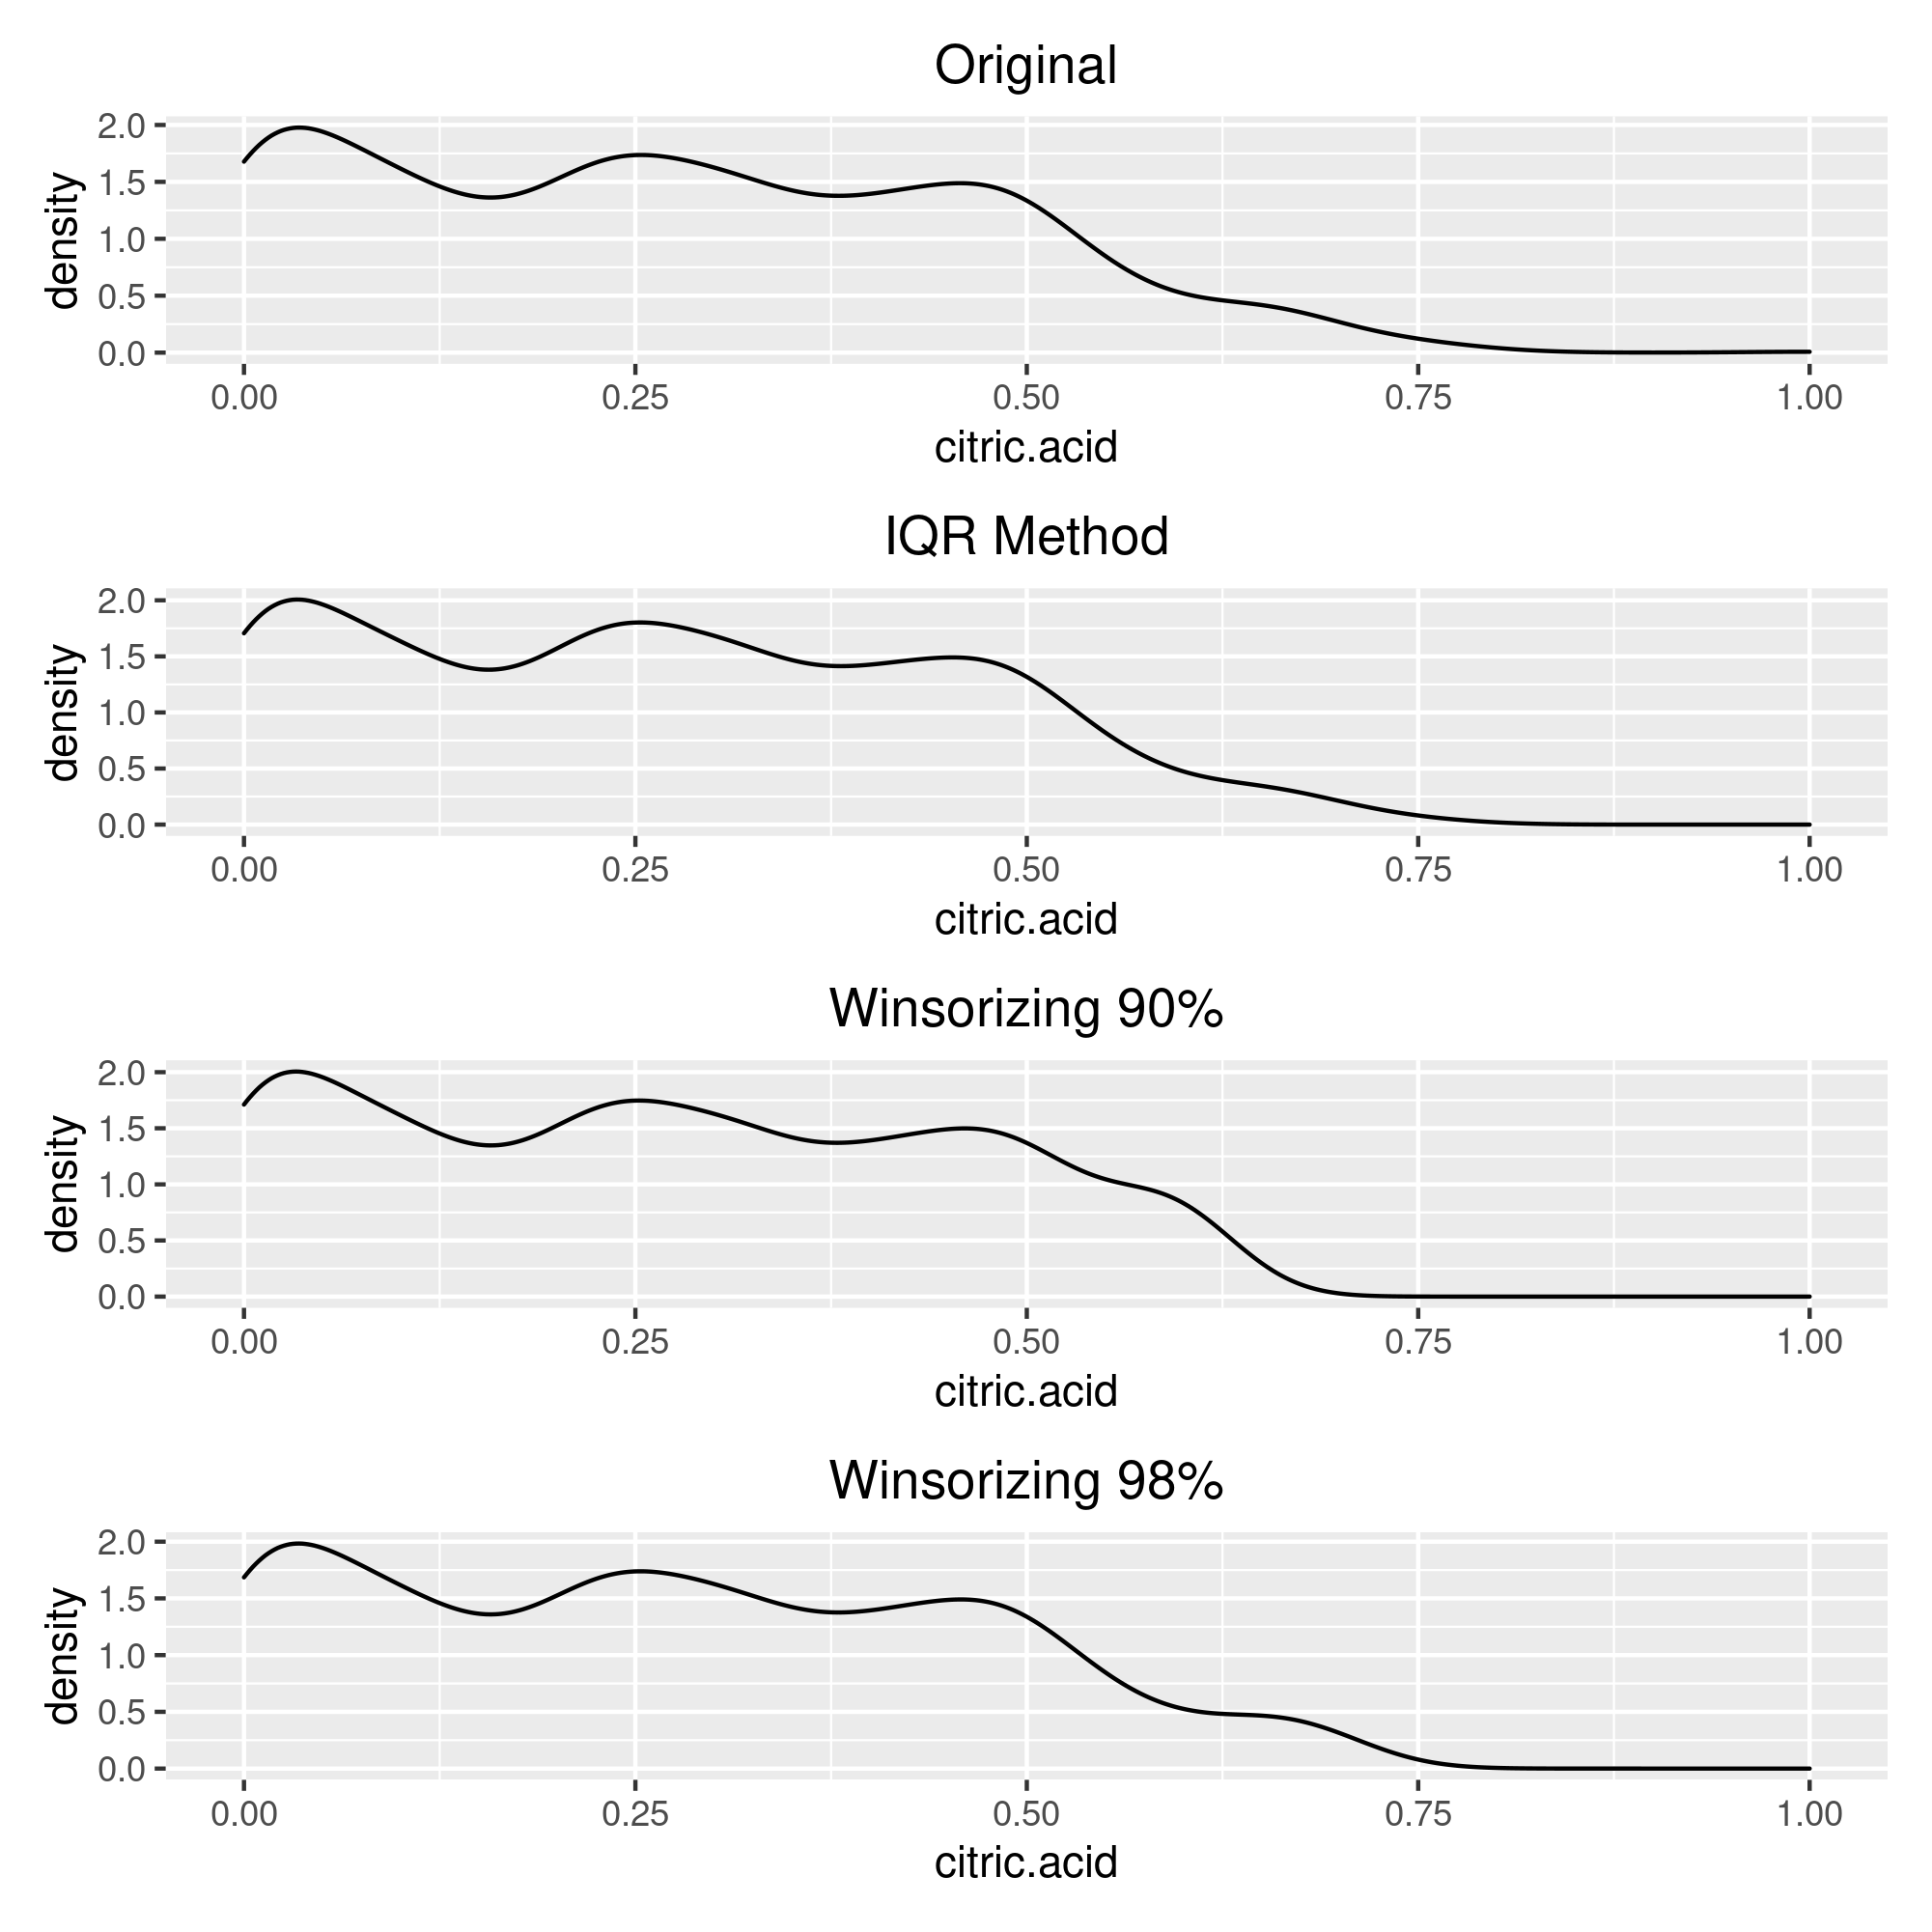
\includegraphics[width=0.45\textwidth]{images/outliers/citric.acid_distribution.png}
    }\qquad
    \subfloat[]{%
        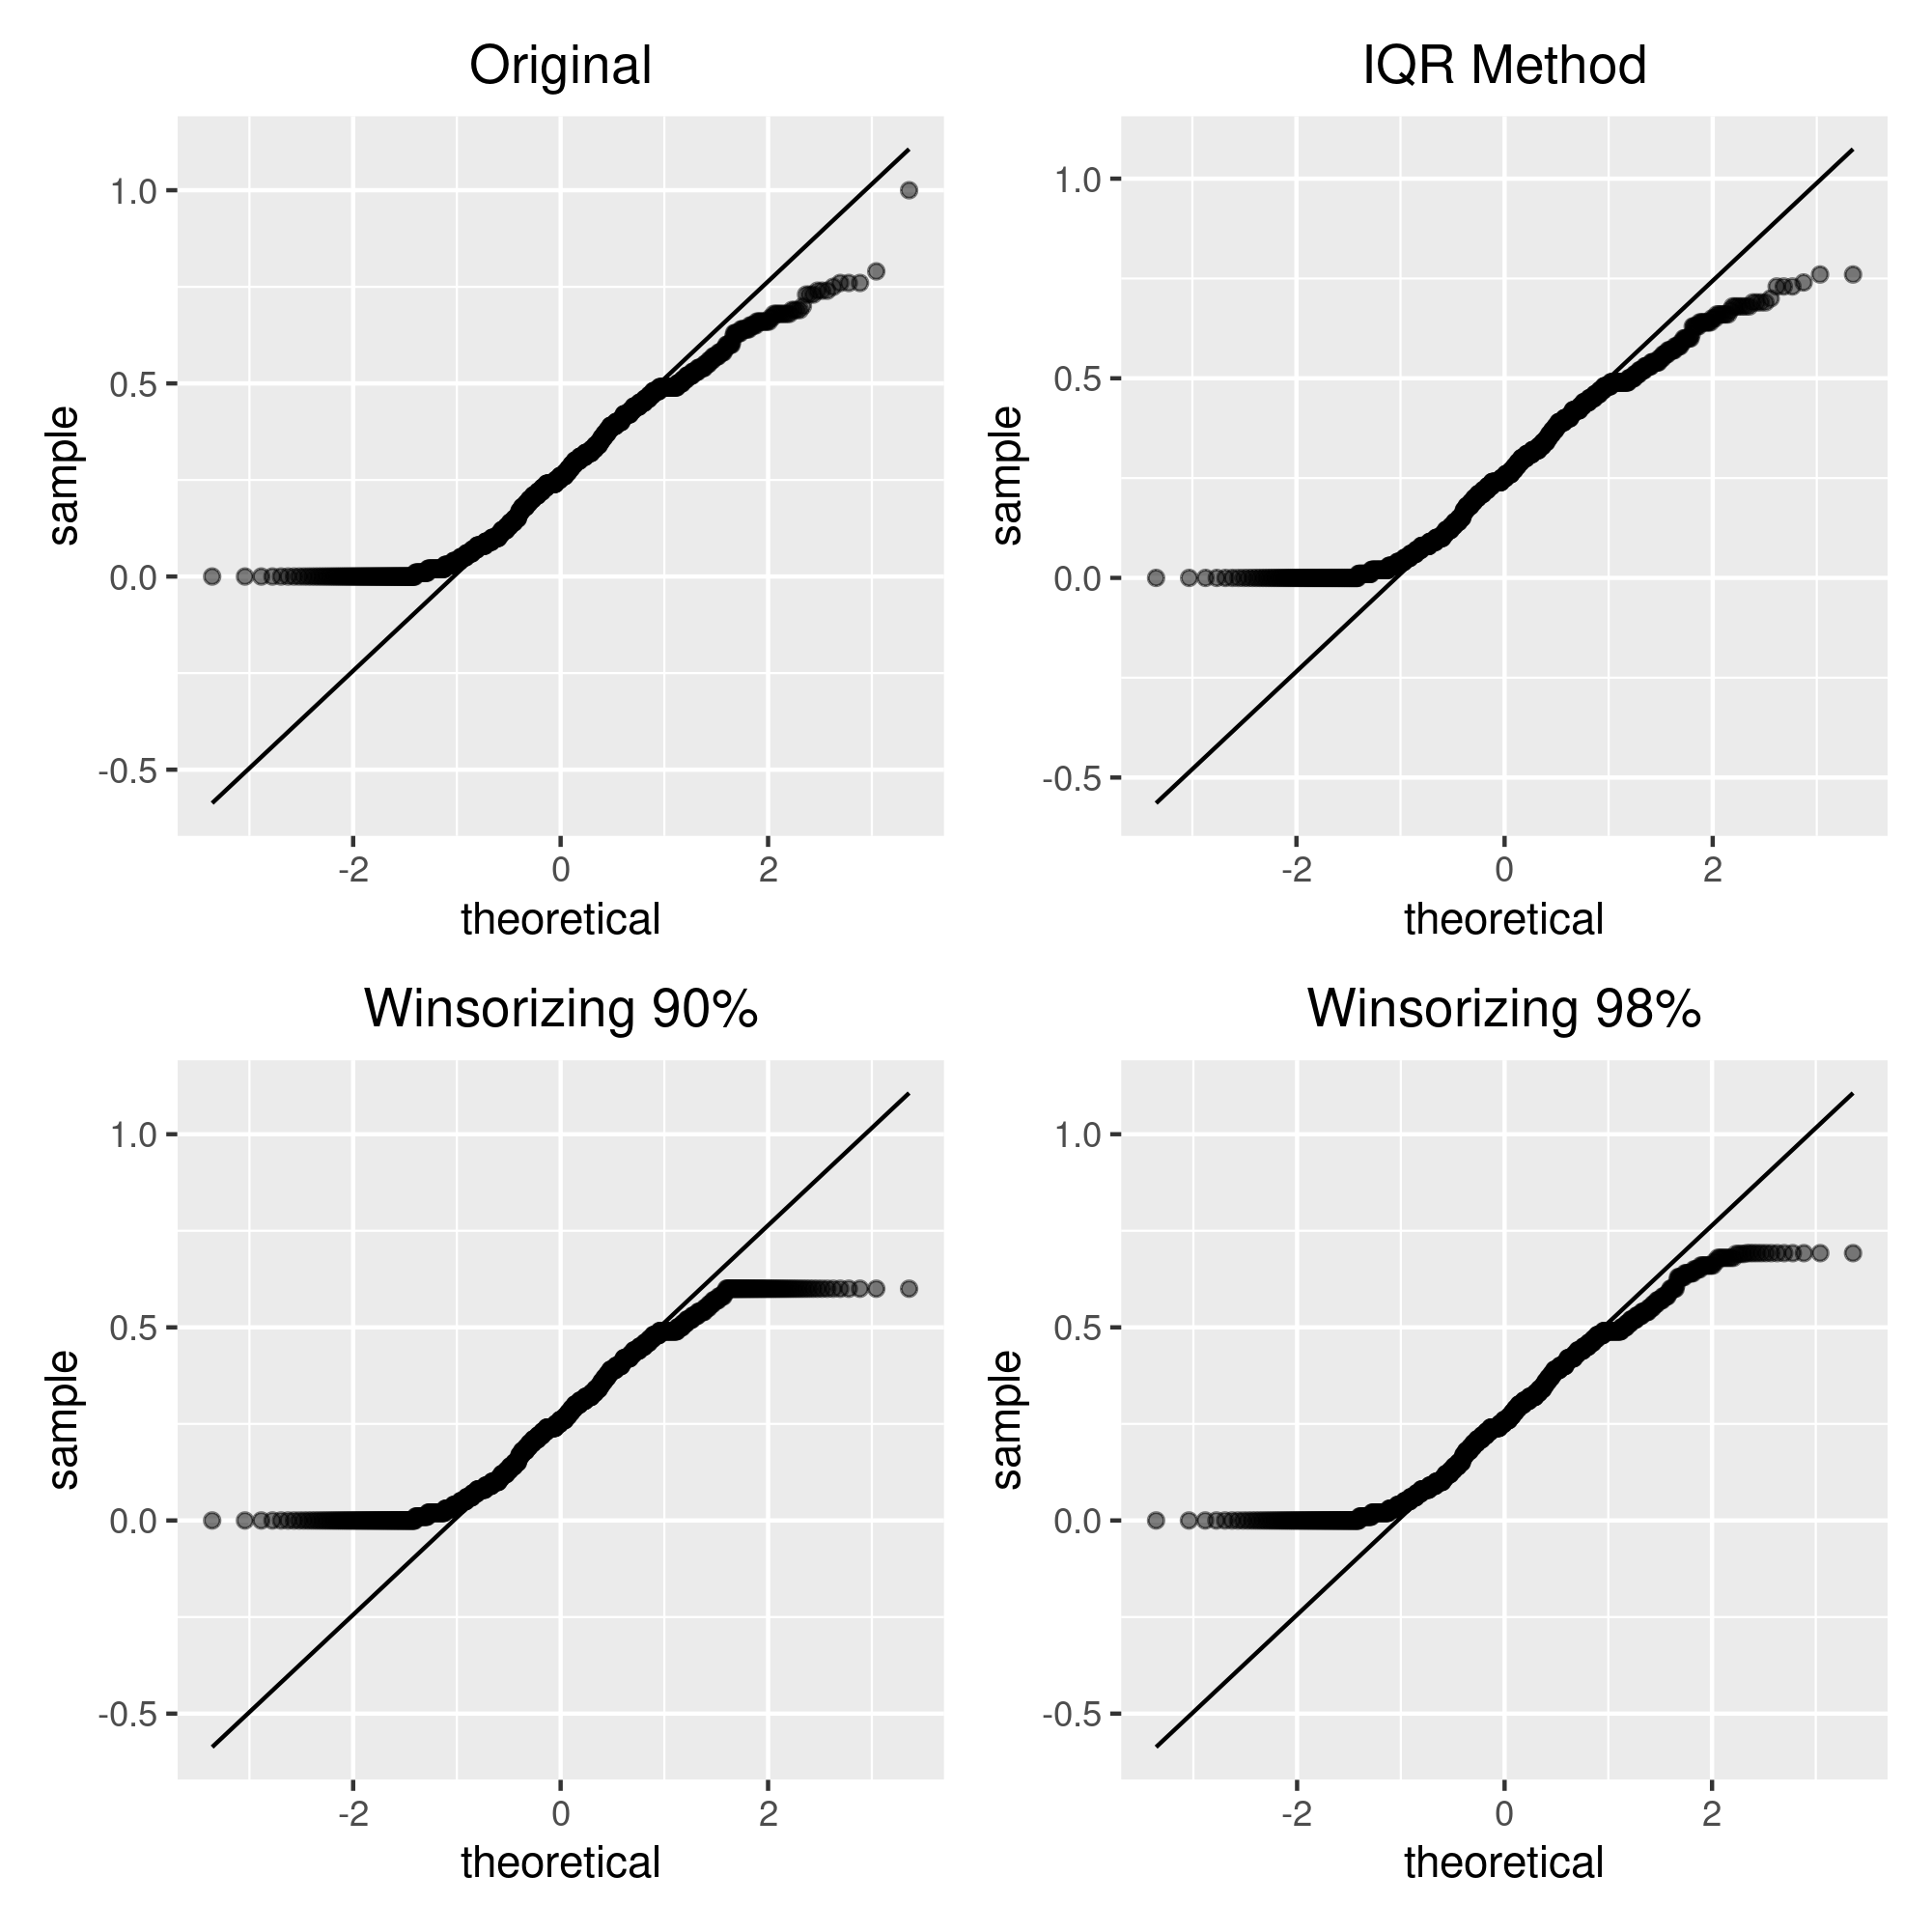
\includegraphics[width=0.45\textwidth]{images/outliers/citric.acid_qqplot.png}
    }

    \label{fig:outliers-citric.acid}
    \caption{Citric Acid}
\end{figure}

\begin{figure}[H]
    \centering

    \subfloat[]{%
        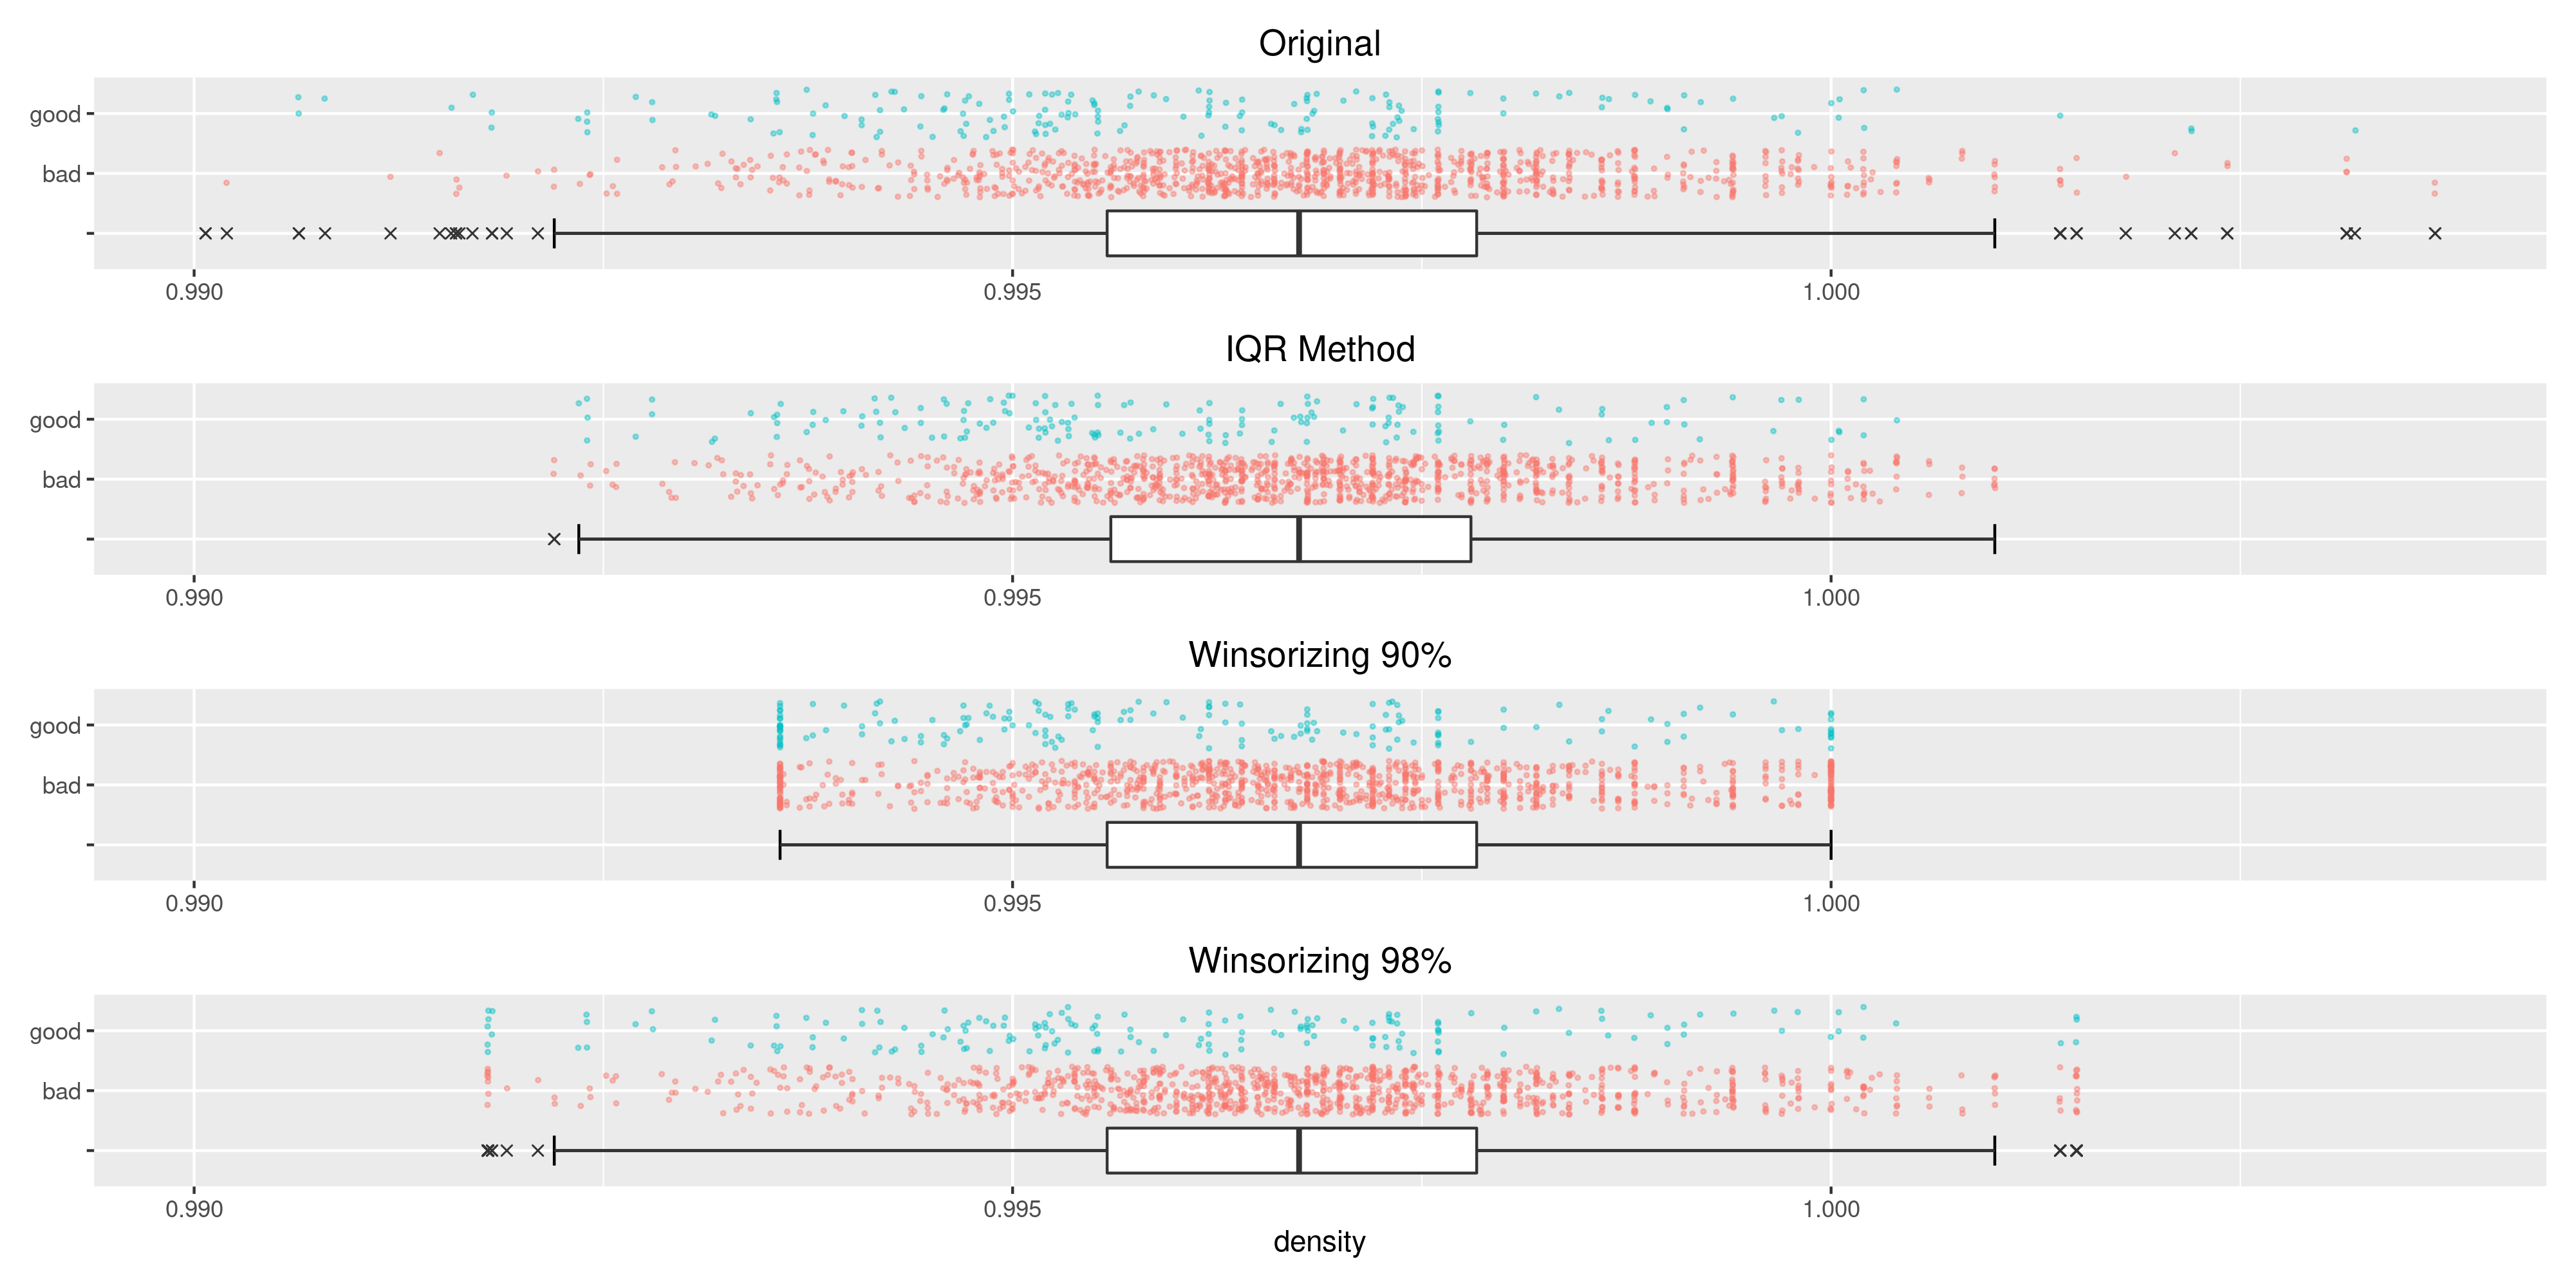
\includegraphics[width=0.99\textwidth]{images/outliers/density_boxplot.png}
    }

    \subfloat[]{%
        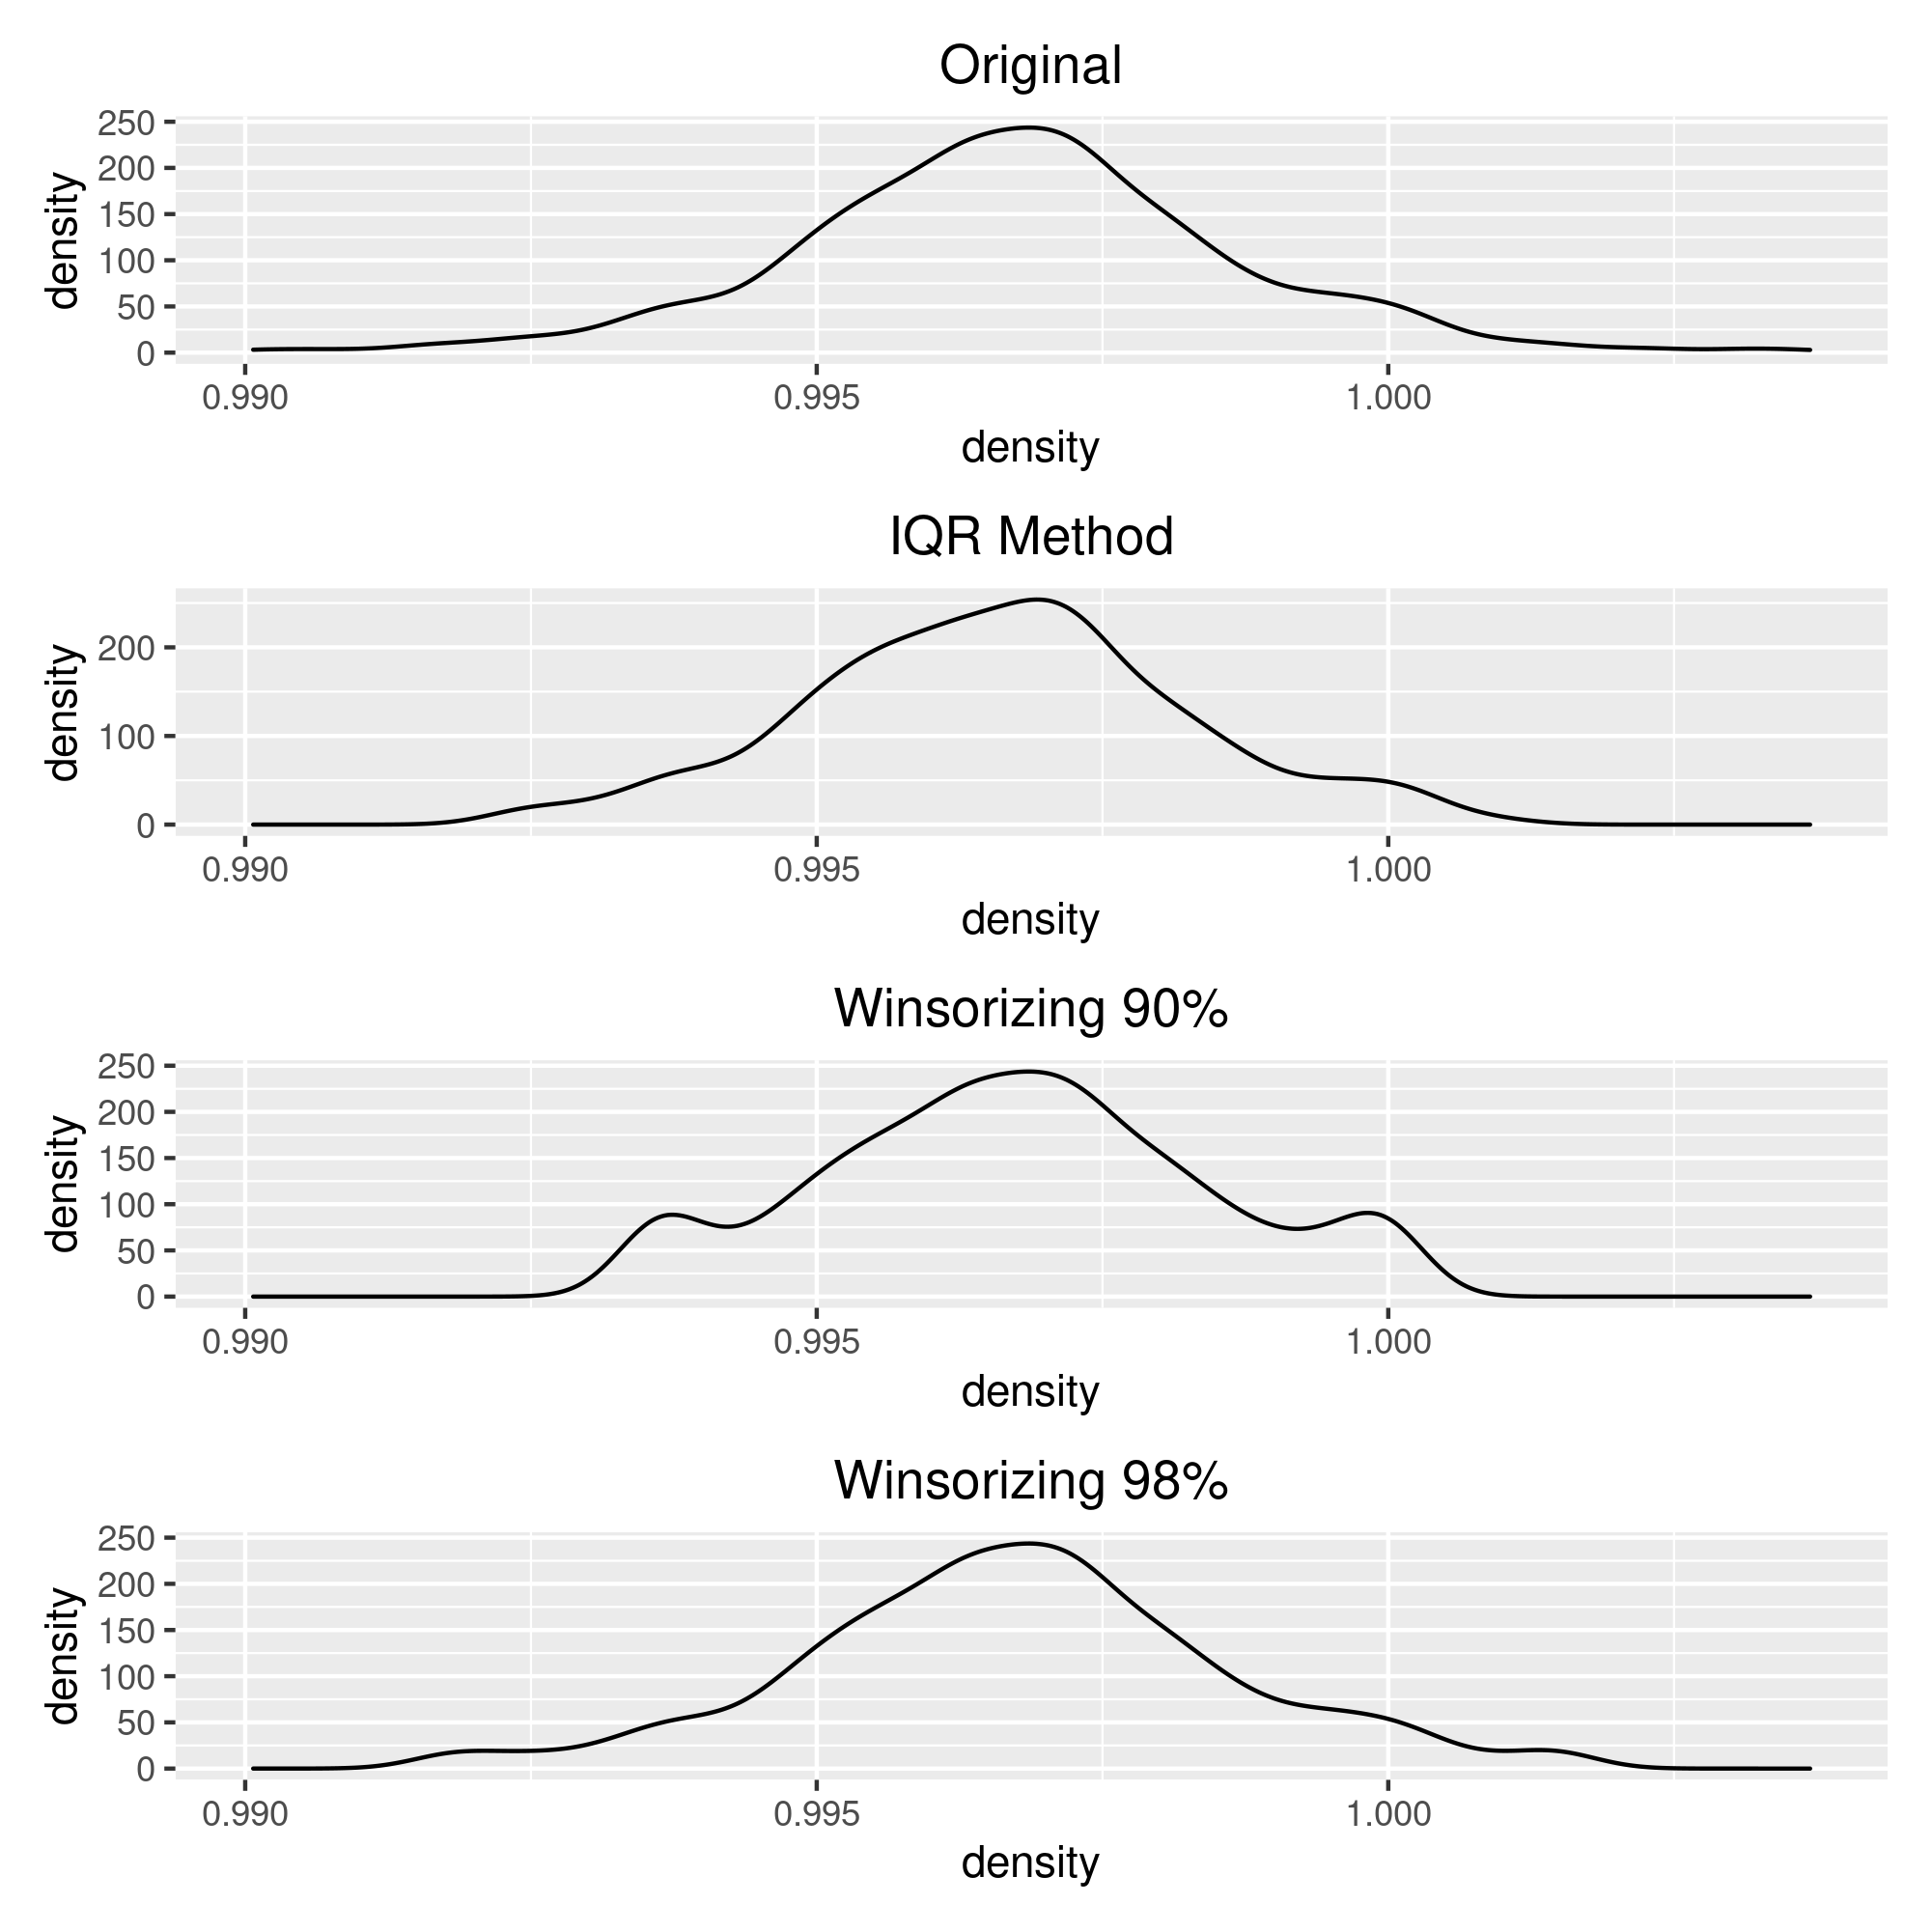
\includegraphics[width=0.45\textwidth]{images/outliers/density_distribution.png}
    }\qquad
    \subfloat[]{%
        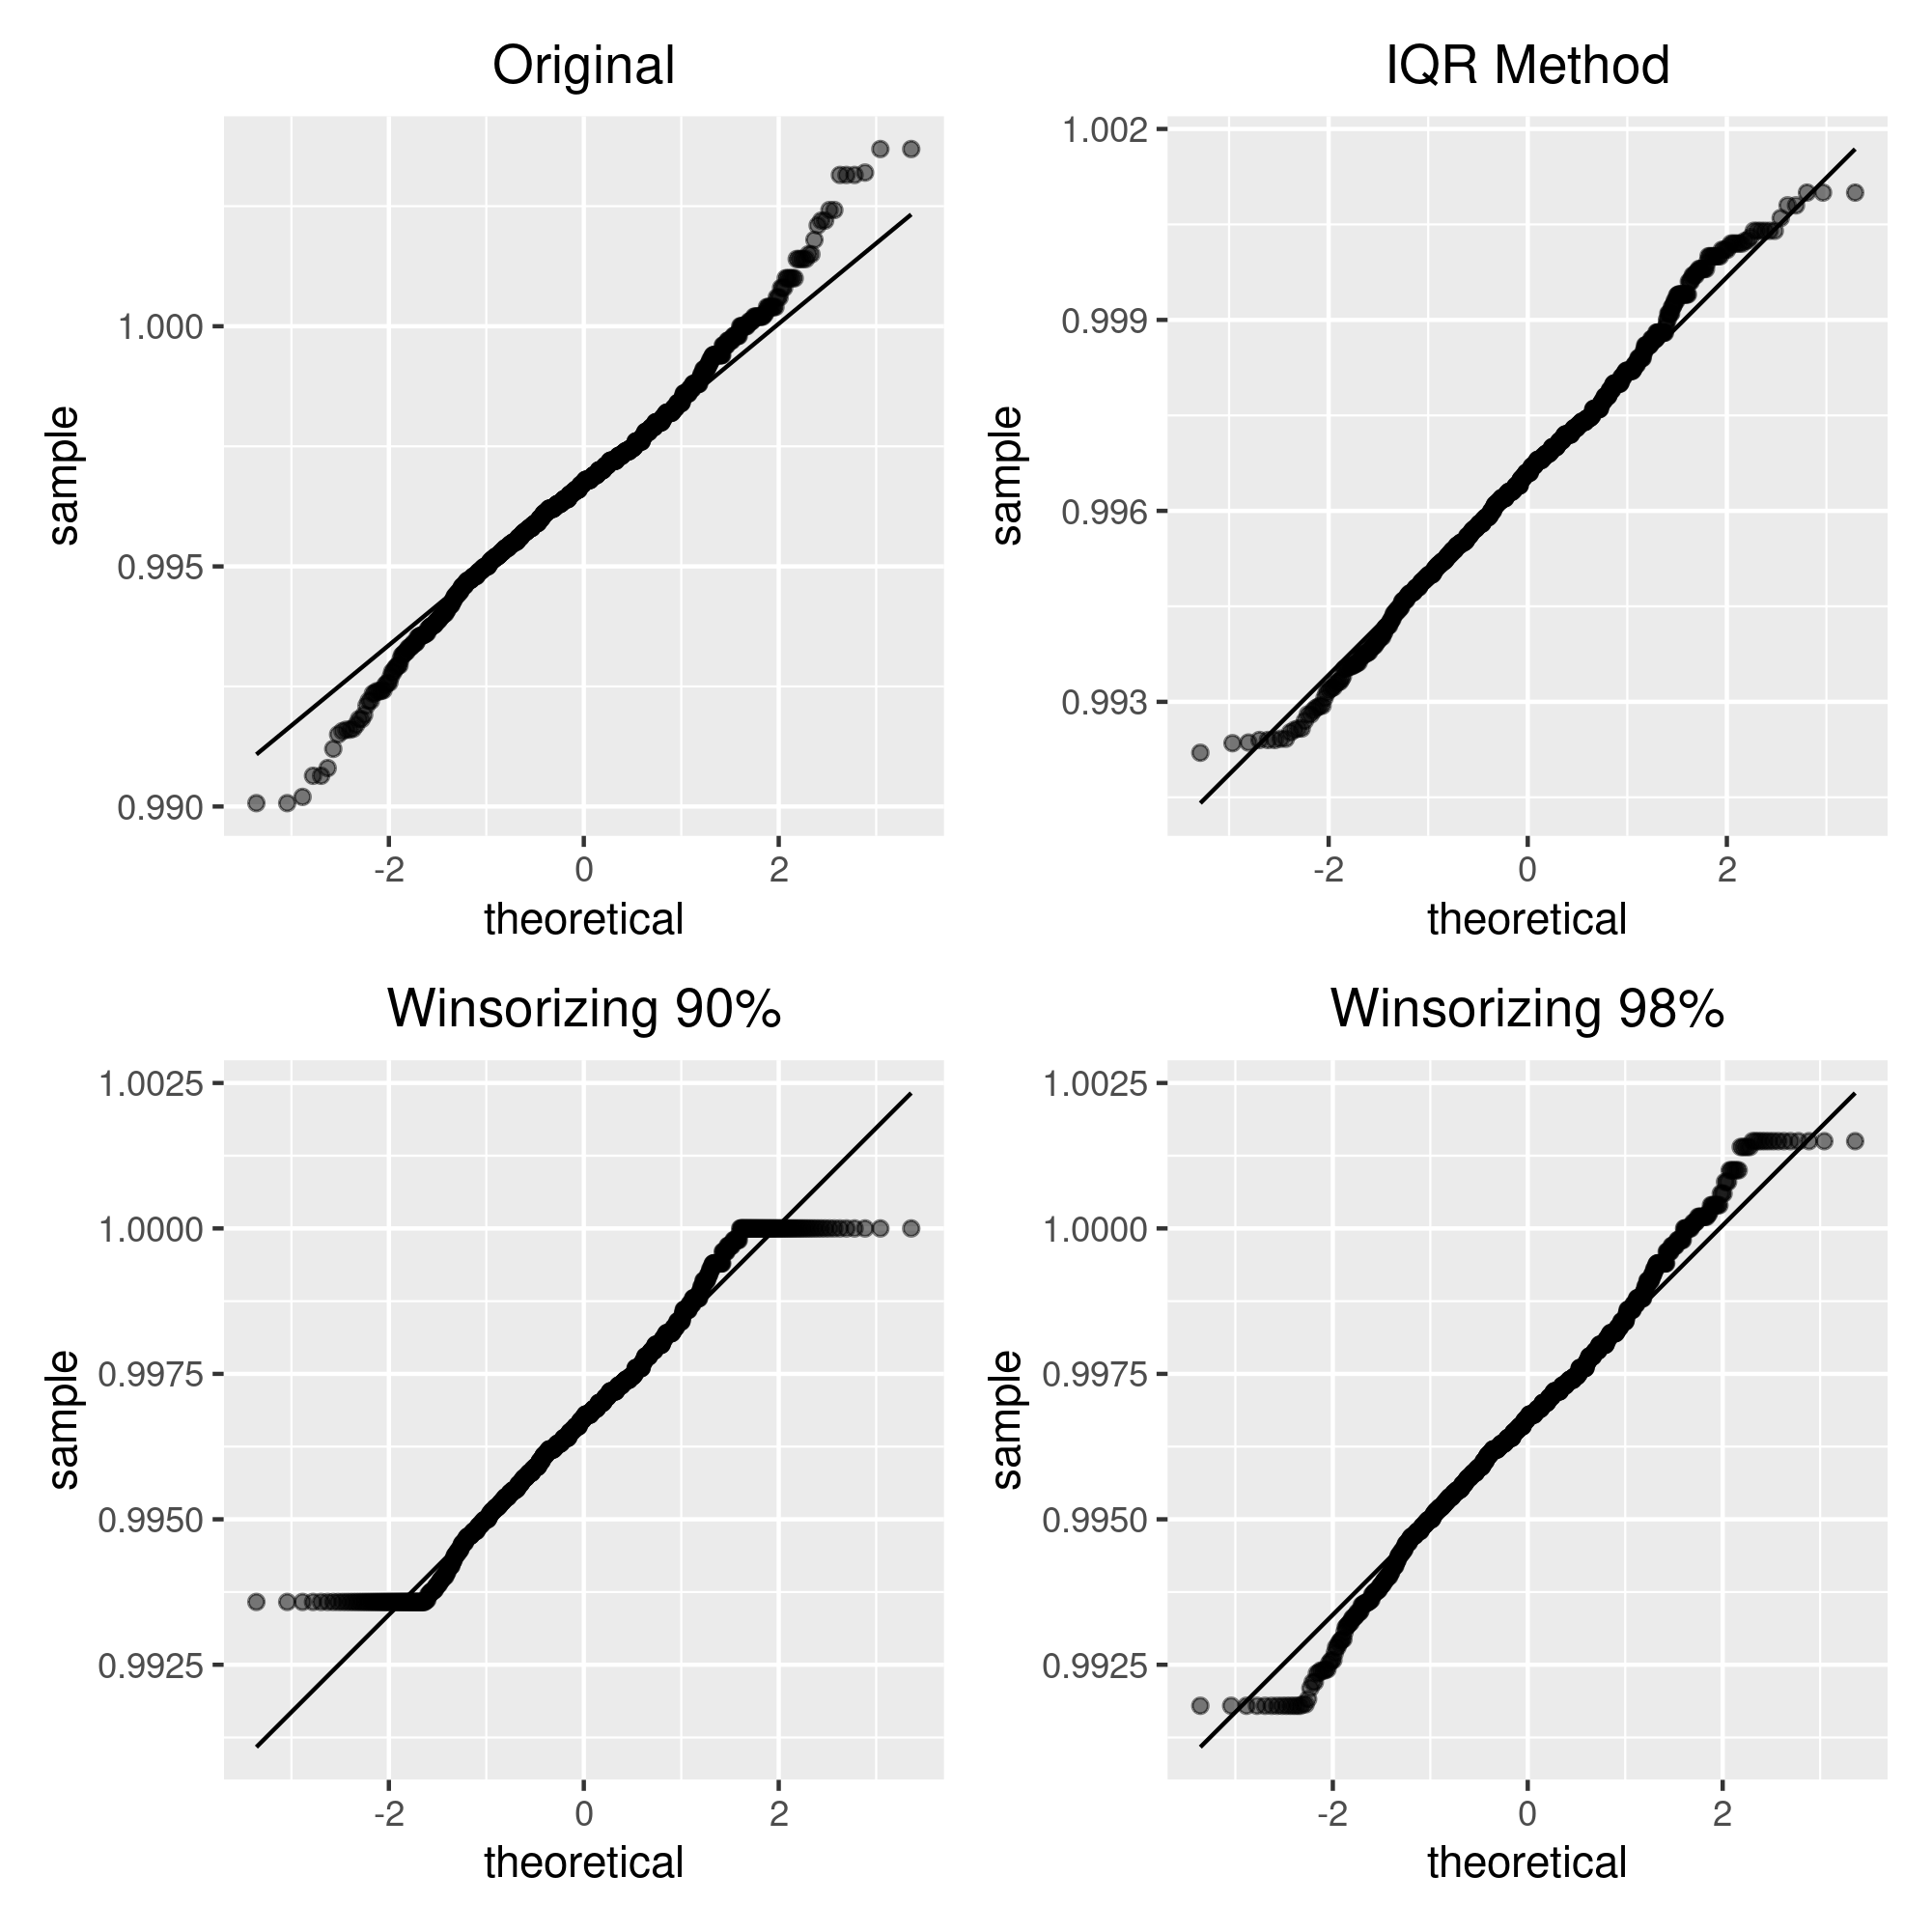
\includegraphics[width=0.45\textwidth]{images/outliers/density_qqplot.png}
    }

    \label{fig:outliers-density}
    \caption{Density}
\end{figure}

\begin{figure}[H]
    \centering

    \subfloat[]{%
        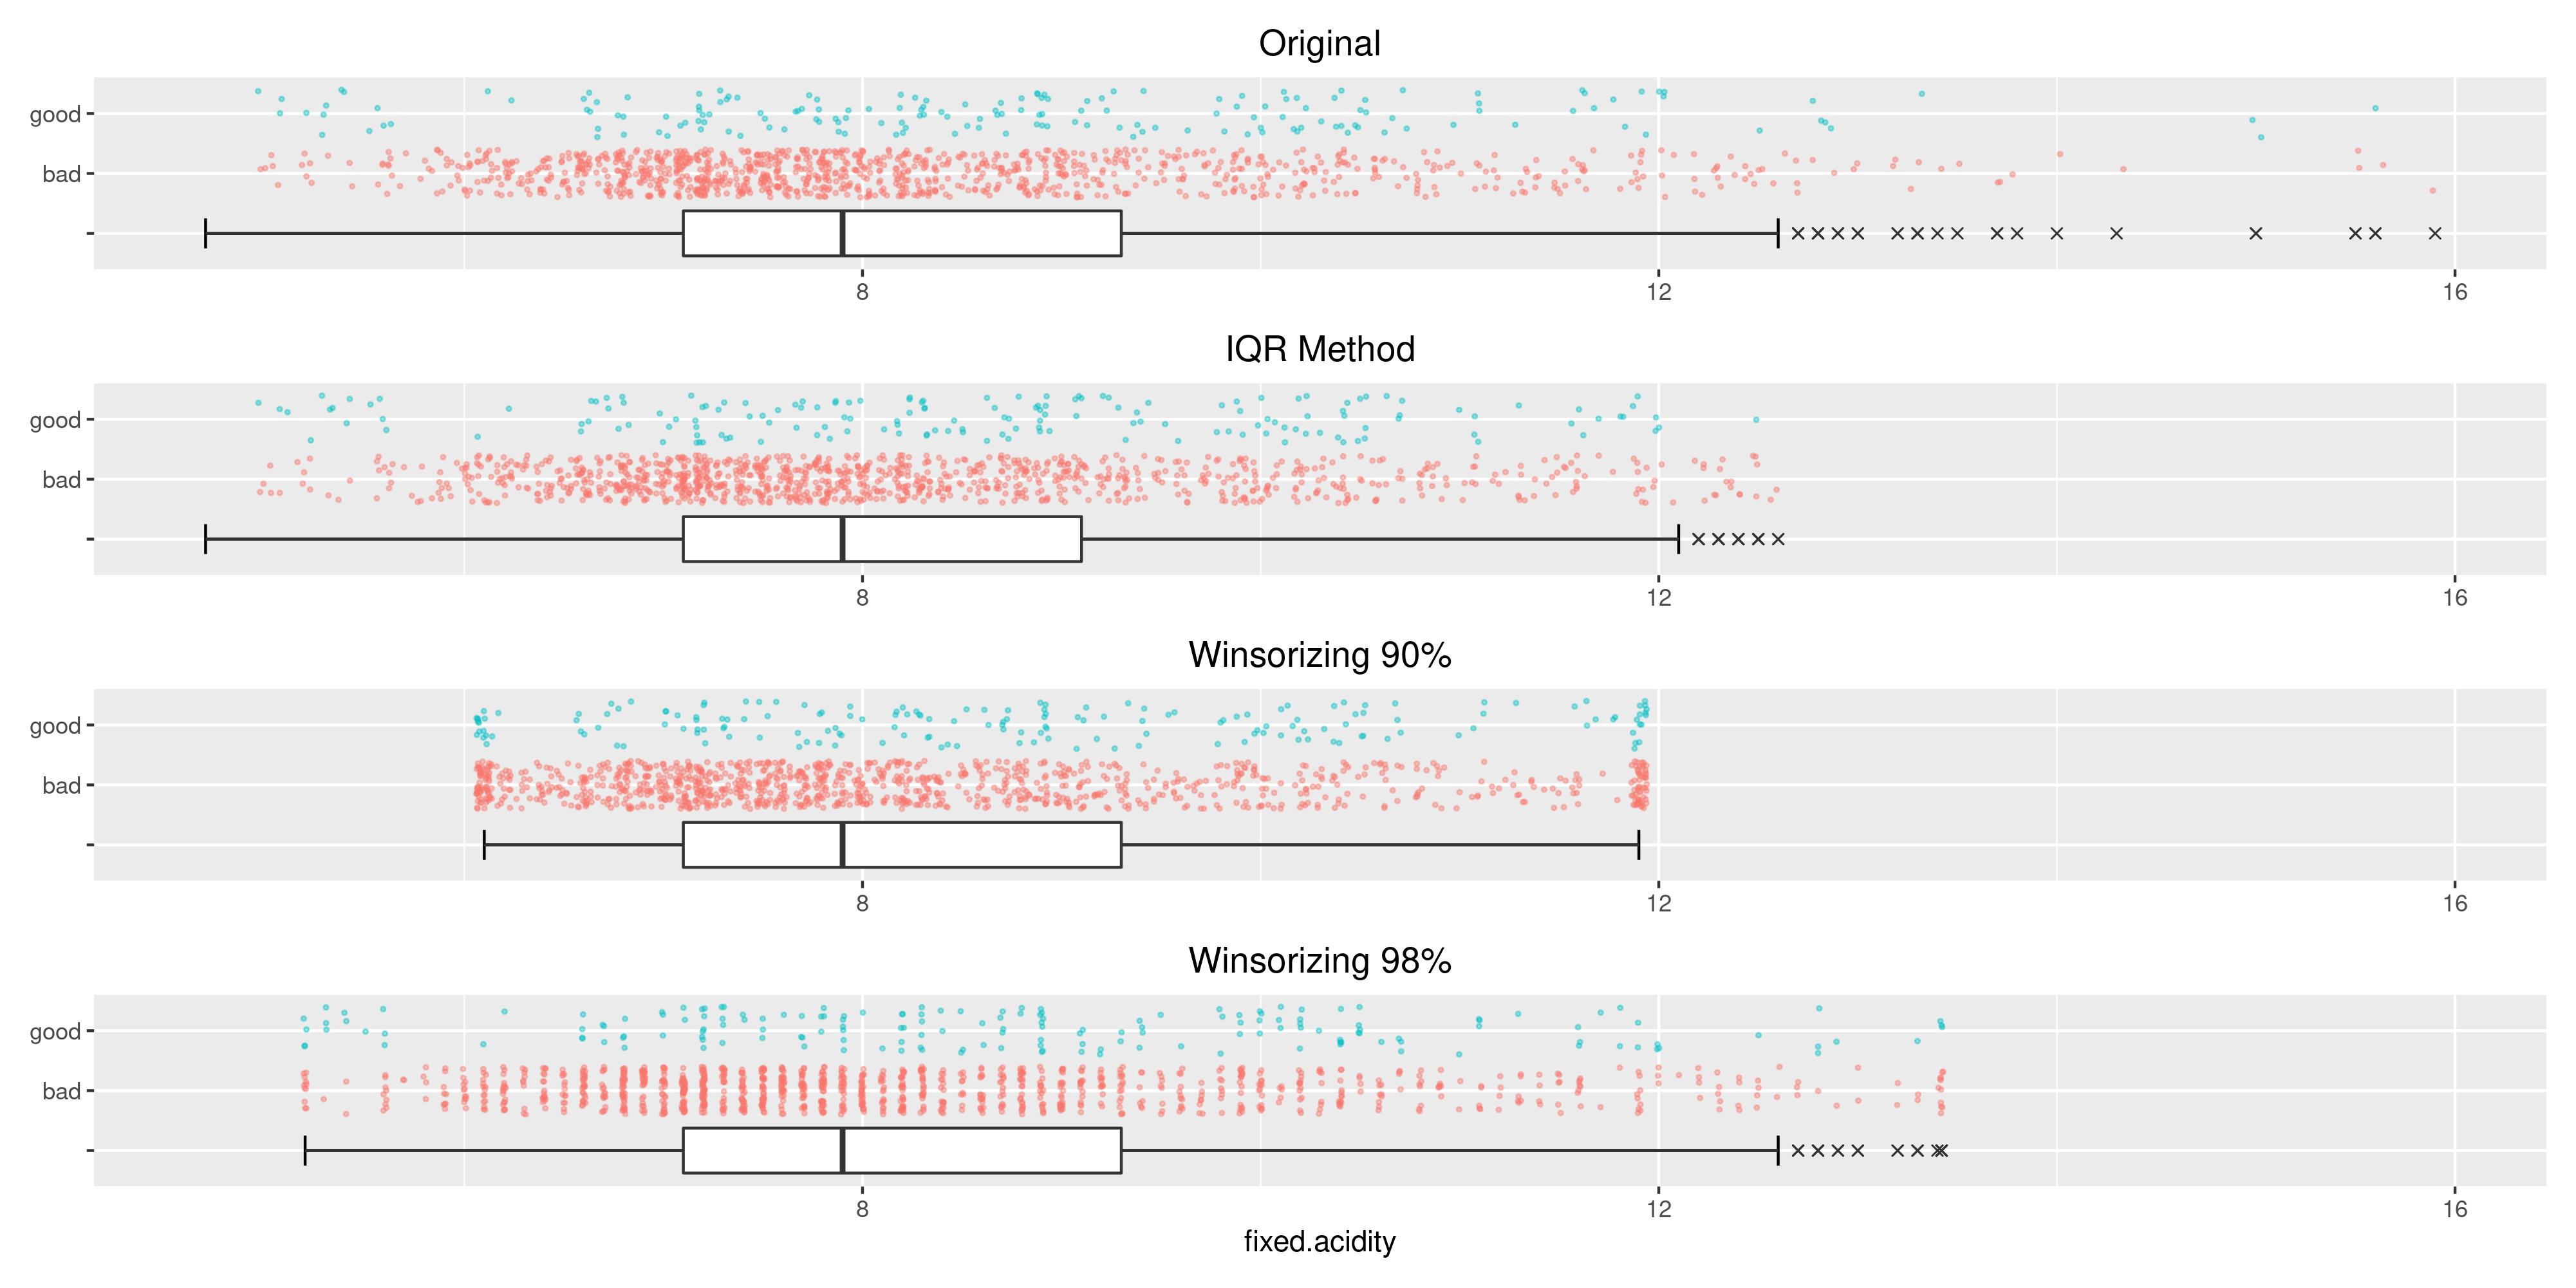
\includegraphics[width=0.99\textwidth]{images/outliers/fixed.acidity_boxplot.png}
    }

    \subfloat[]{%
        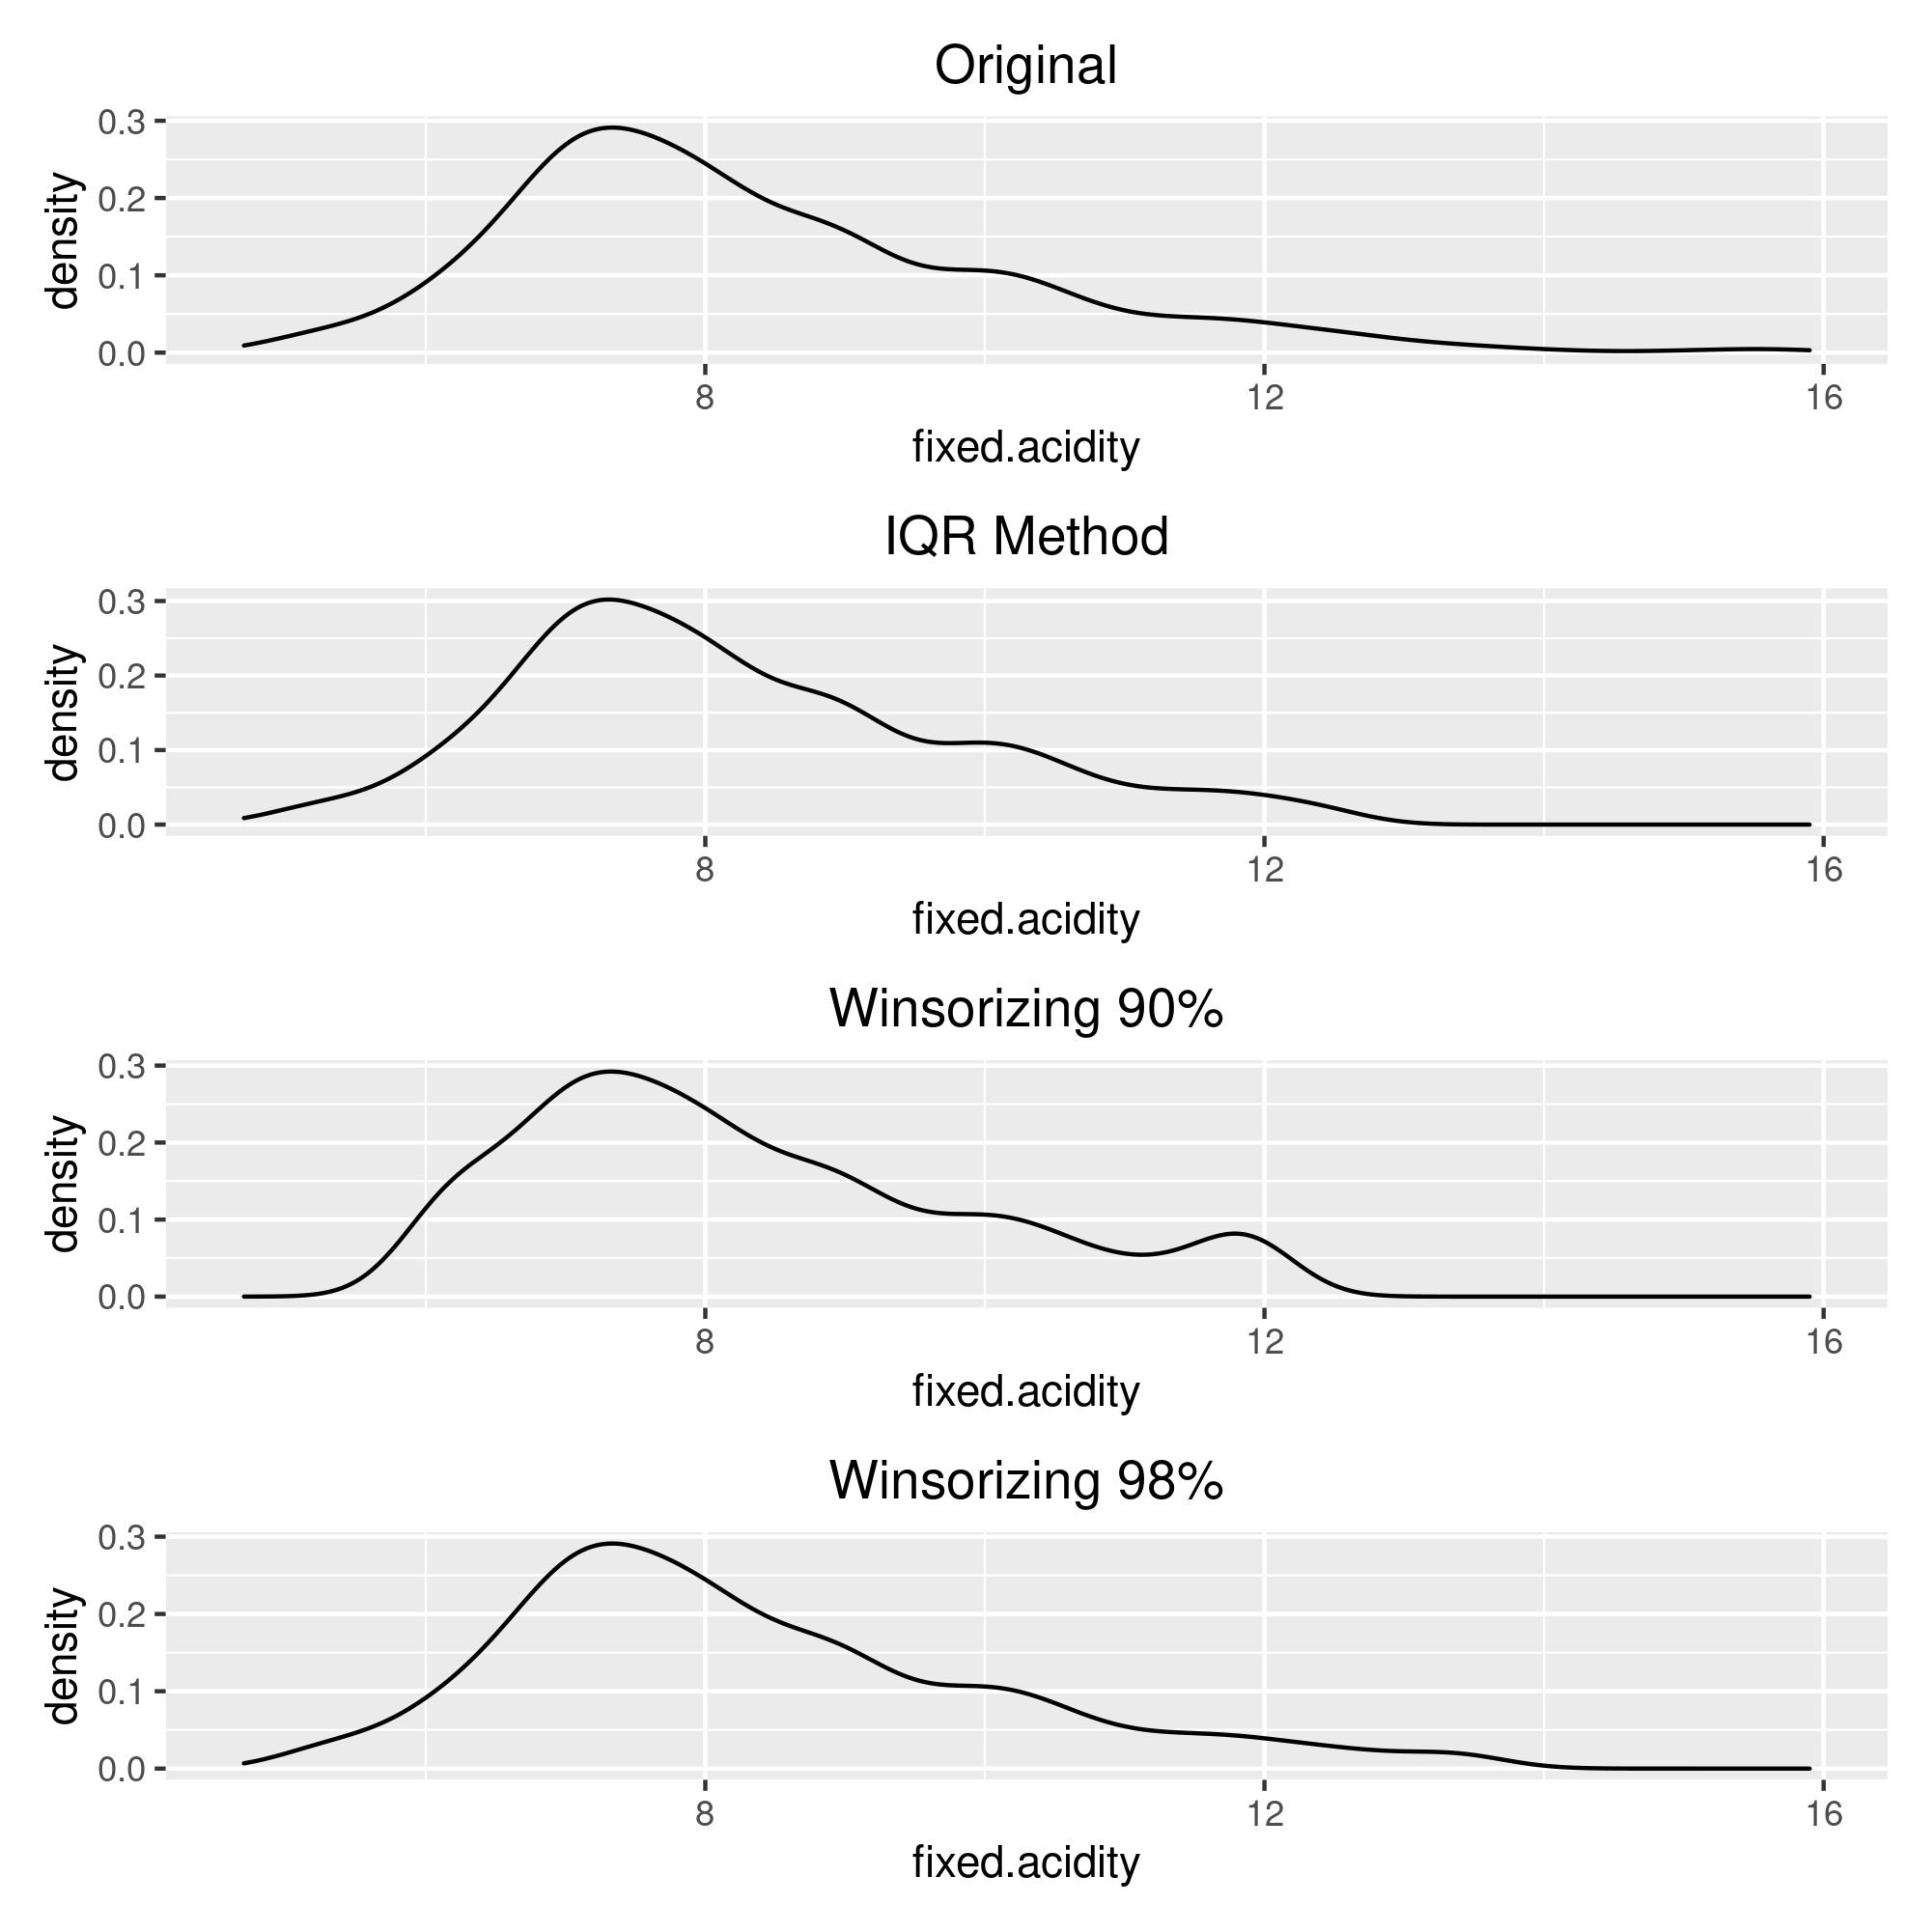
\includegraphics[width=0.45\textwidth]{images/outliers/fixed.acidity_distribution.png}
    }\qquad
    \subfloat[]{%
        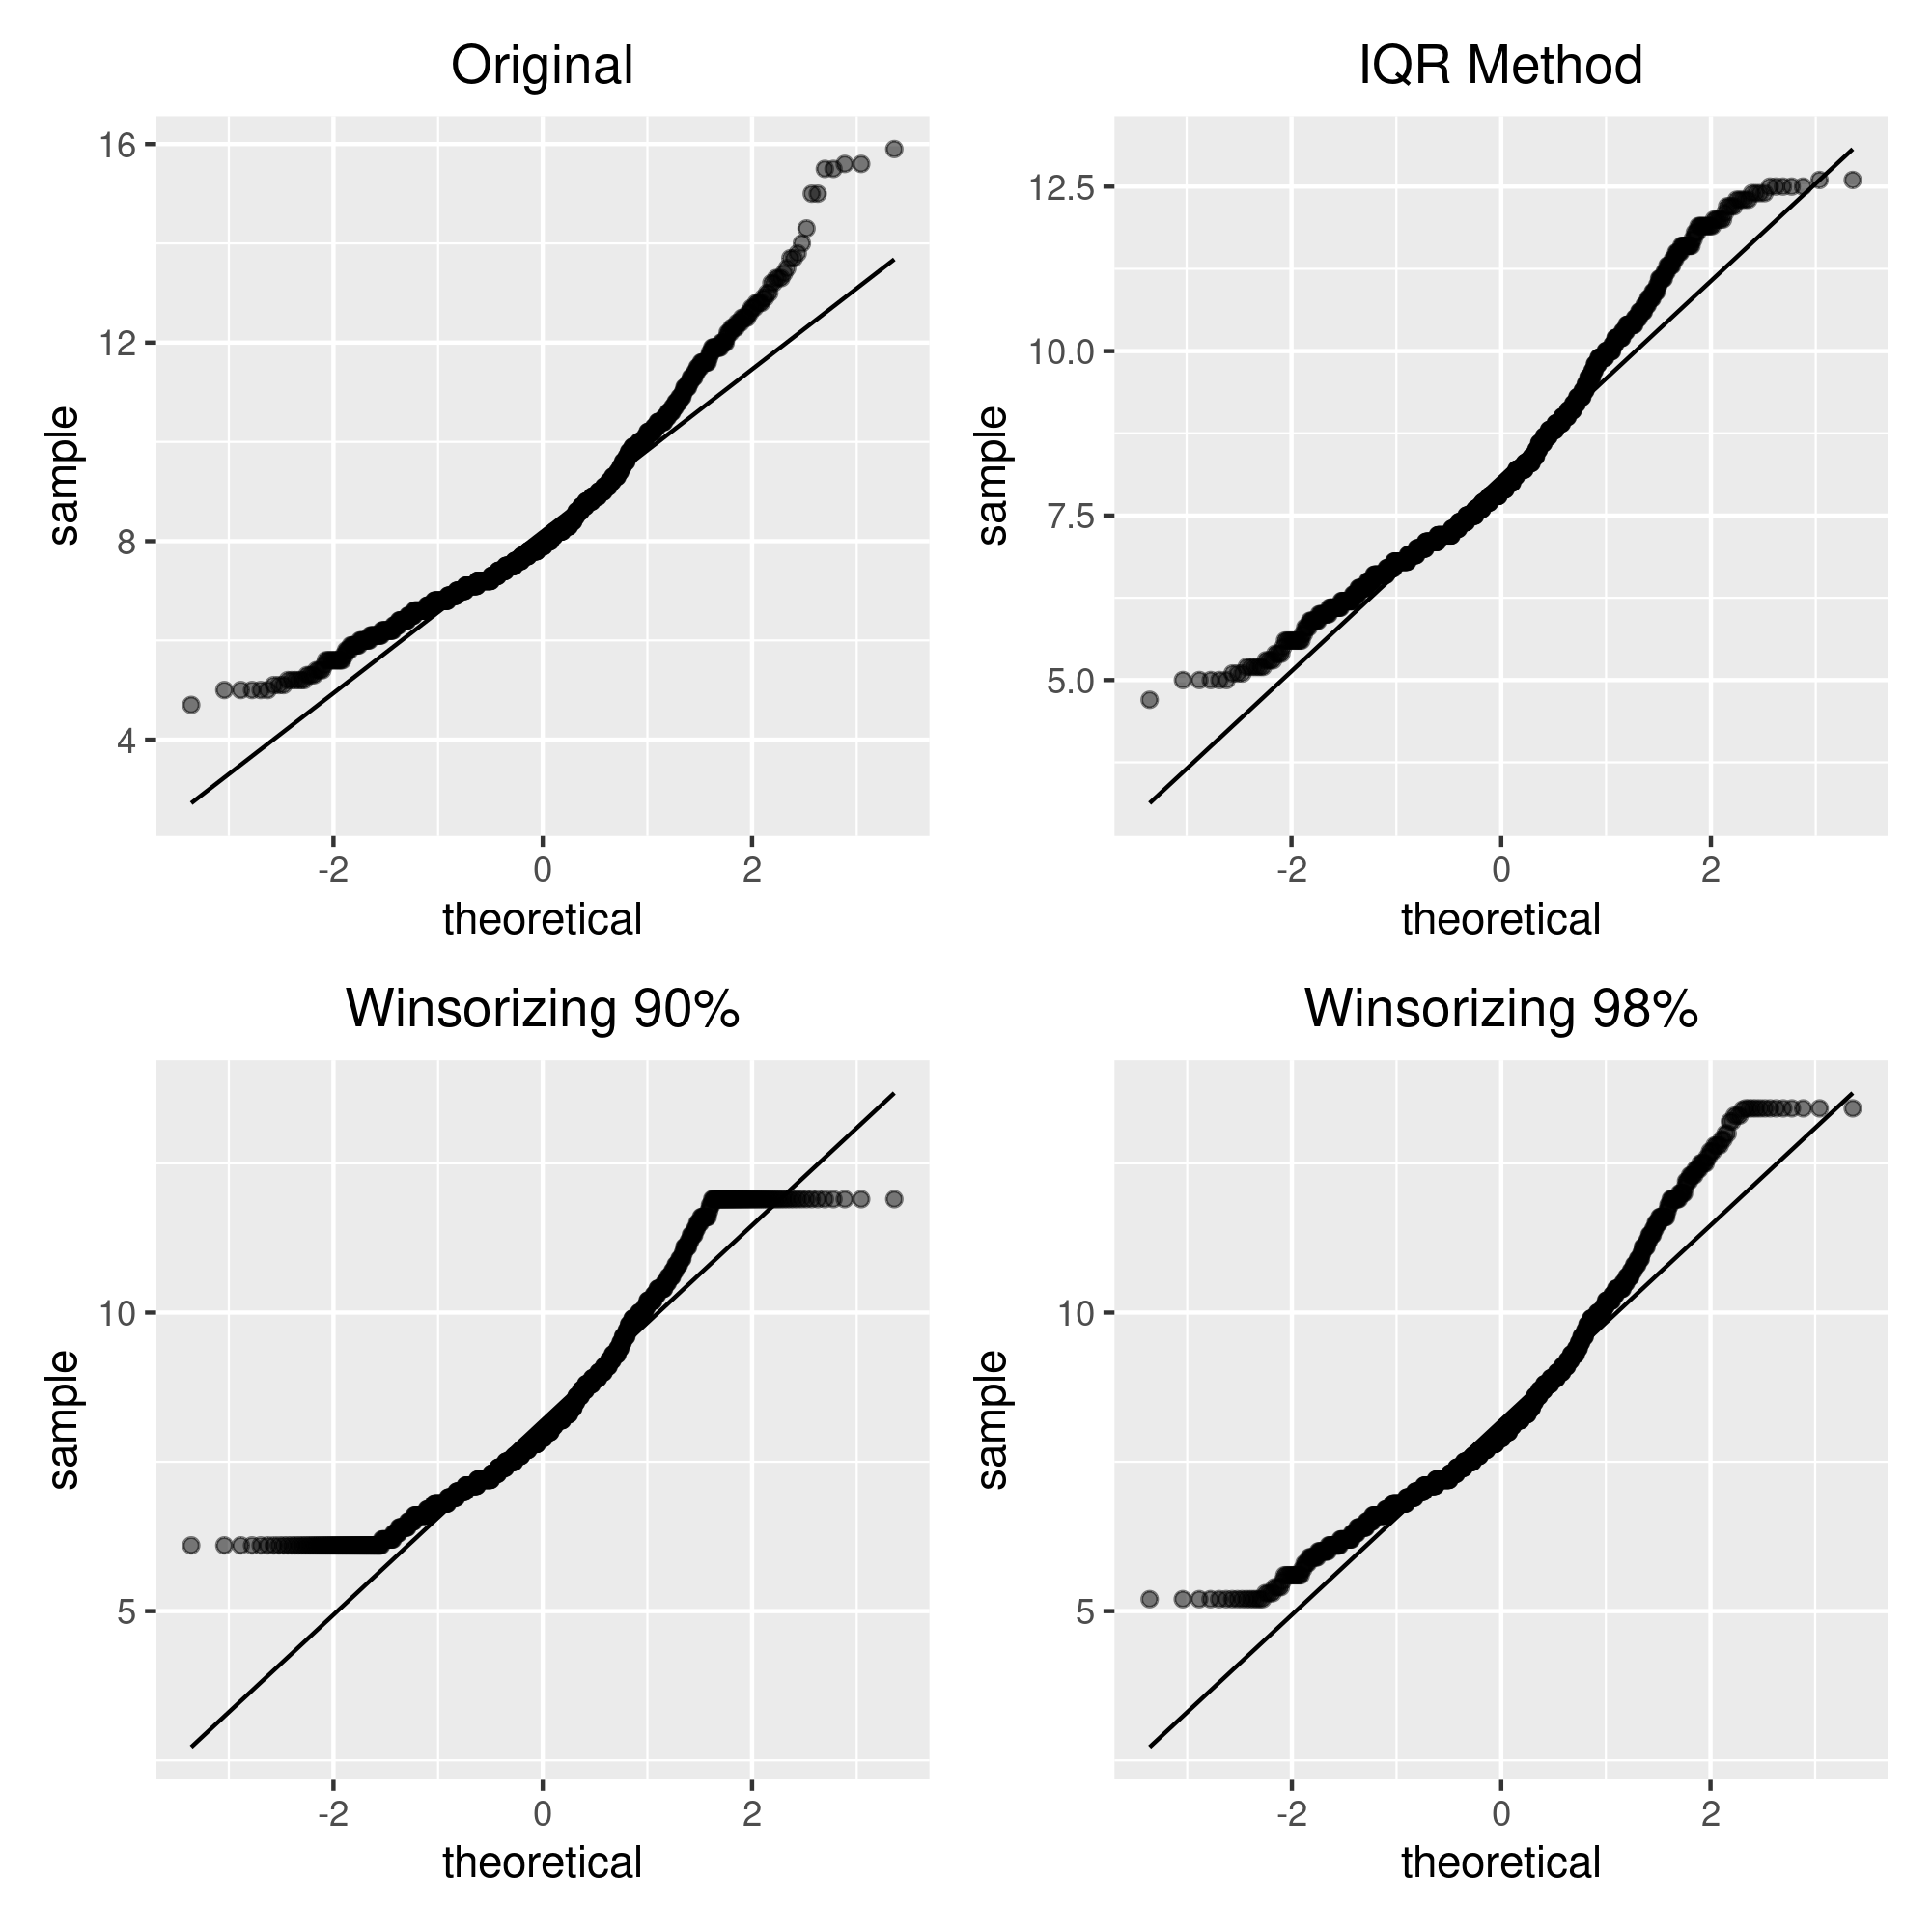
\includegraphics[width=0.45\textwidth]{images/outliers/fixed.acidity_qqplot.png}
    }

    \label{fig:outliers-fixed.acidity}
    \caption{Fixed Acidity}
\end{figure}

\begin{figure}[H]
    \centering

    \subfloat[]{%
        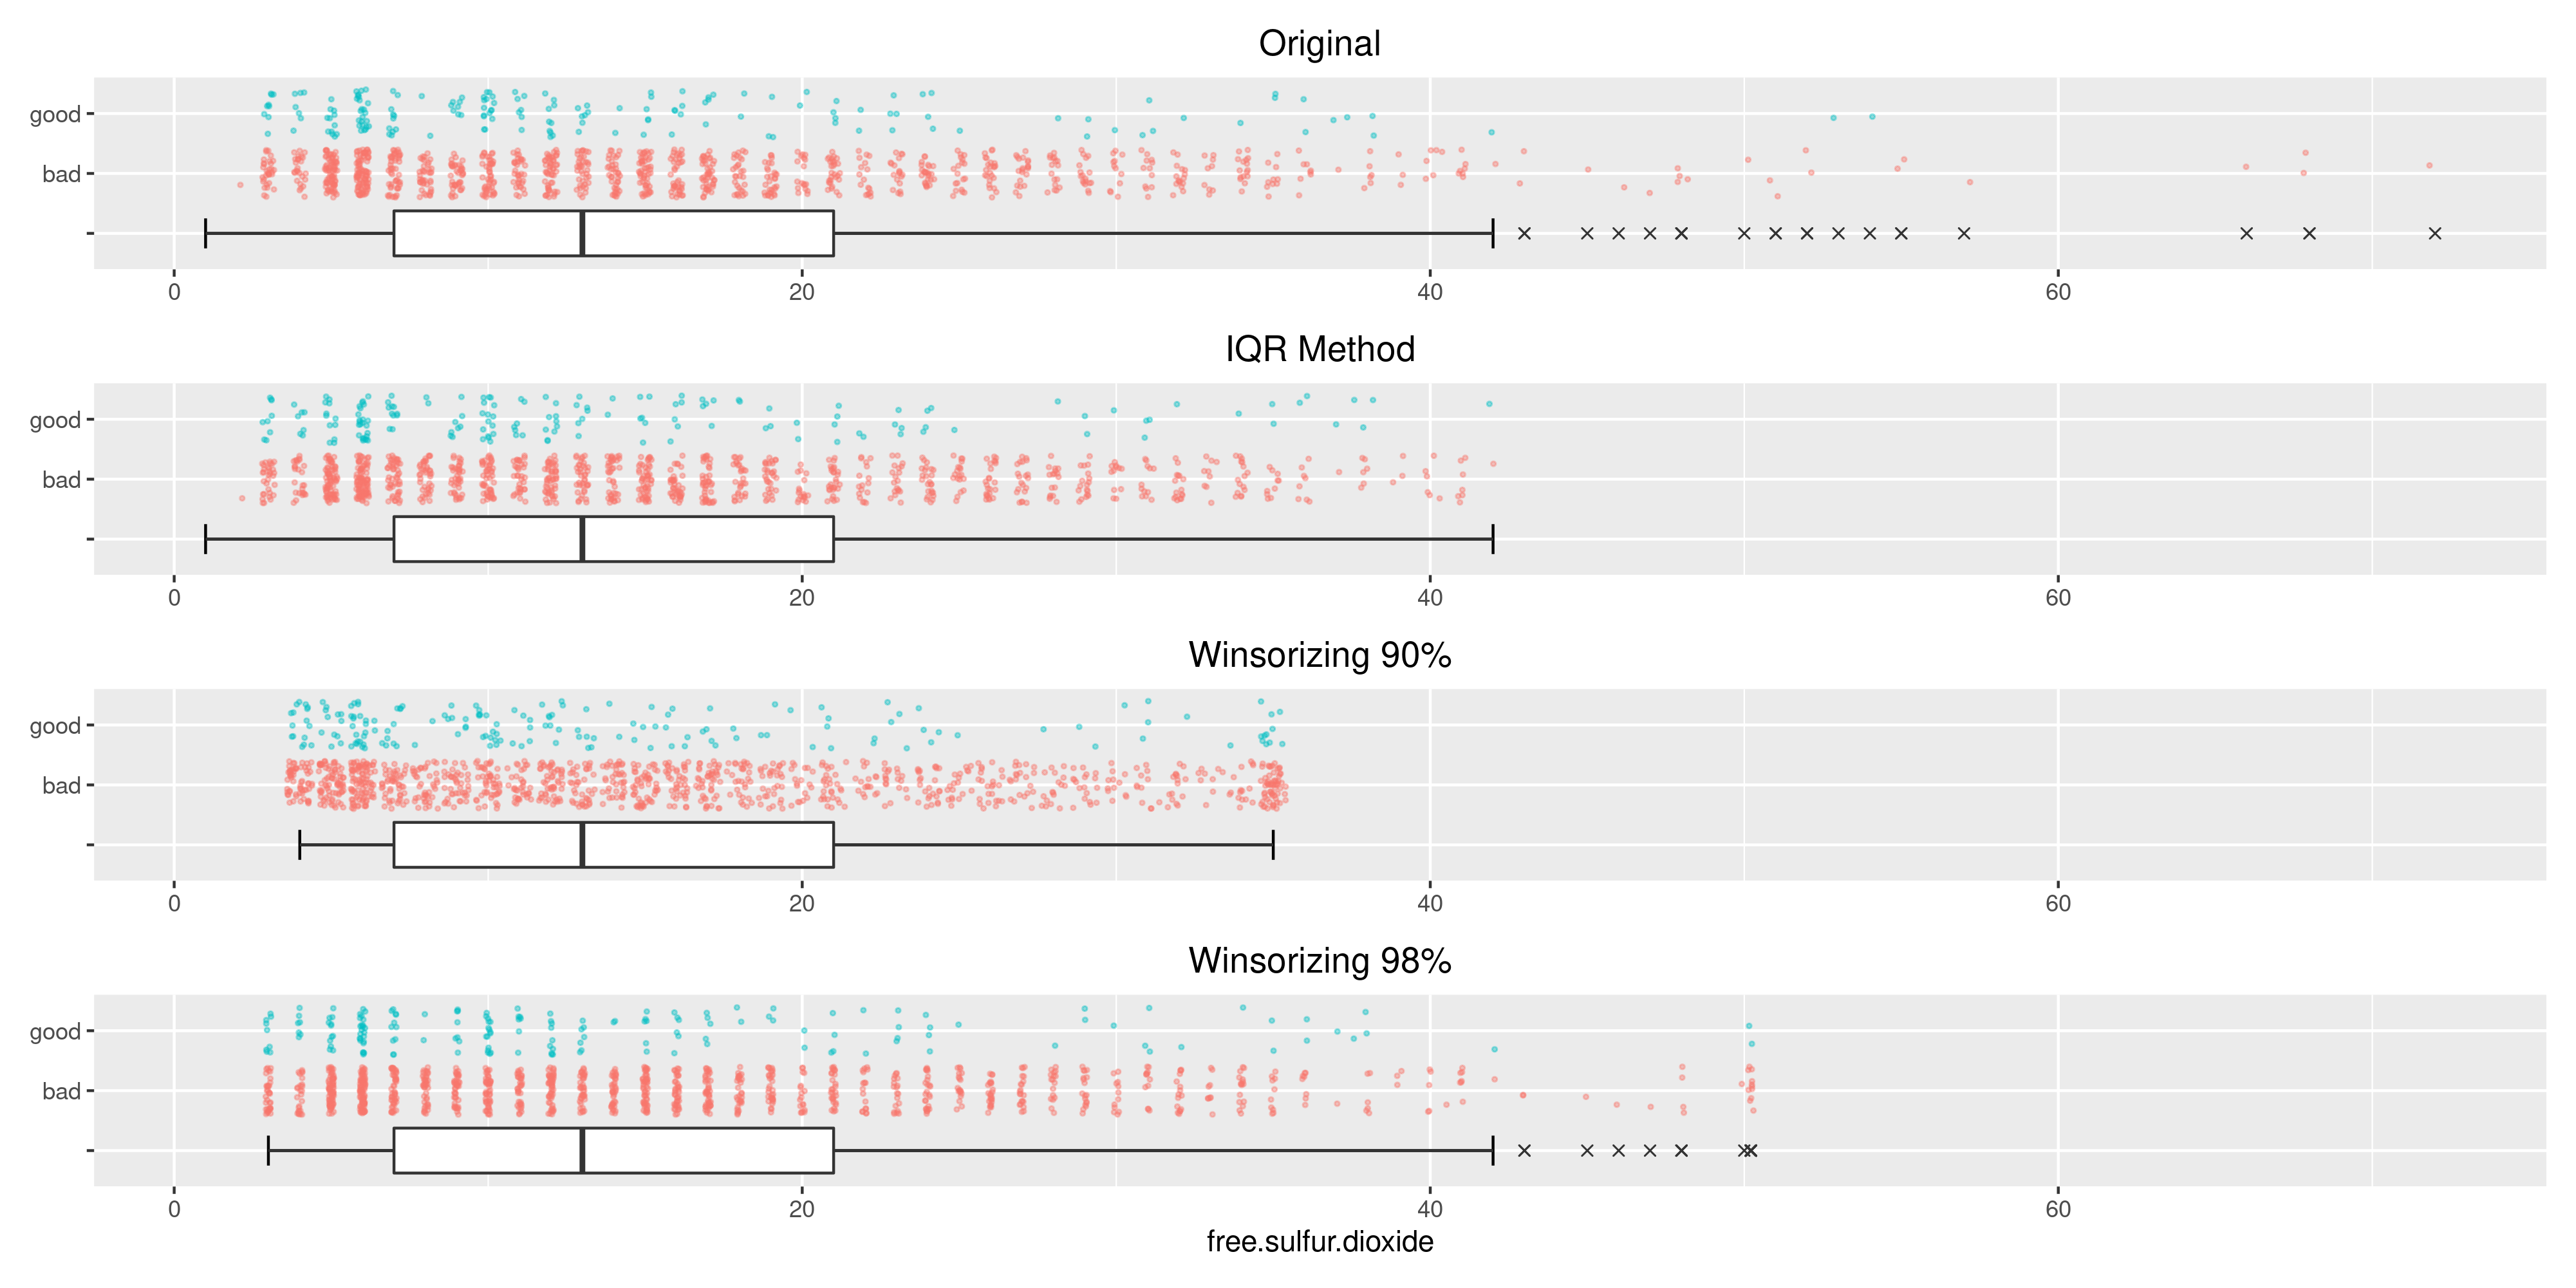
\includegraphics[width=0.99\textwidth]{images/outliers/free.sulfur.dioxide_boxplot.png}
    }

    \subfloat[]{%
        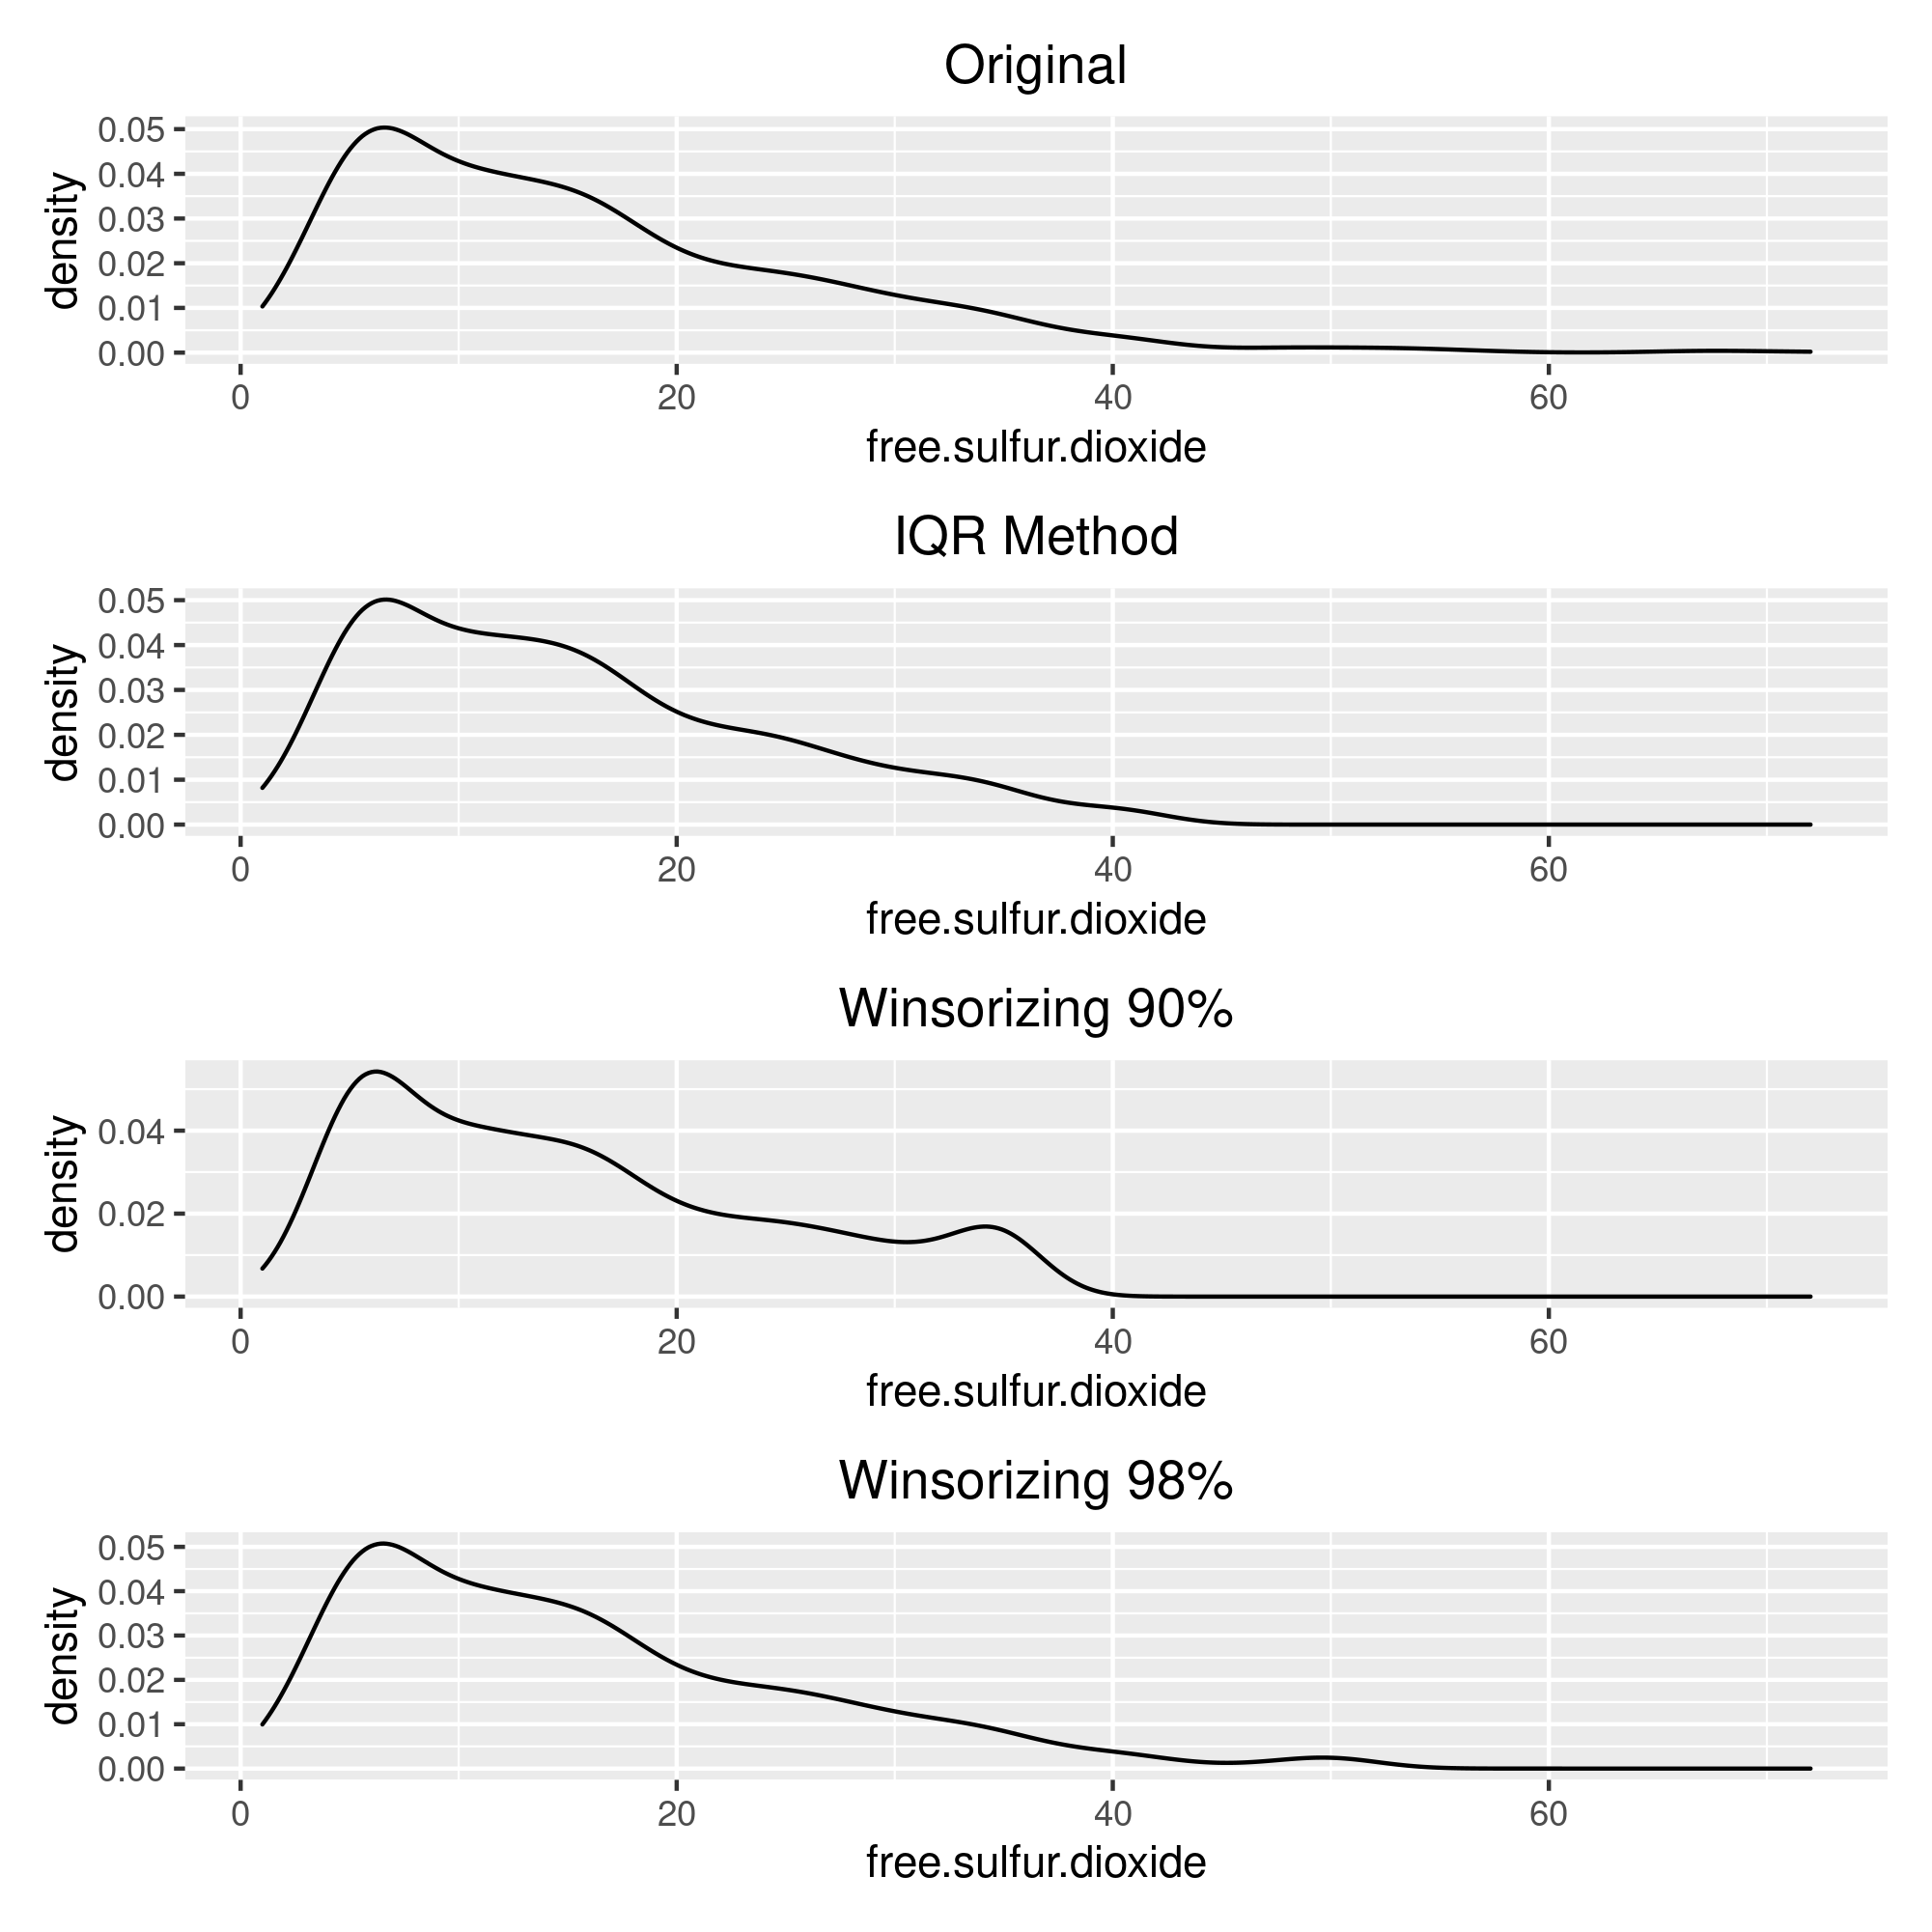
\includegraphics[width=0.45\textwidth]{images/outliers/free.sulfur.dioxide_distribution.png}
    }\qquad
    \subfloat[]{%
        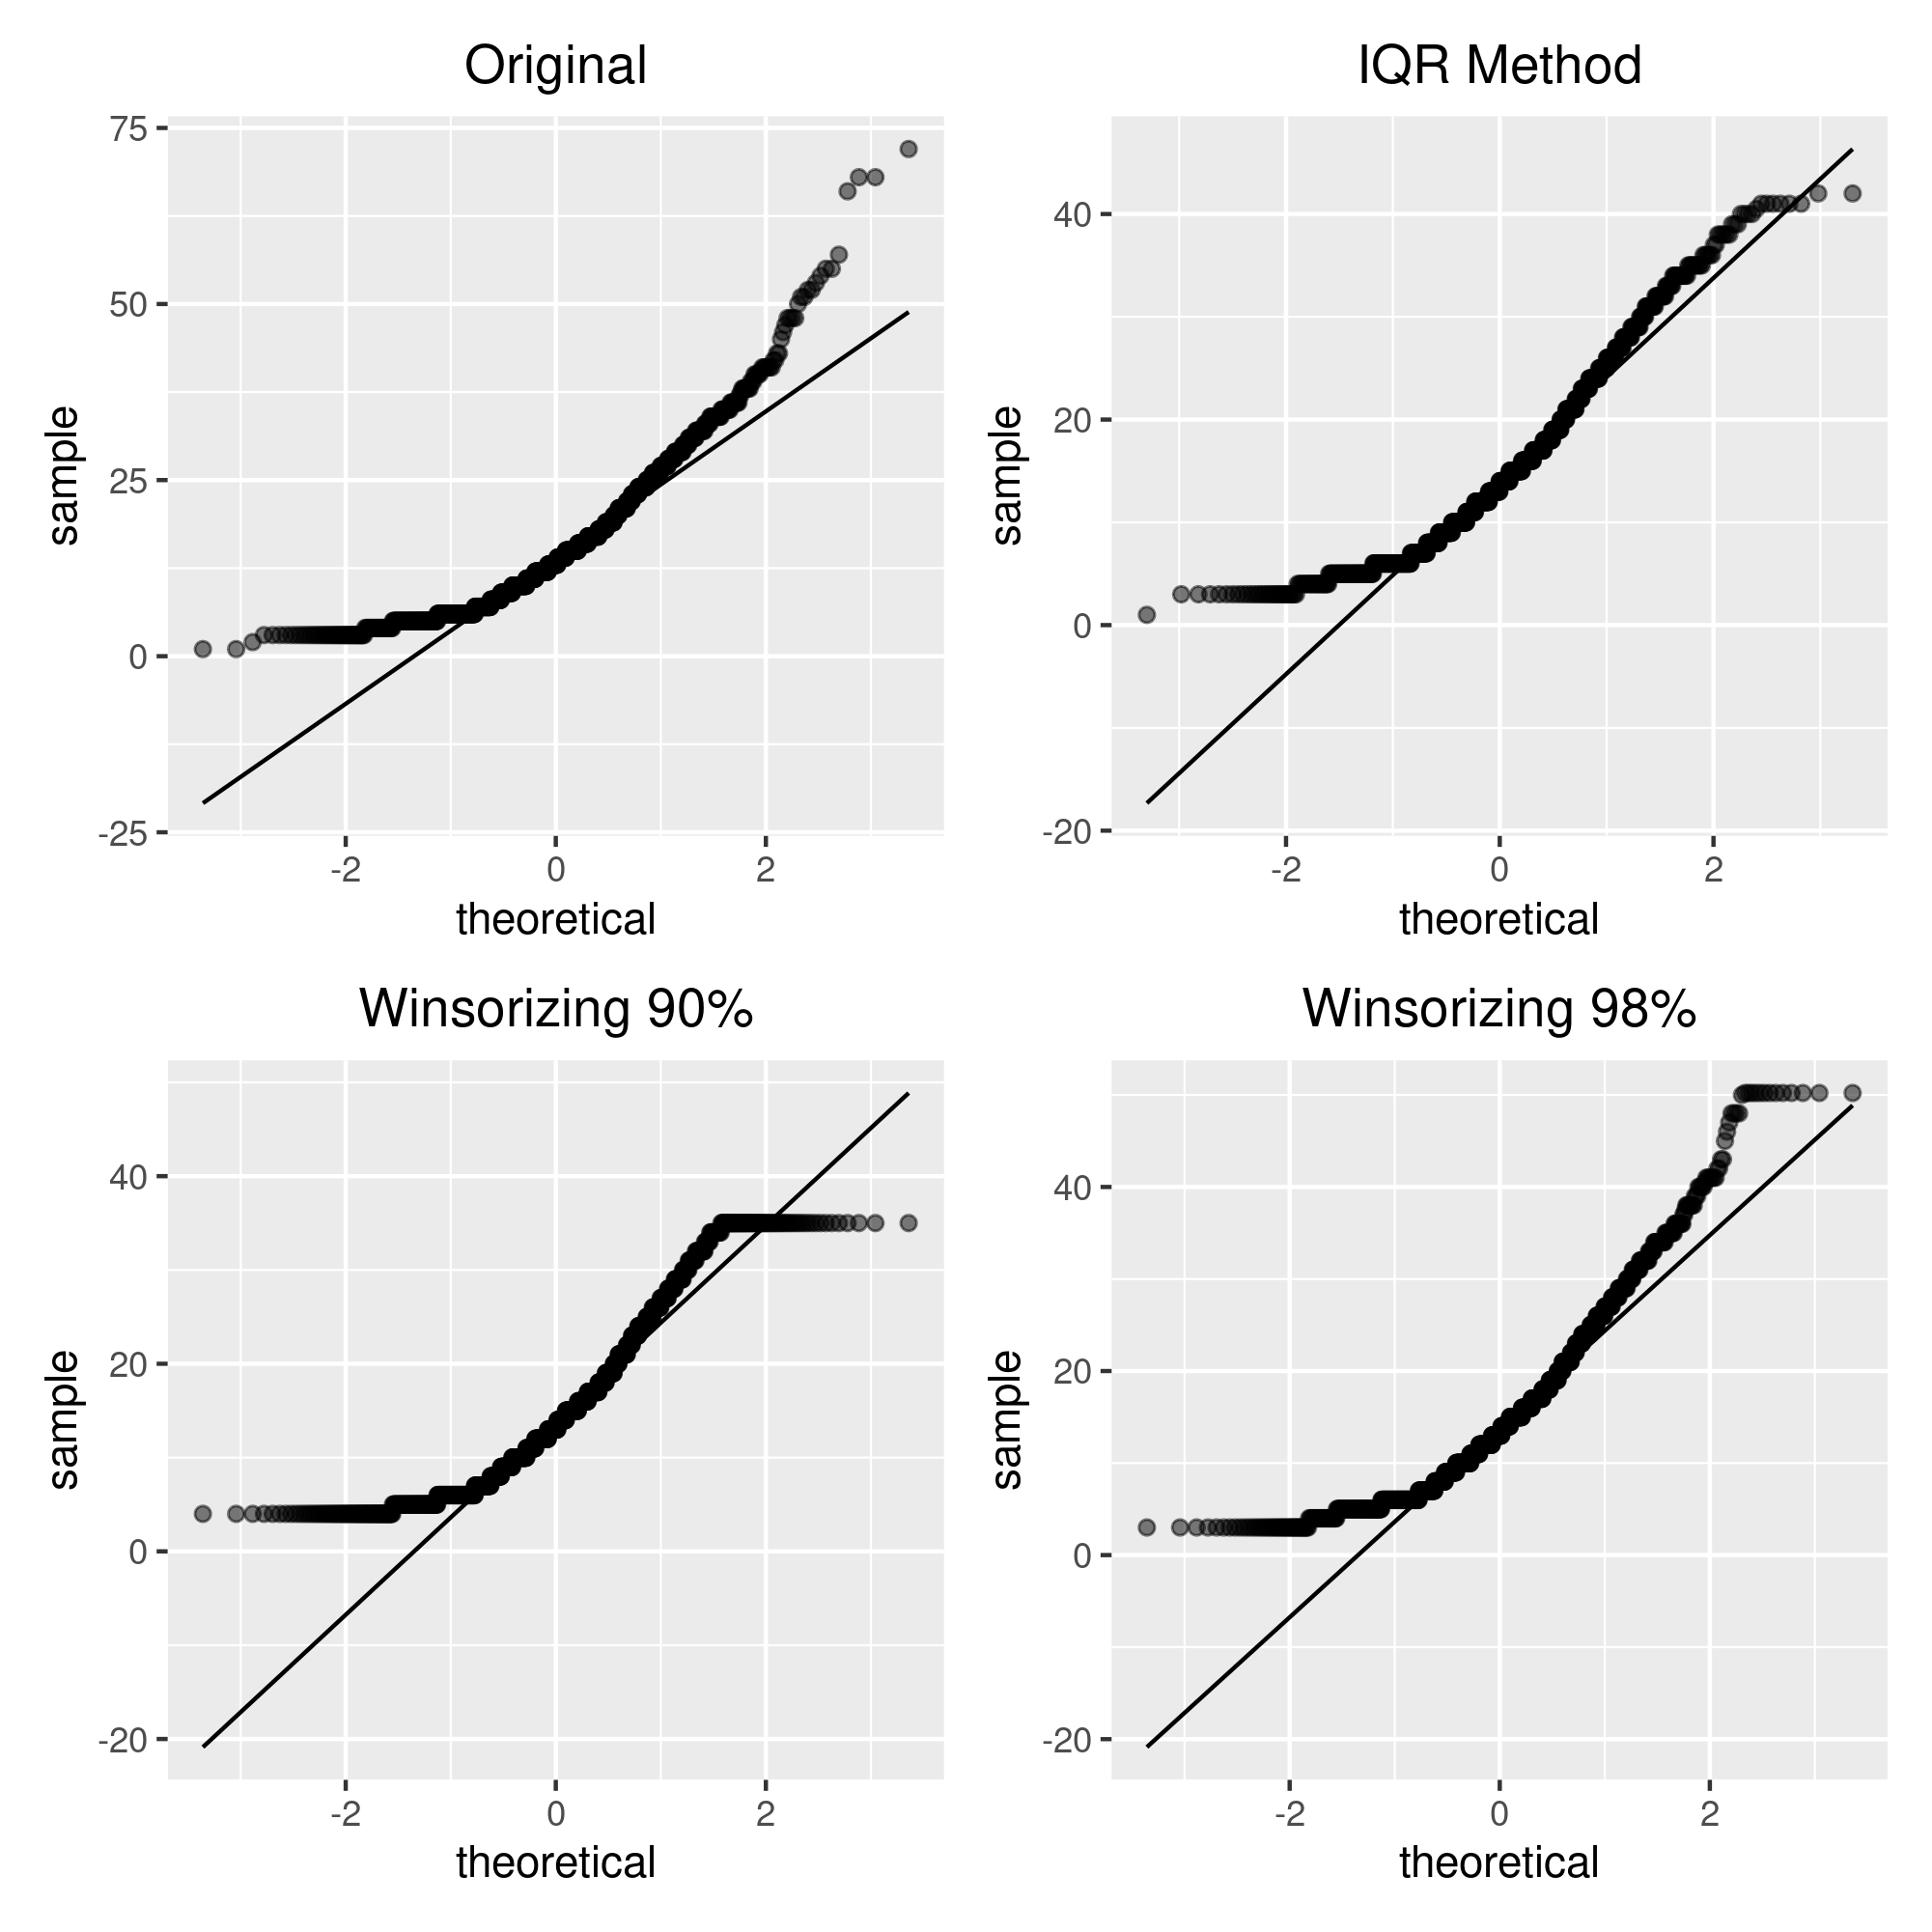
\includegraphics[width=0.45\textwidth]{images/outliers/free.sulfur.dioxide_qqplot.png}
    }

    \label{fig:outliers-free.sulfur.dioxide}
    \caption{Free Sulfur Dioxide}
\end{figure}

\begin{figure}[H]
    \centering

    \subfloat[]{%
        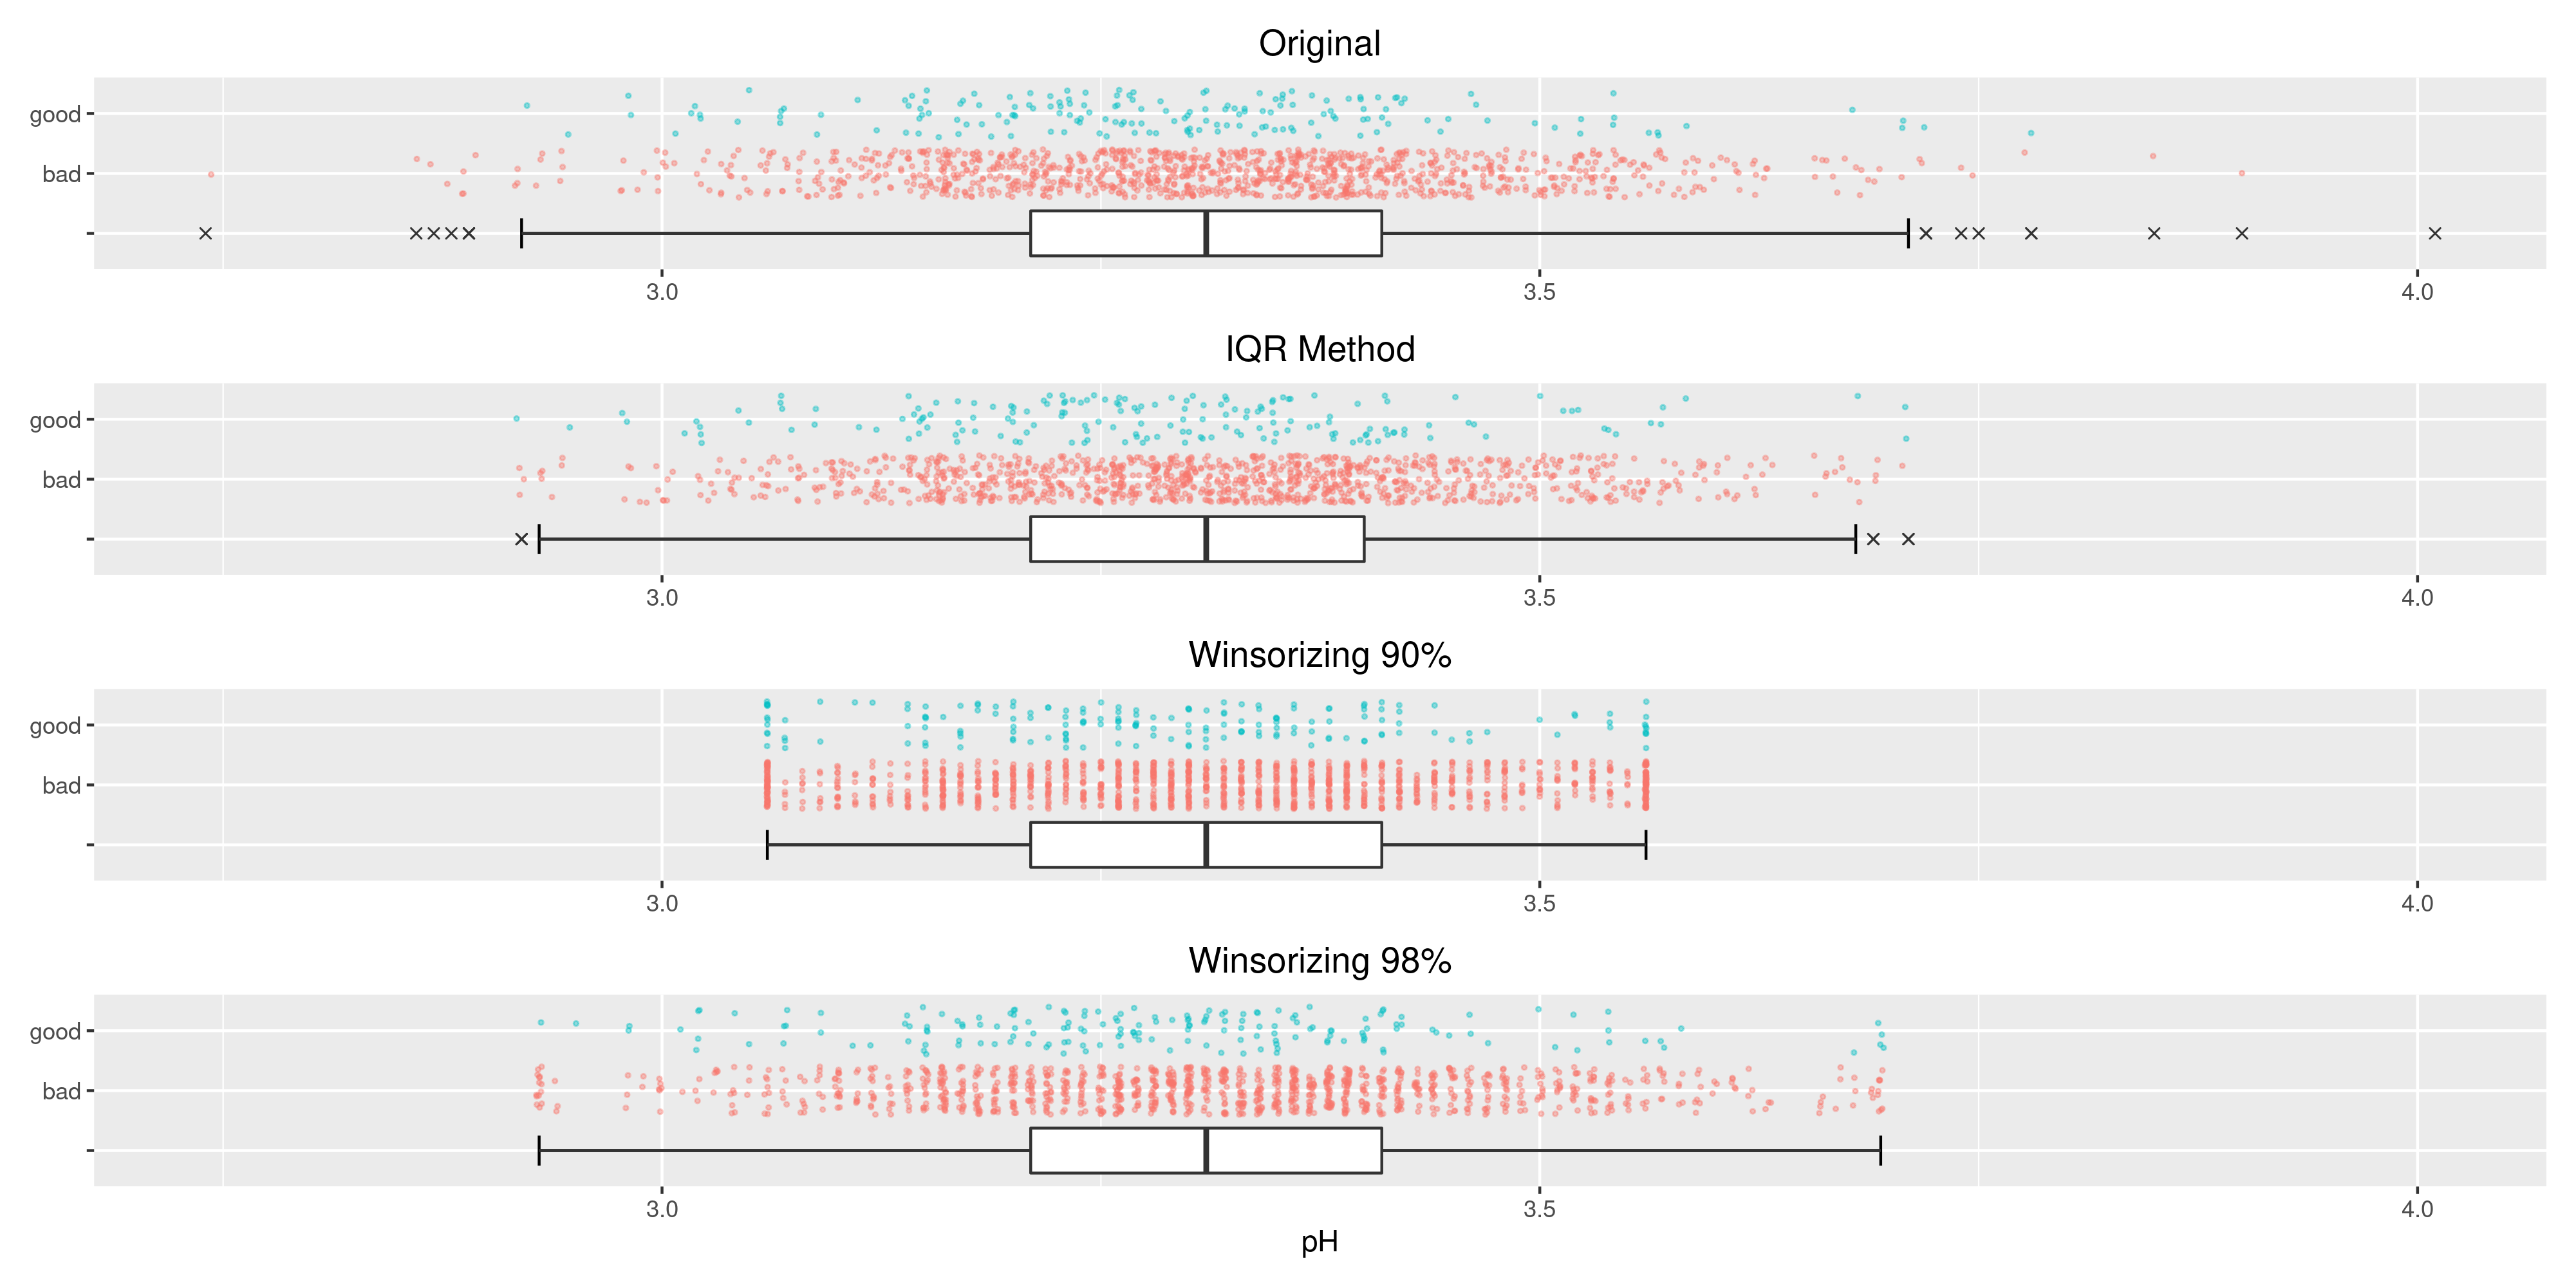
\includegraphics[width=0.99\textwidth]{images/outliers/pH_boxplot.png}
    }

    \subfloat[]{%
        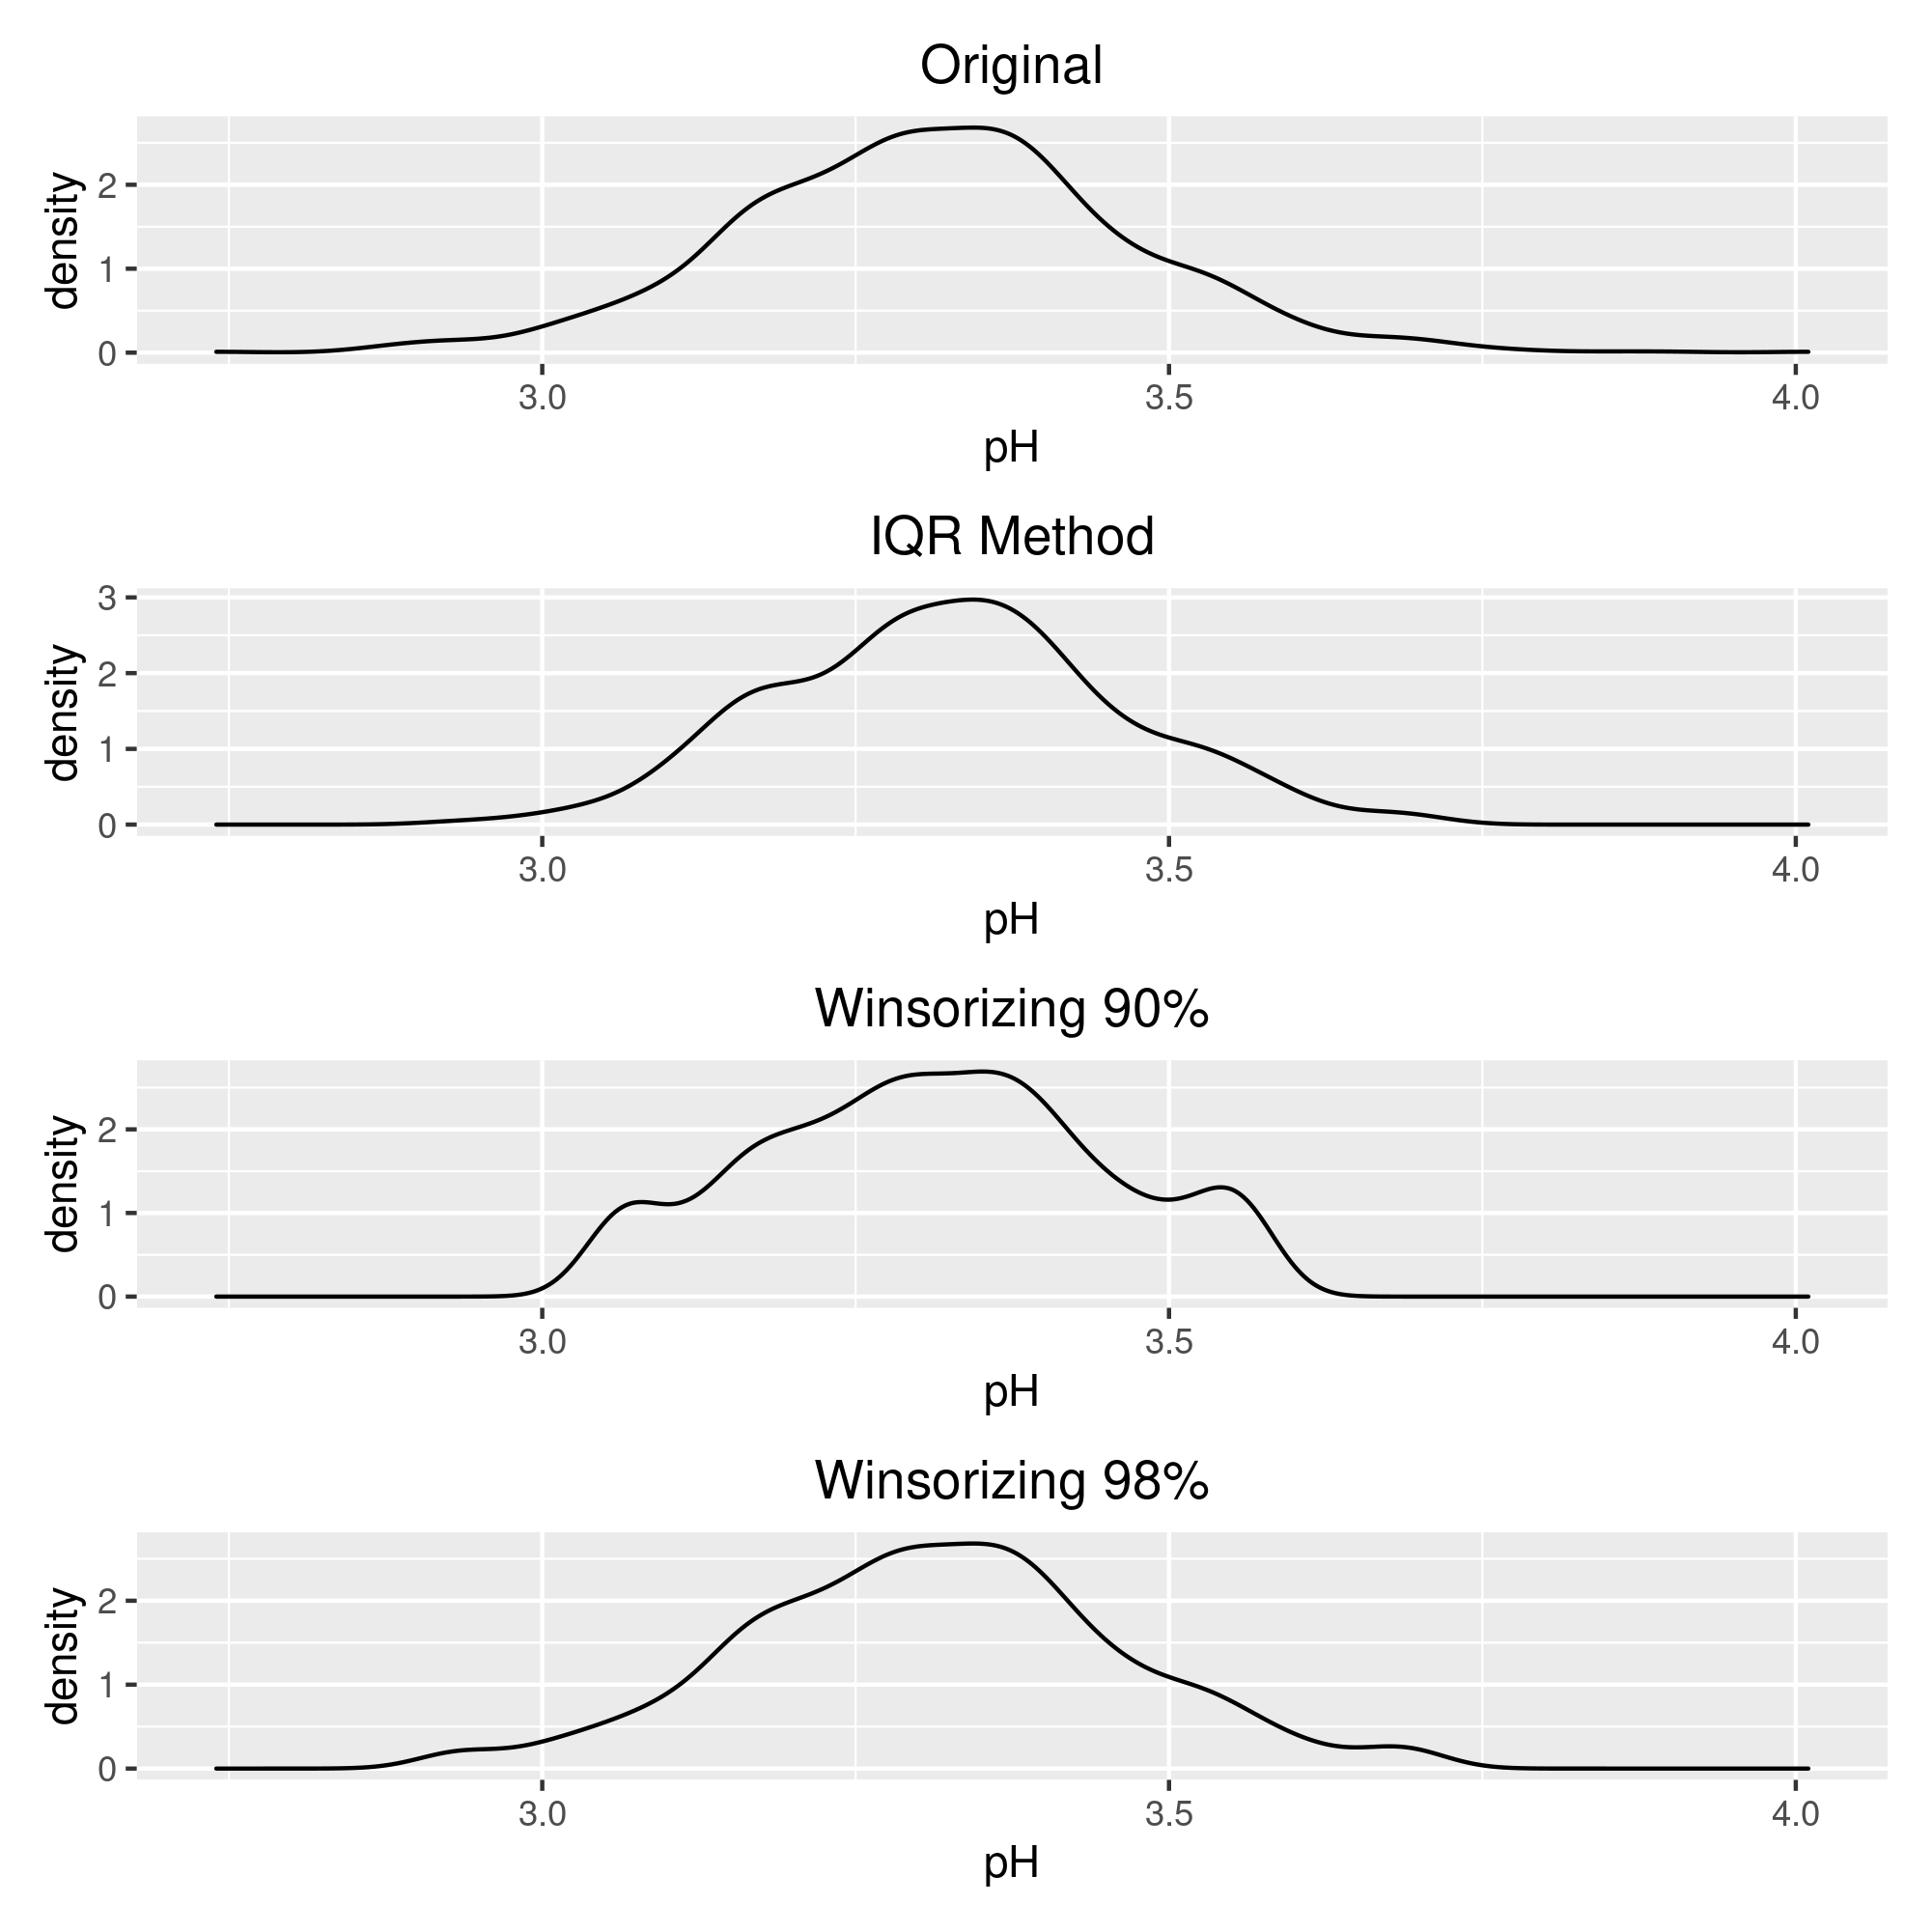
\includegraphics[width=0.45\textwidth]{images/outliers/pH_distribution.png}
    }\qquad
    \subfloat[]{%
        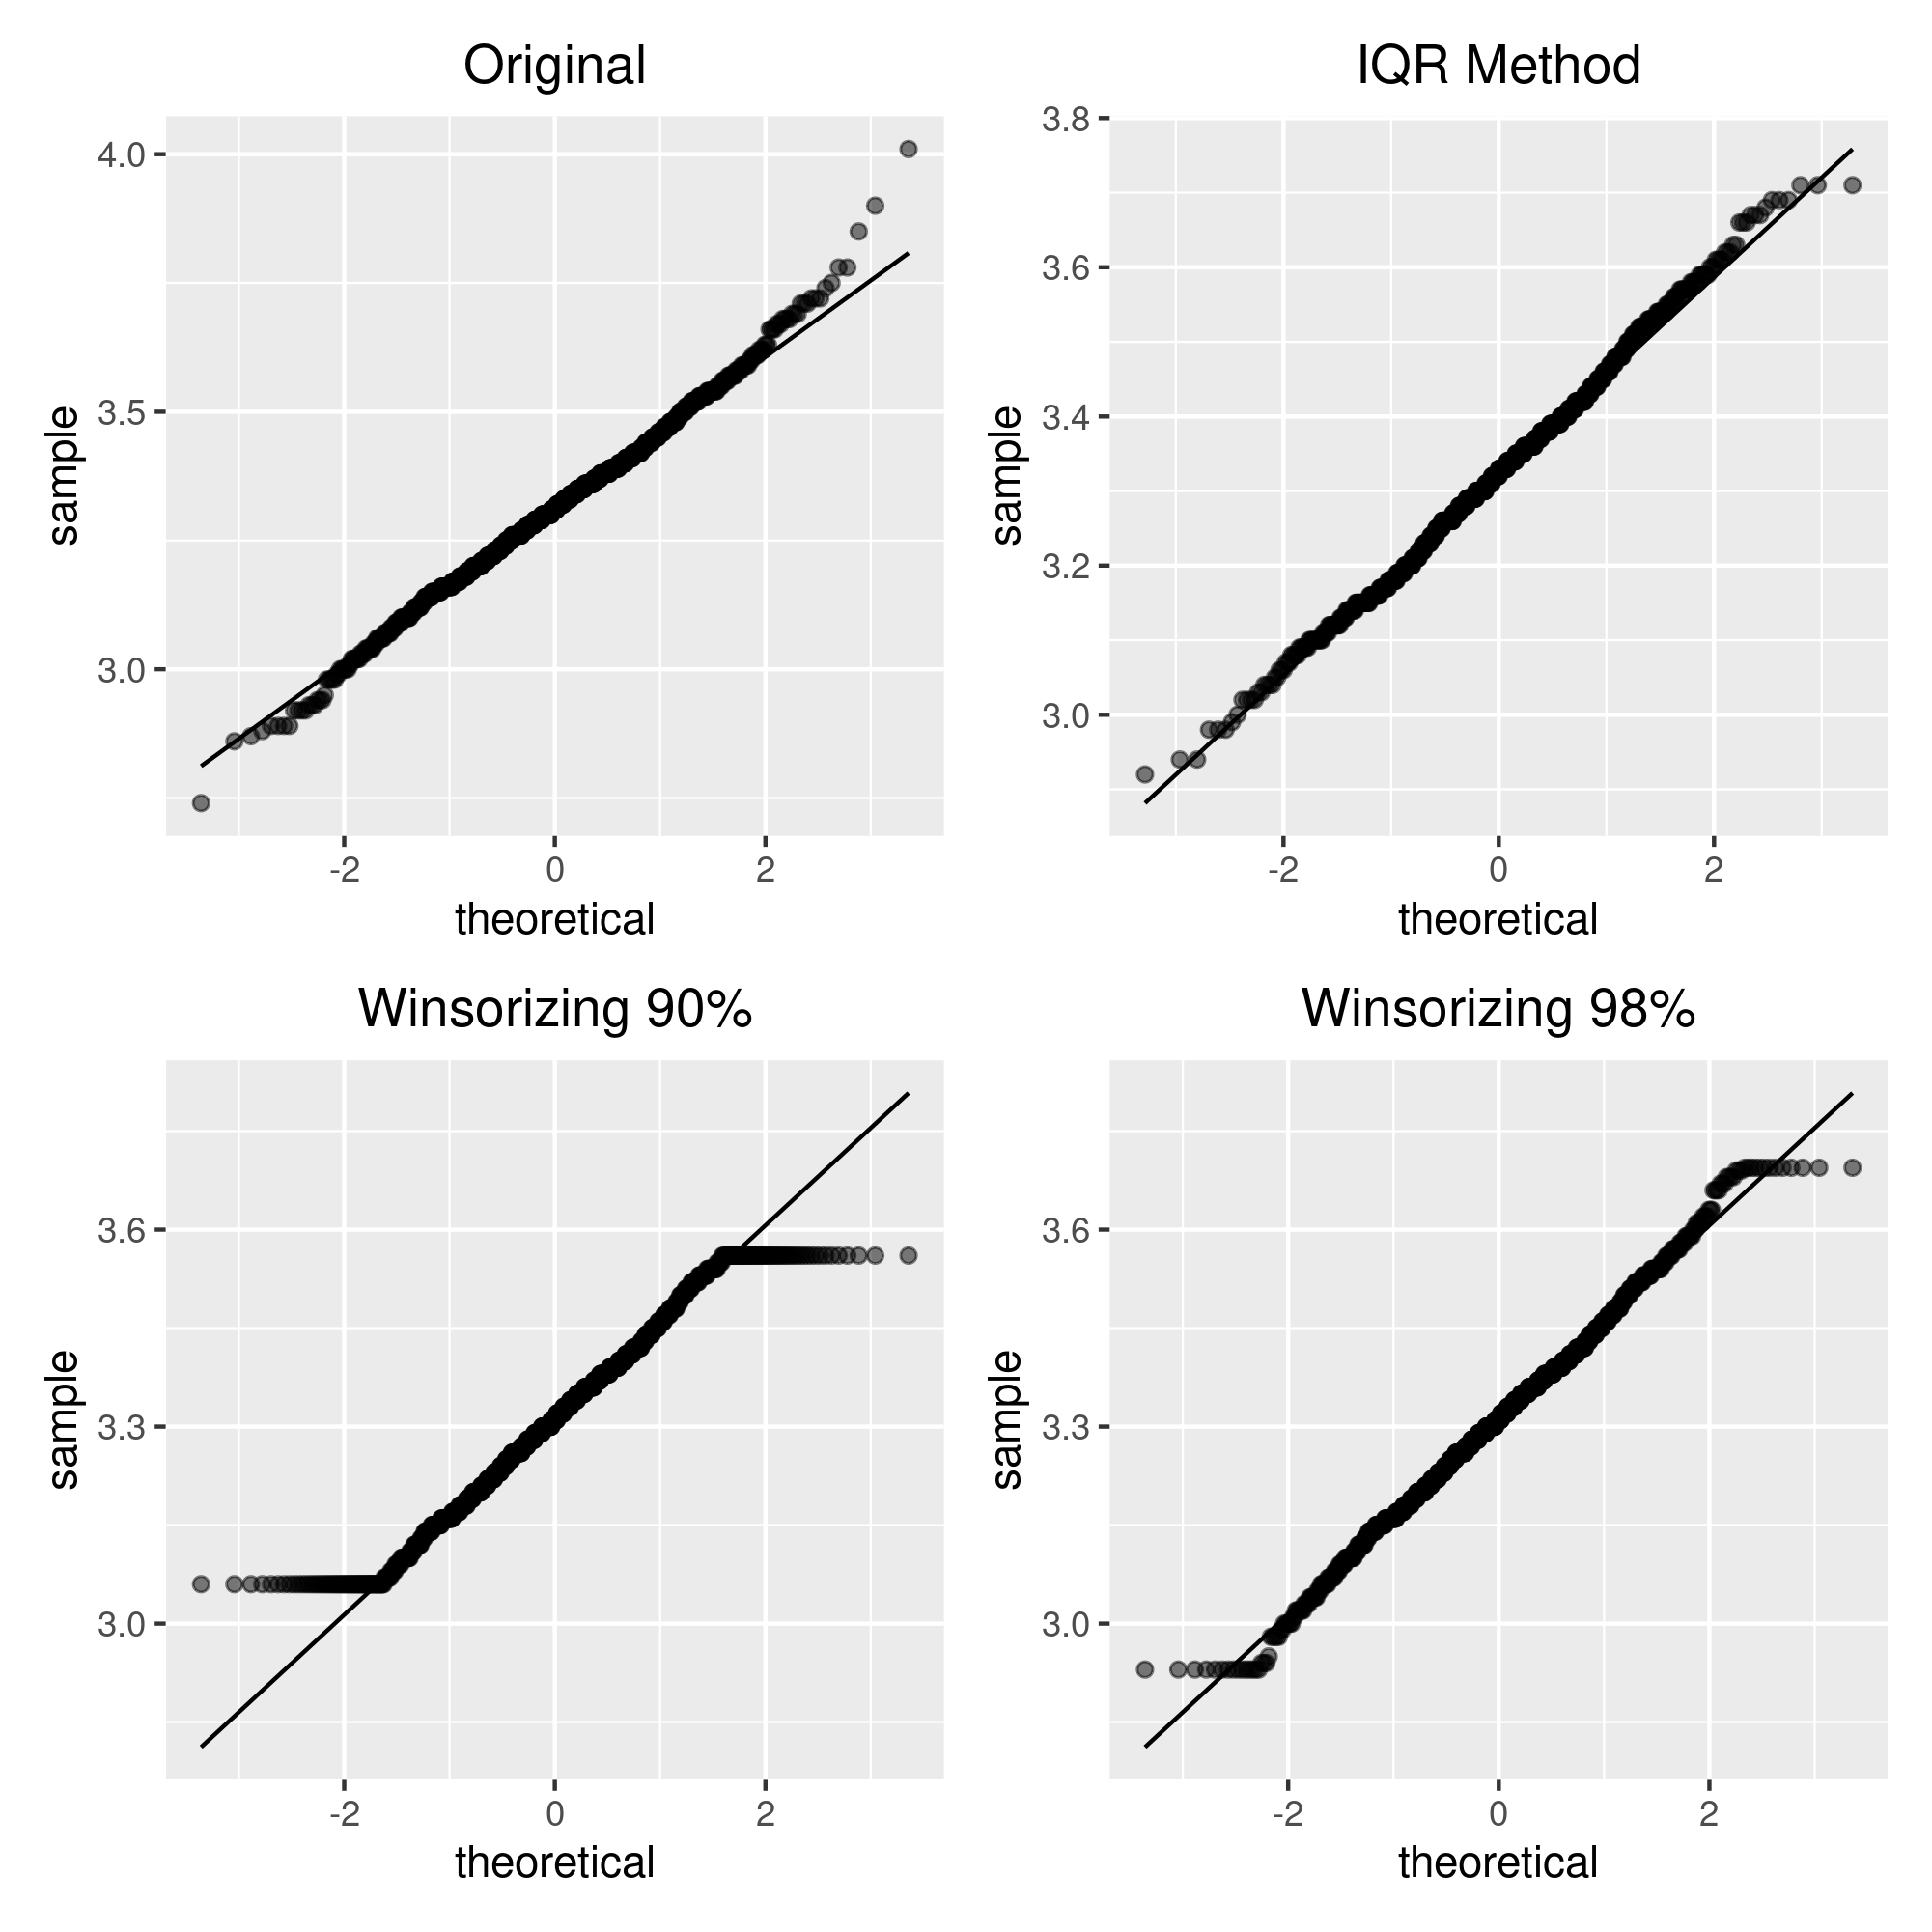
\includegraphics[width=0.45\textwidth]{images/outliers/pH_qqplot.png}
    }

    \label{fig:outliers-pH}
    \caption{PH}
\end{figure}

\begin{figure}[H]
    \centering

    \subfloat[]{%
        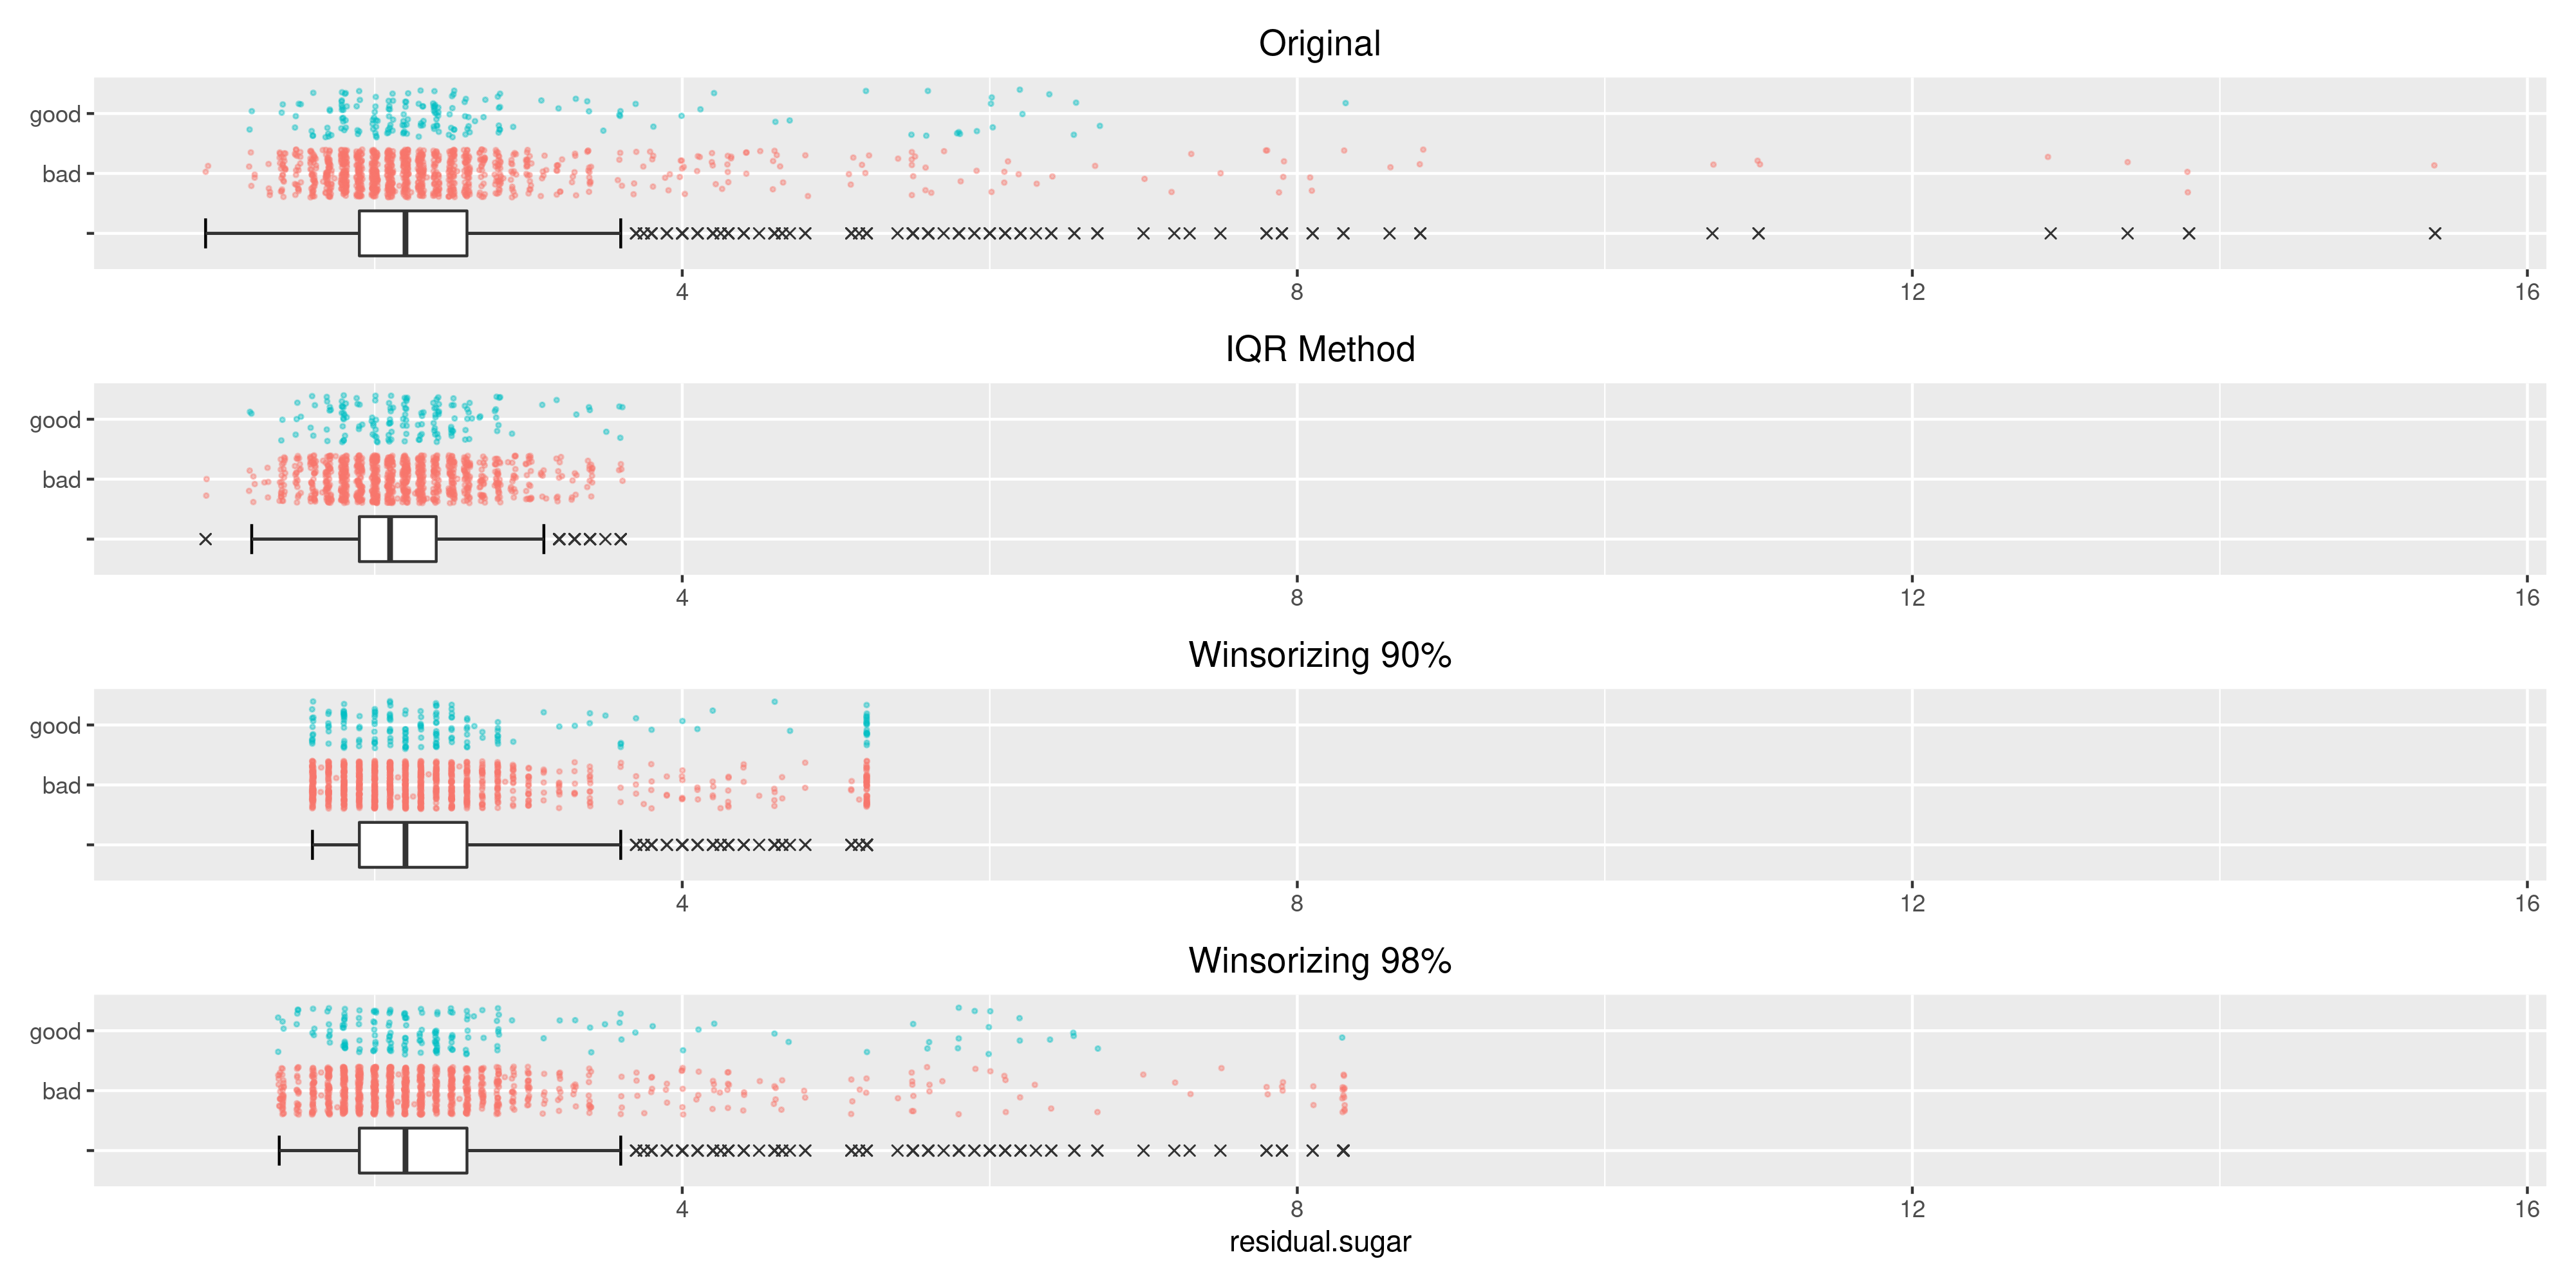
\includegraphics[width=0.99\textwidth]{images/outliers/residual.sugar_boxplot.png}
    }

    \subfloat[]{%
        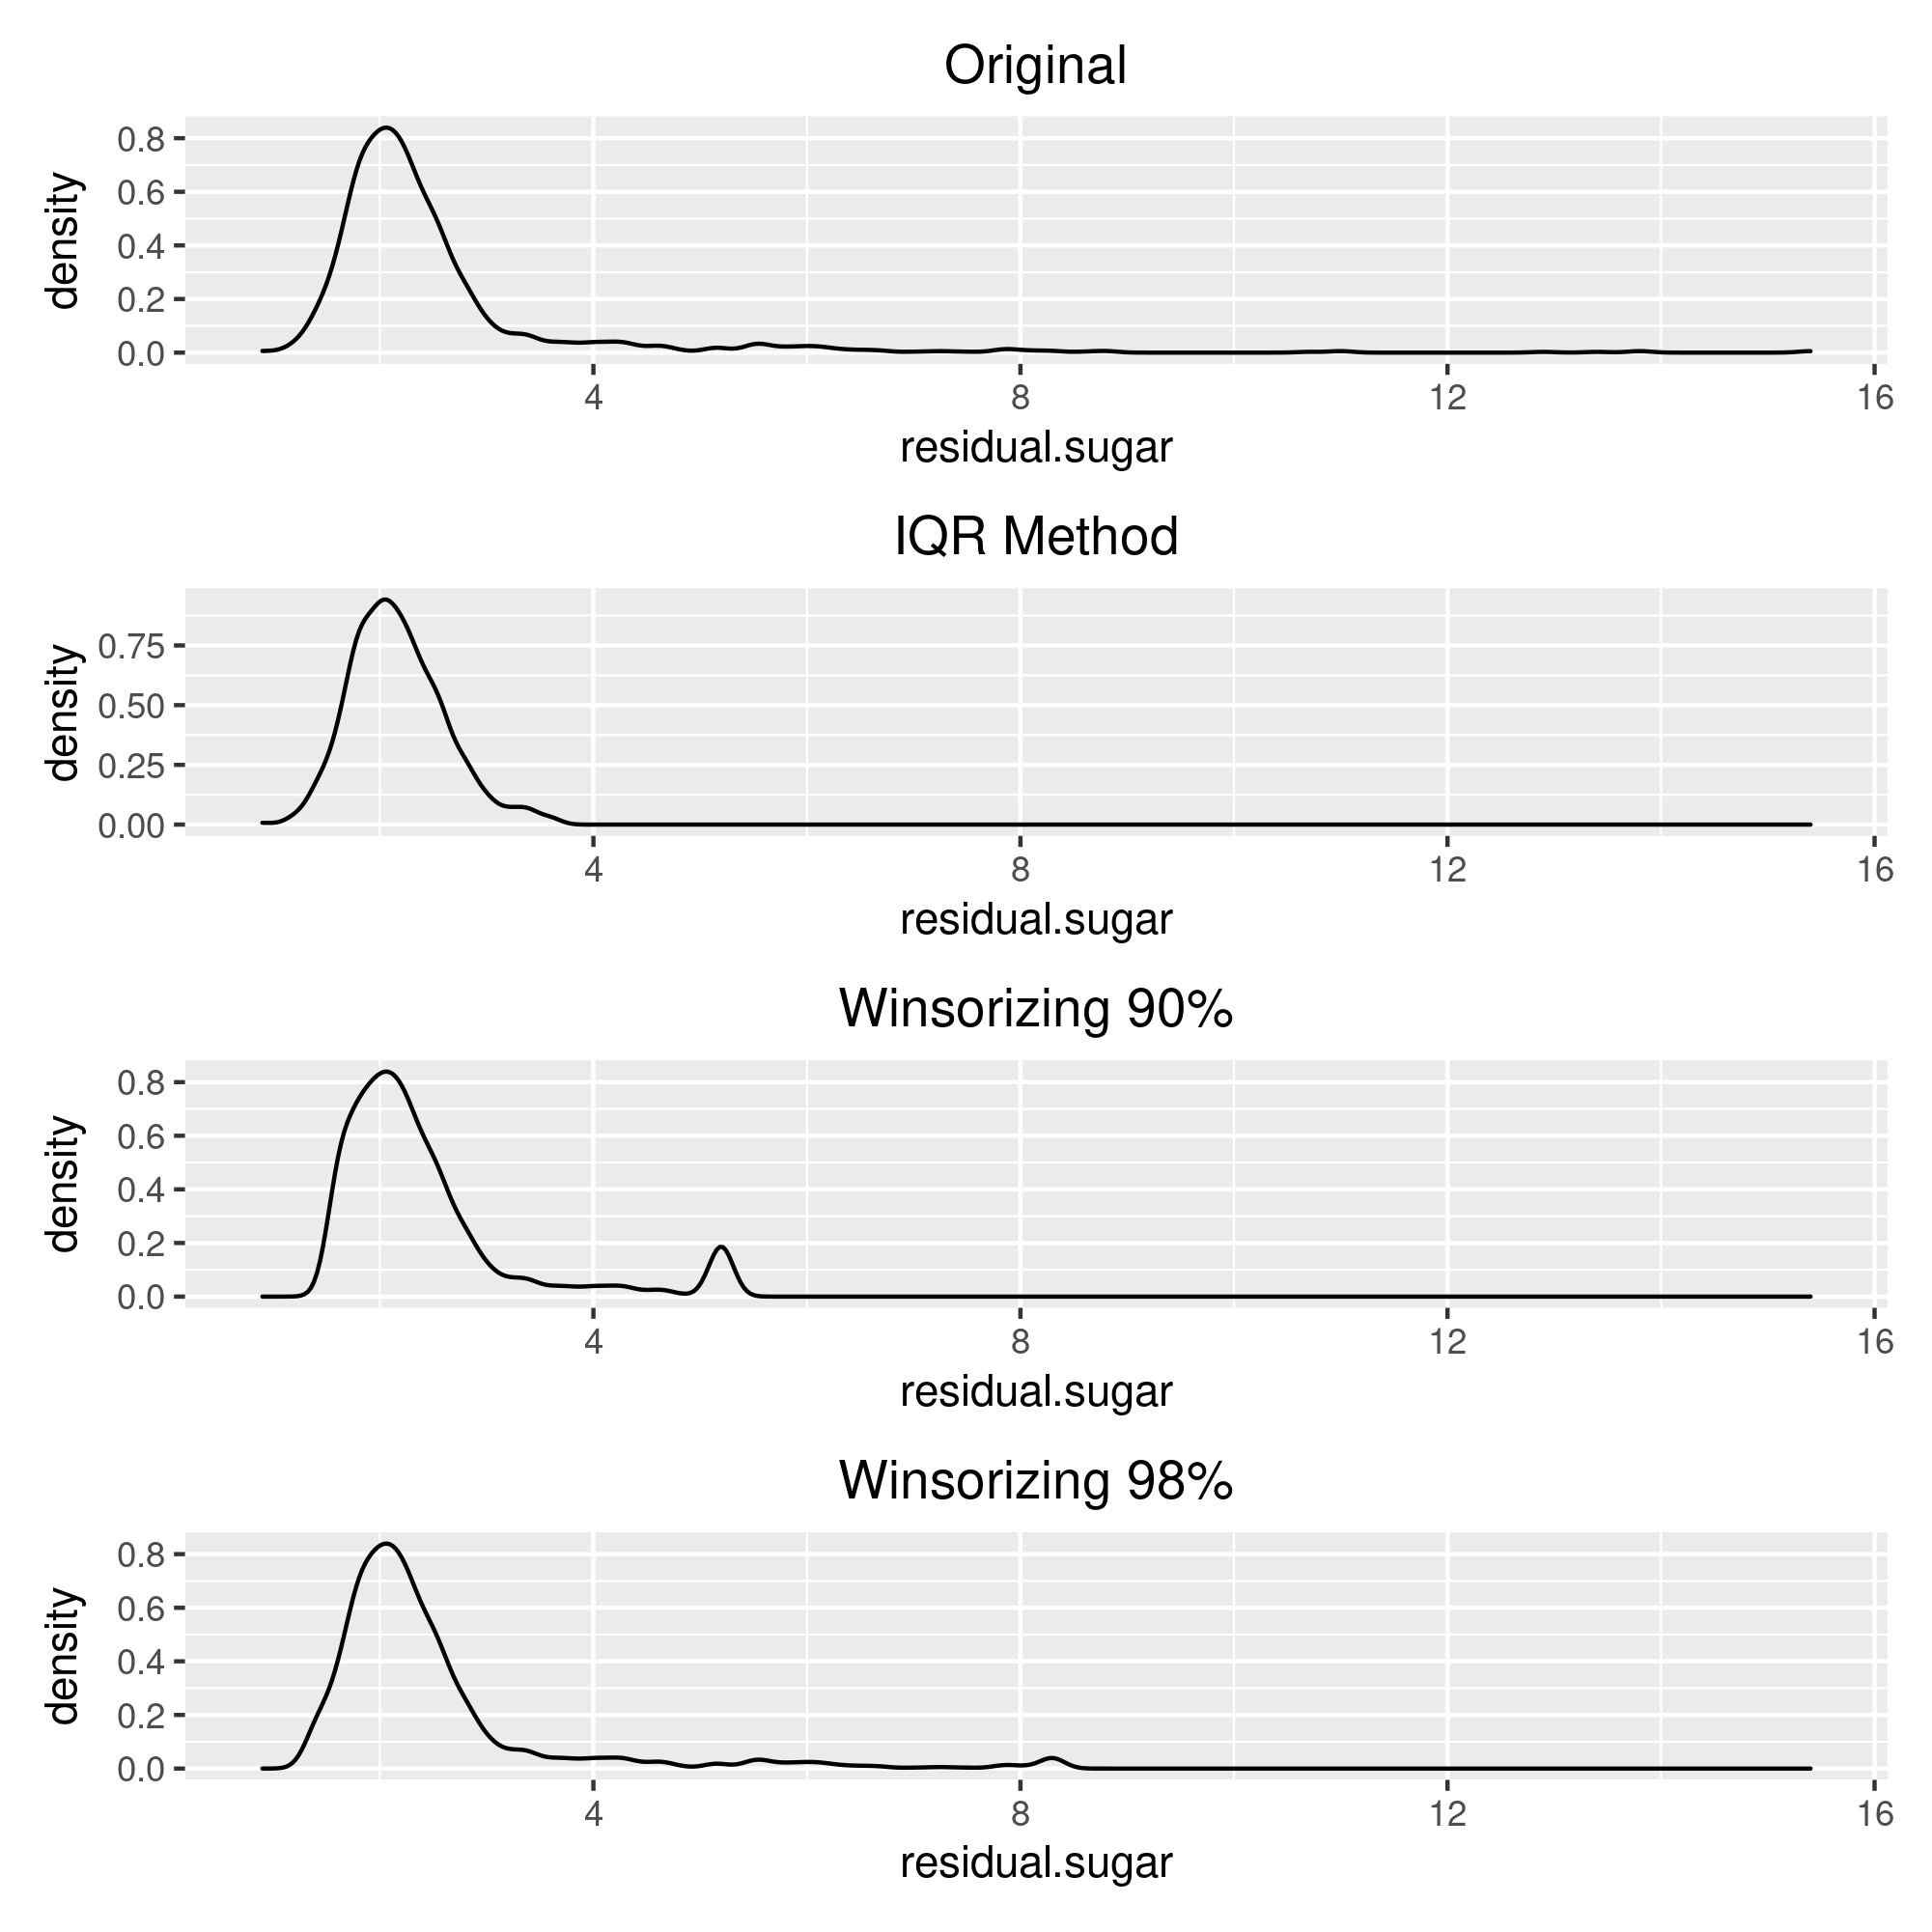
\includegraphics[width=0.45\textwidth]{images/outliers/residual.sugar_distribution.png}
    }\qquad
    \subfloat[]{%
        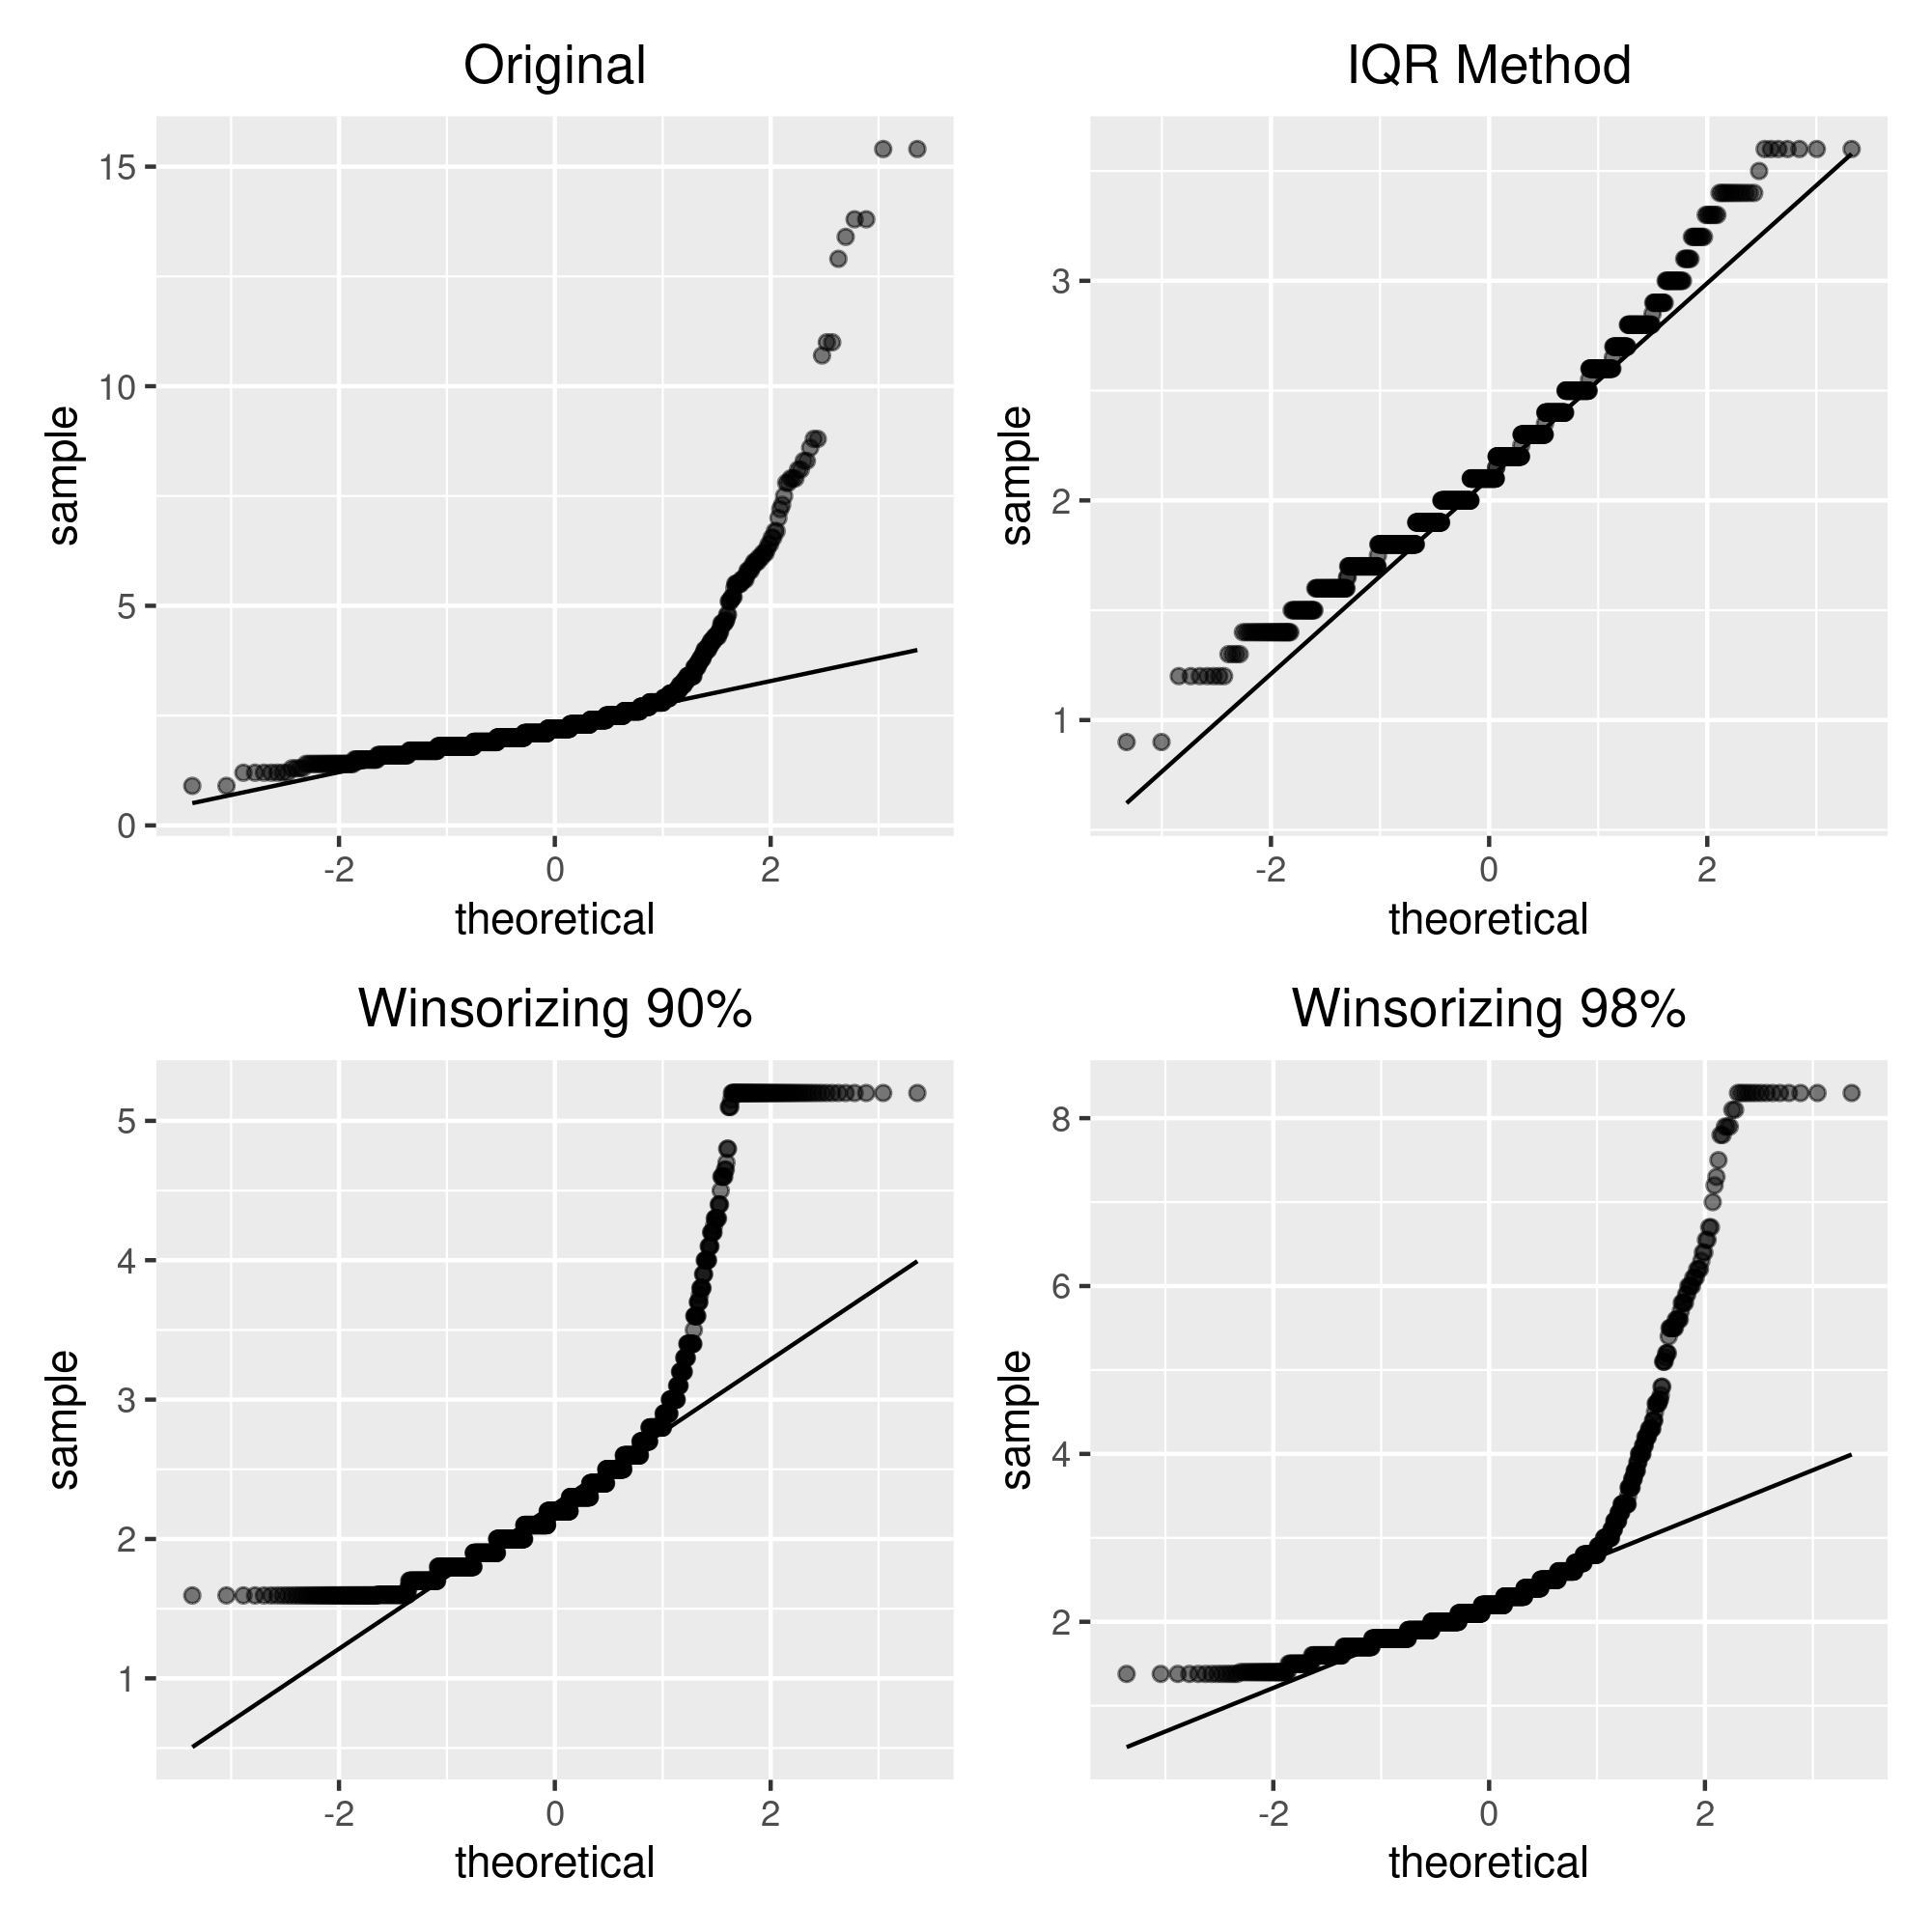
\includegraphics[width=0.45\textwidth]{images/outliers/residual.sugar_qqplot.png}
    }

    \label{fig:outliers-residual.sugar}
    \caption{Residual Sugar}
\end{figure}

\begin{figure}[H]
    \centering

    \subfloat[]{%
        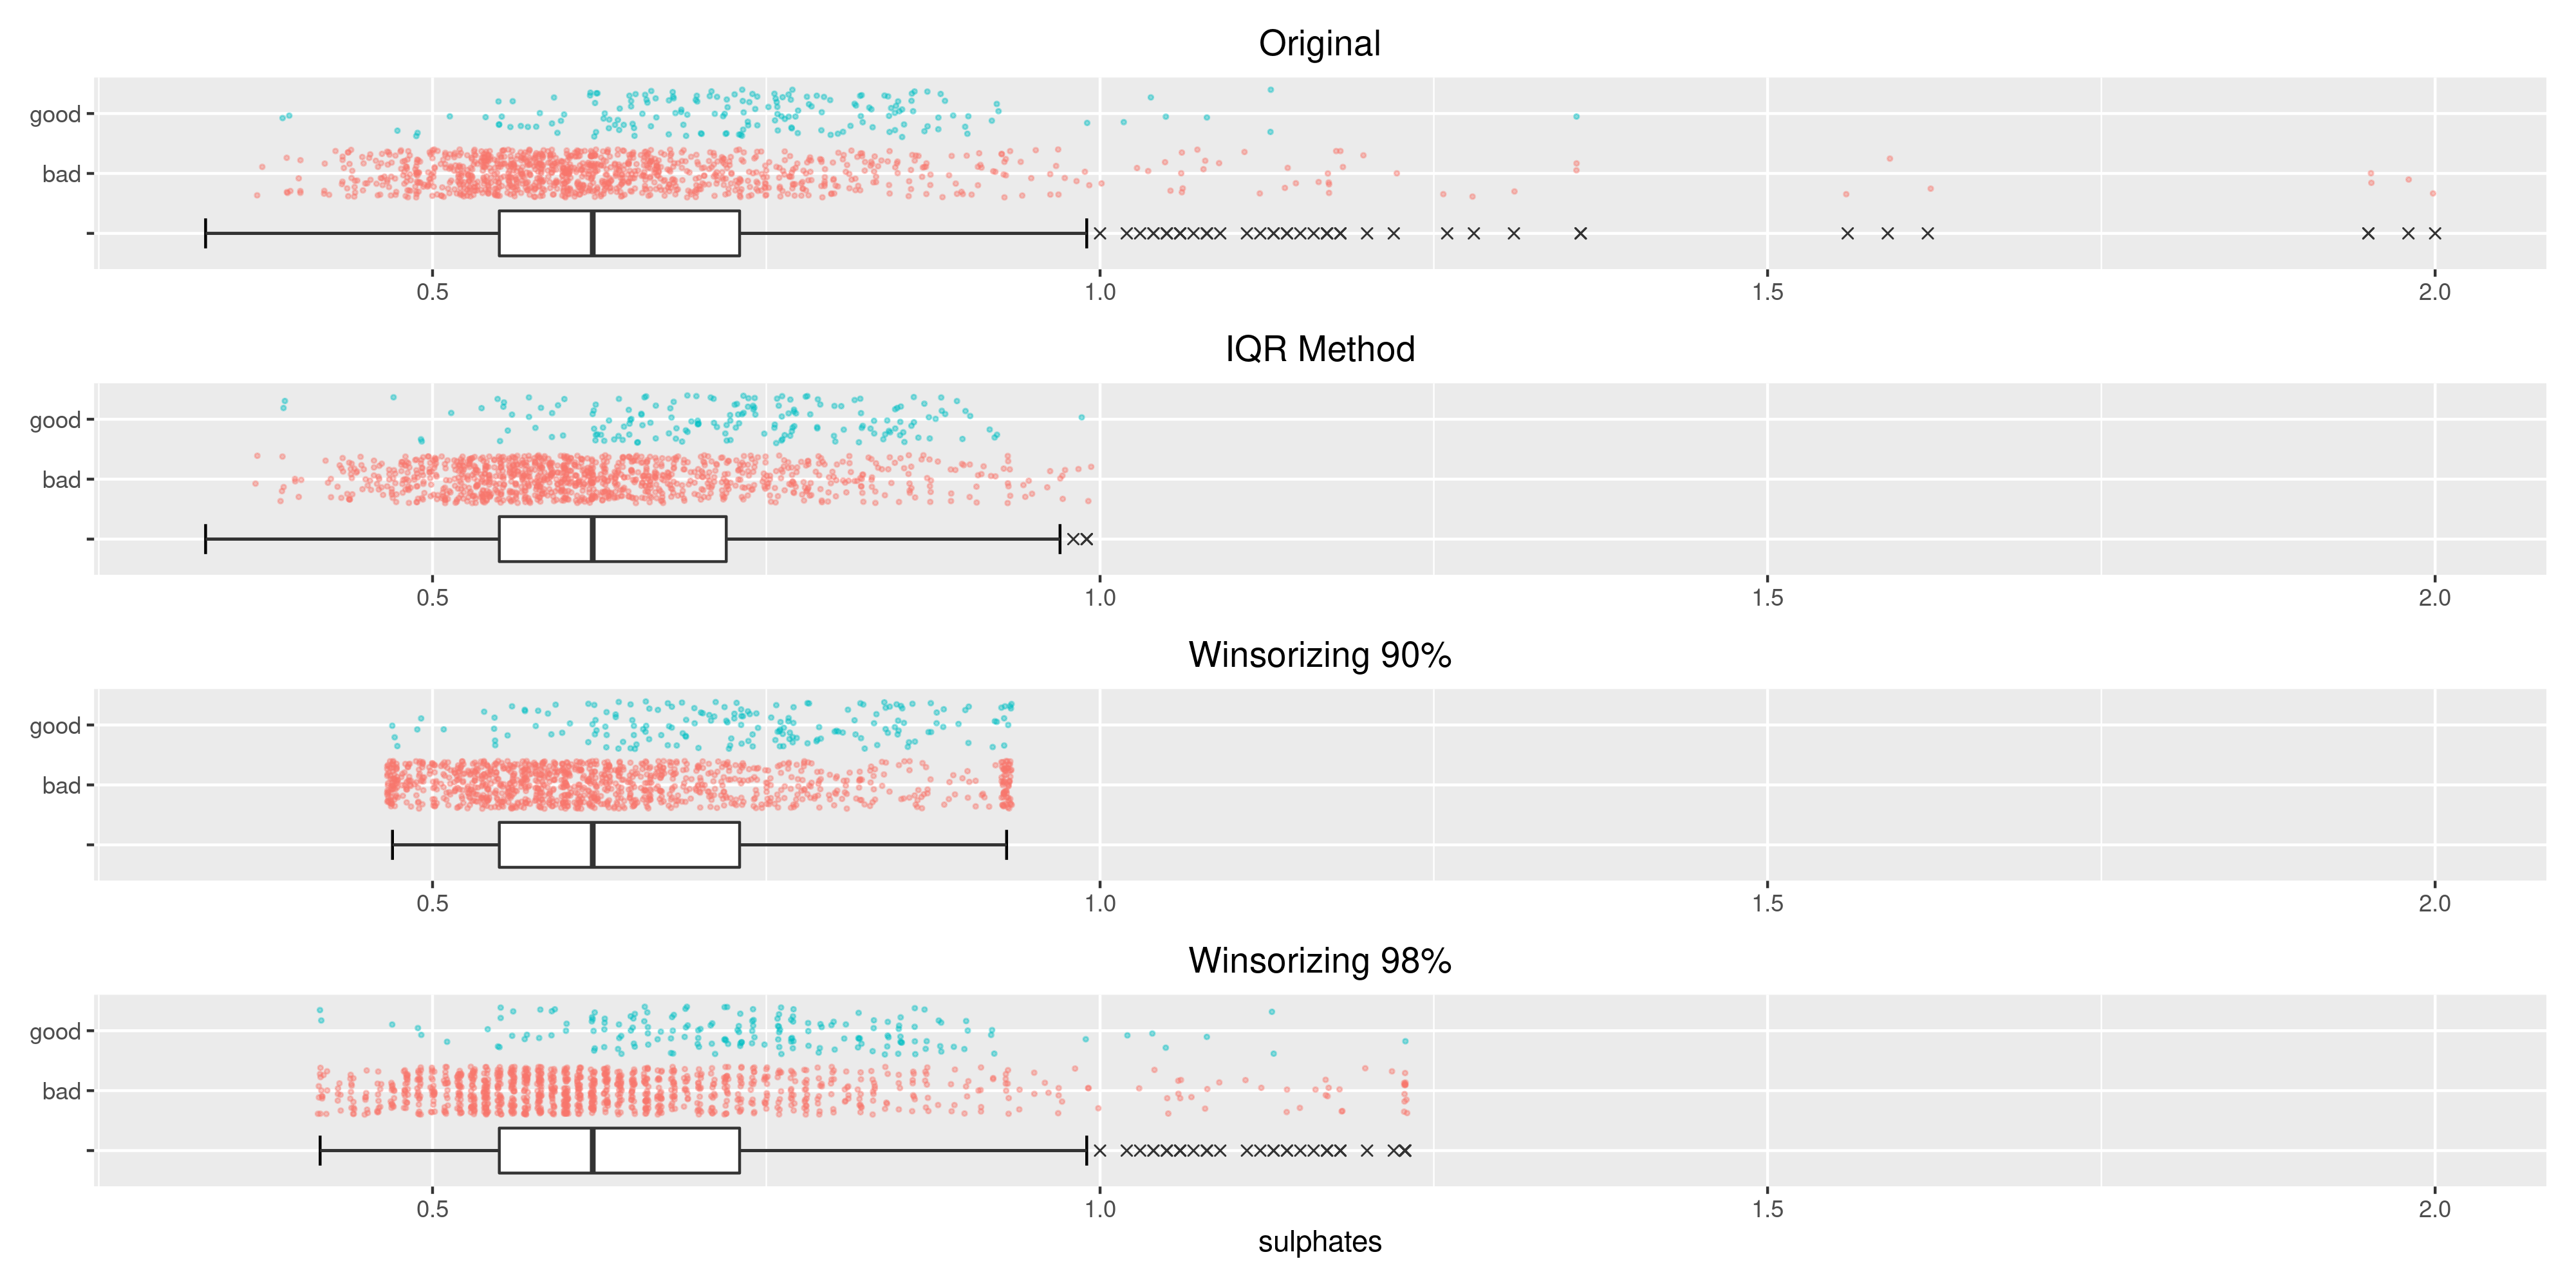
\includegraphics[width=0.99\textwidth]{images/outliers/sulphates_boxplot.png}
    }

    \subfloat[]{%
        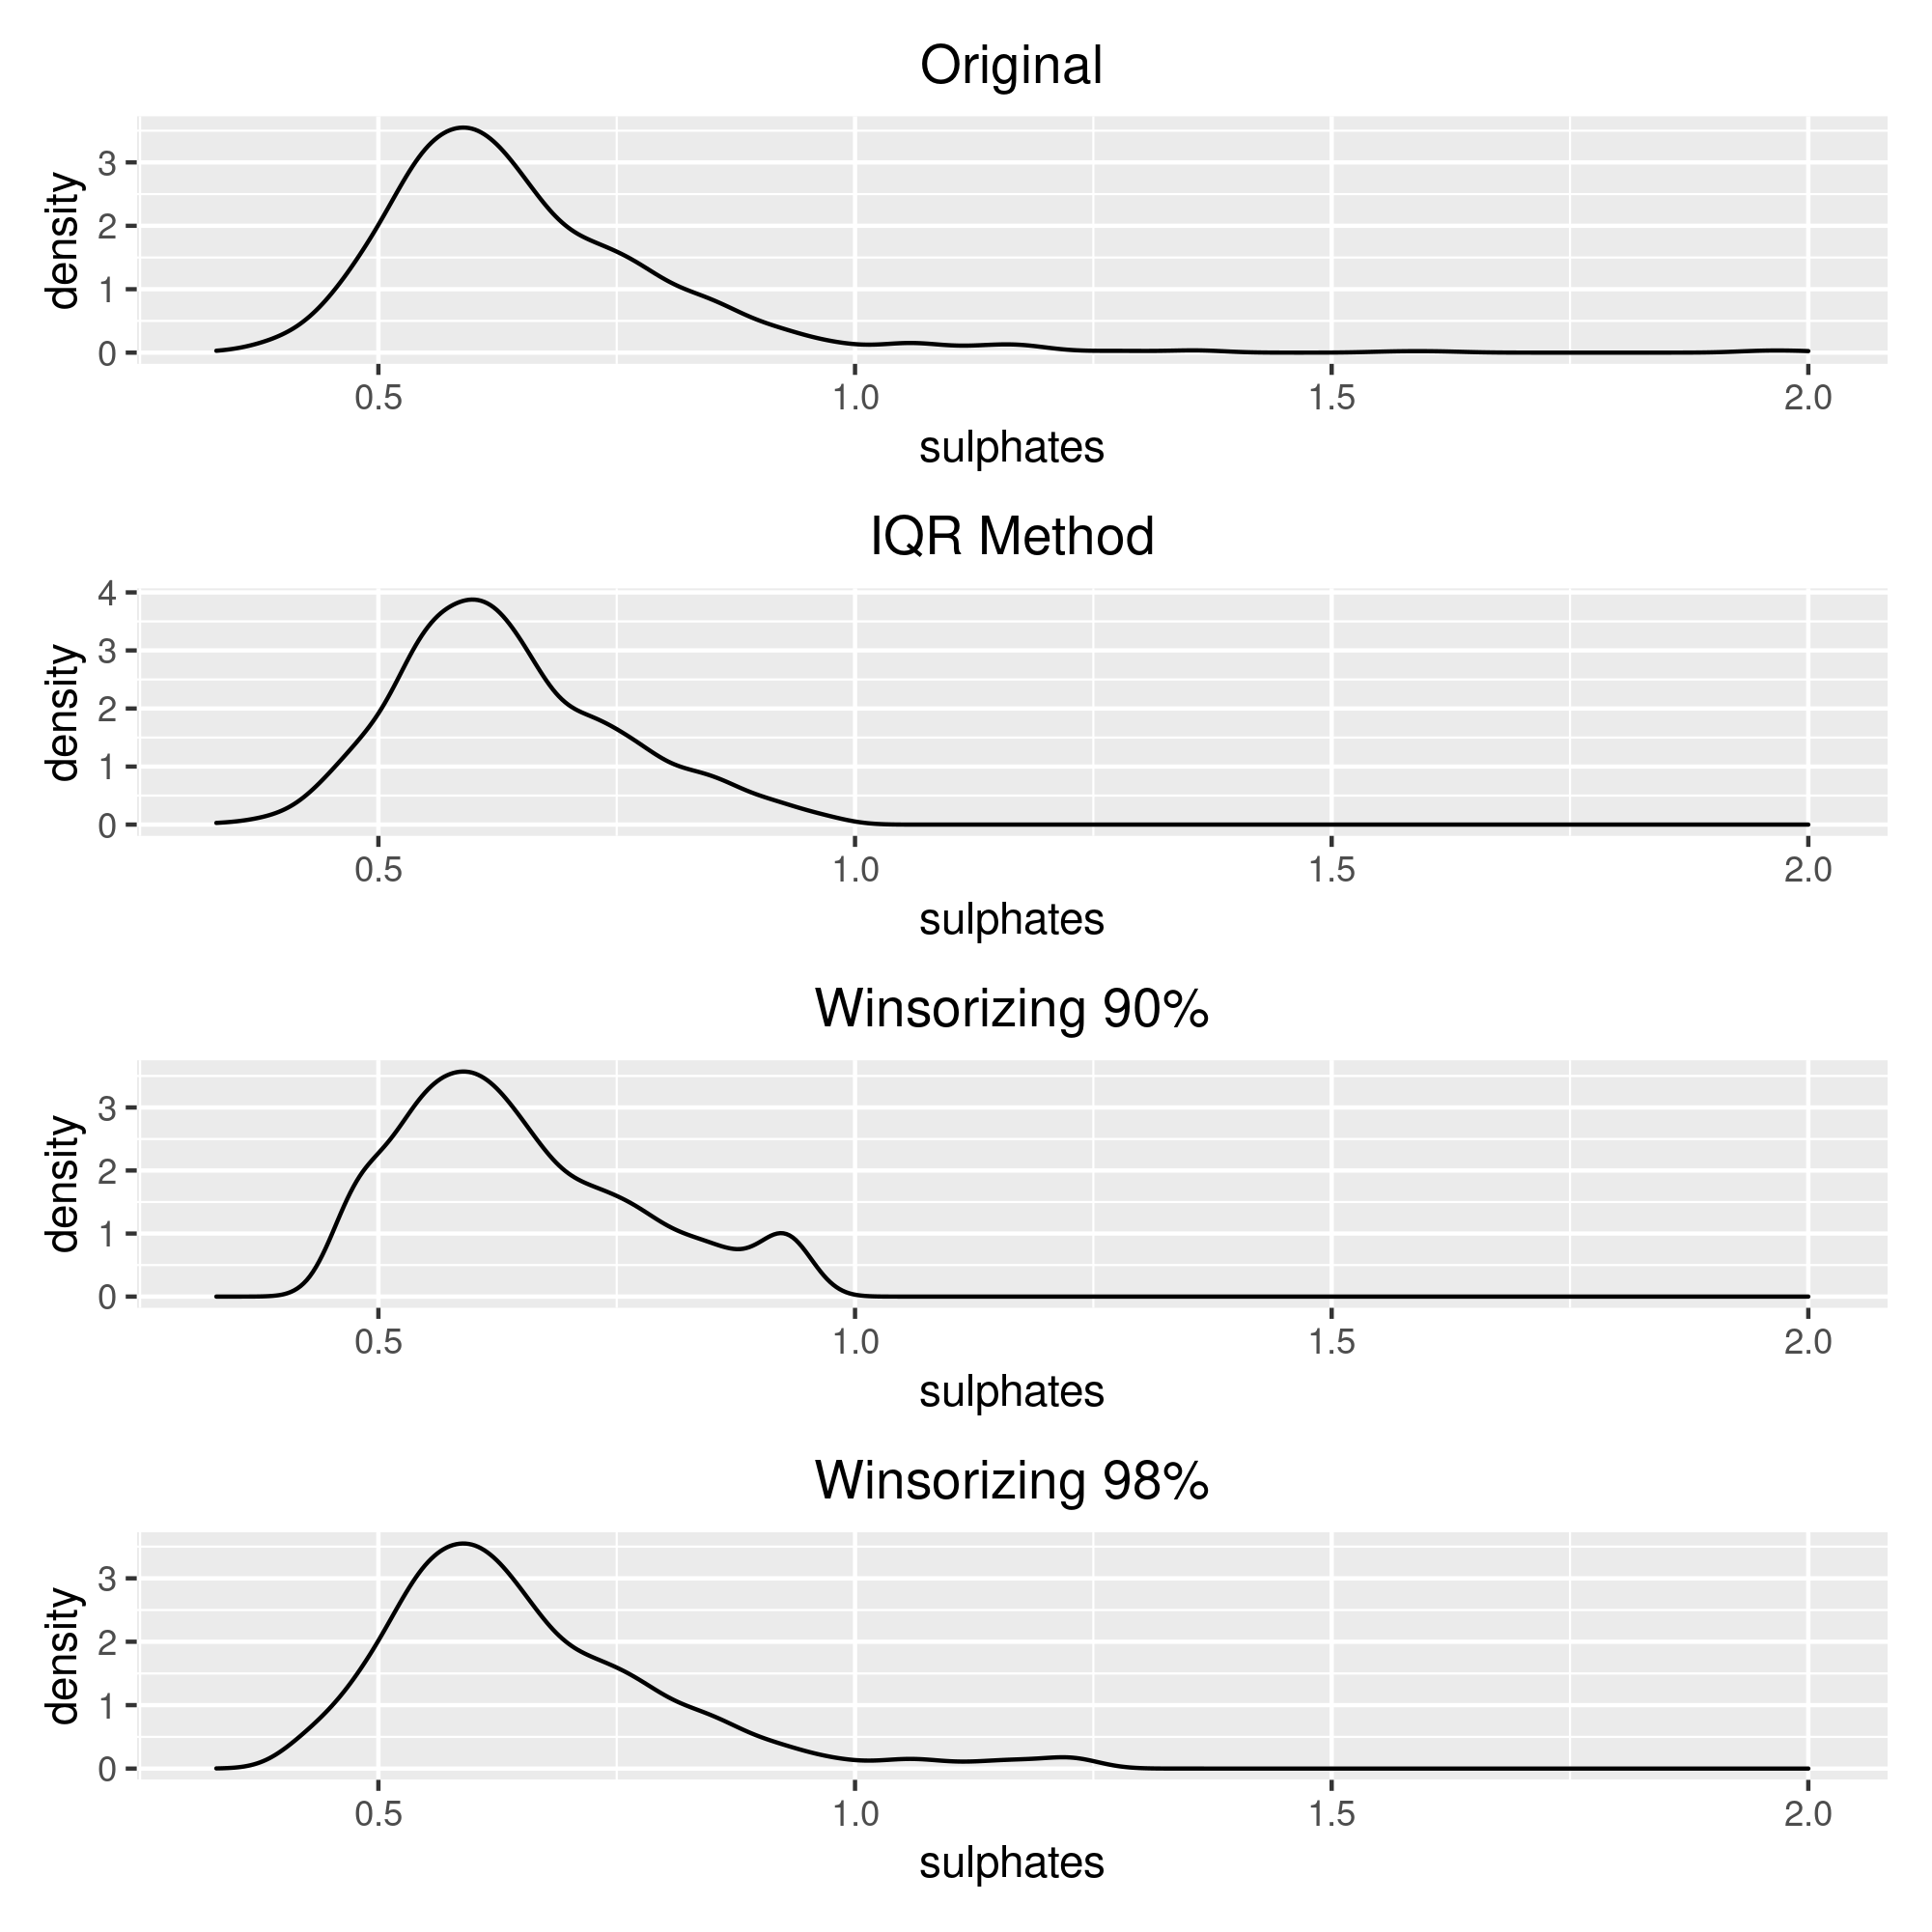
\includegraphics[width=0.45\textwidth]{images/outliers/sulphates_distribution.png}
    }\qquad
    \subfloat[]{%
        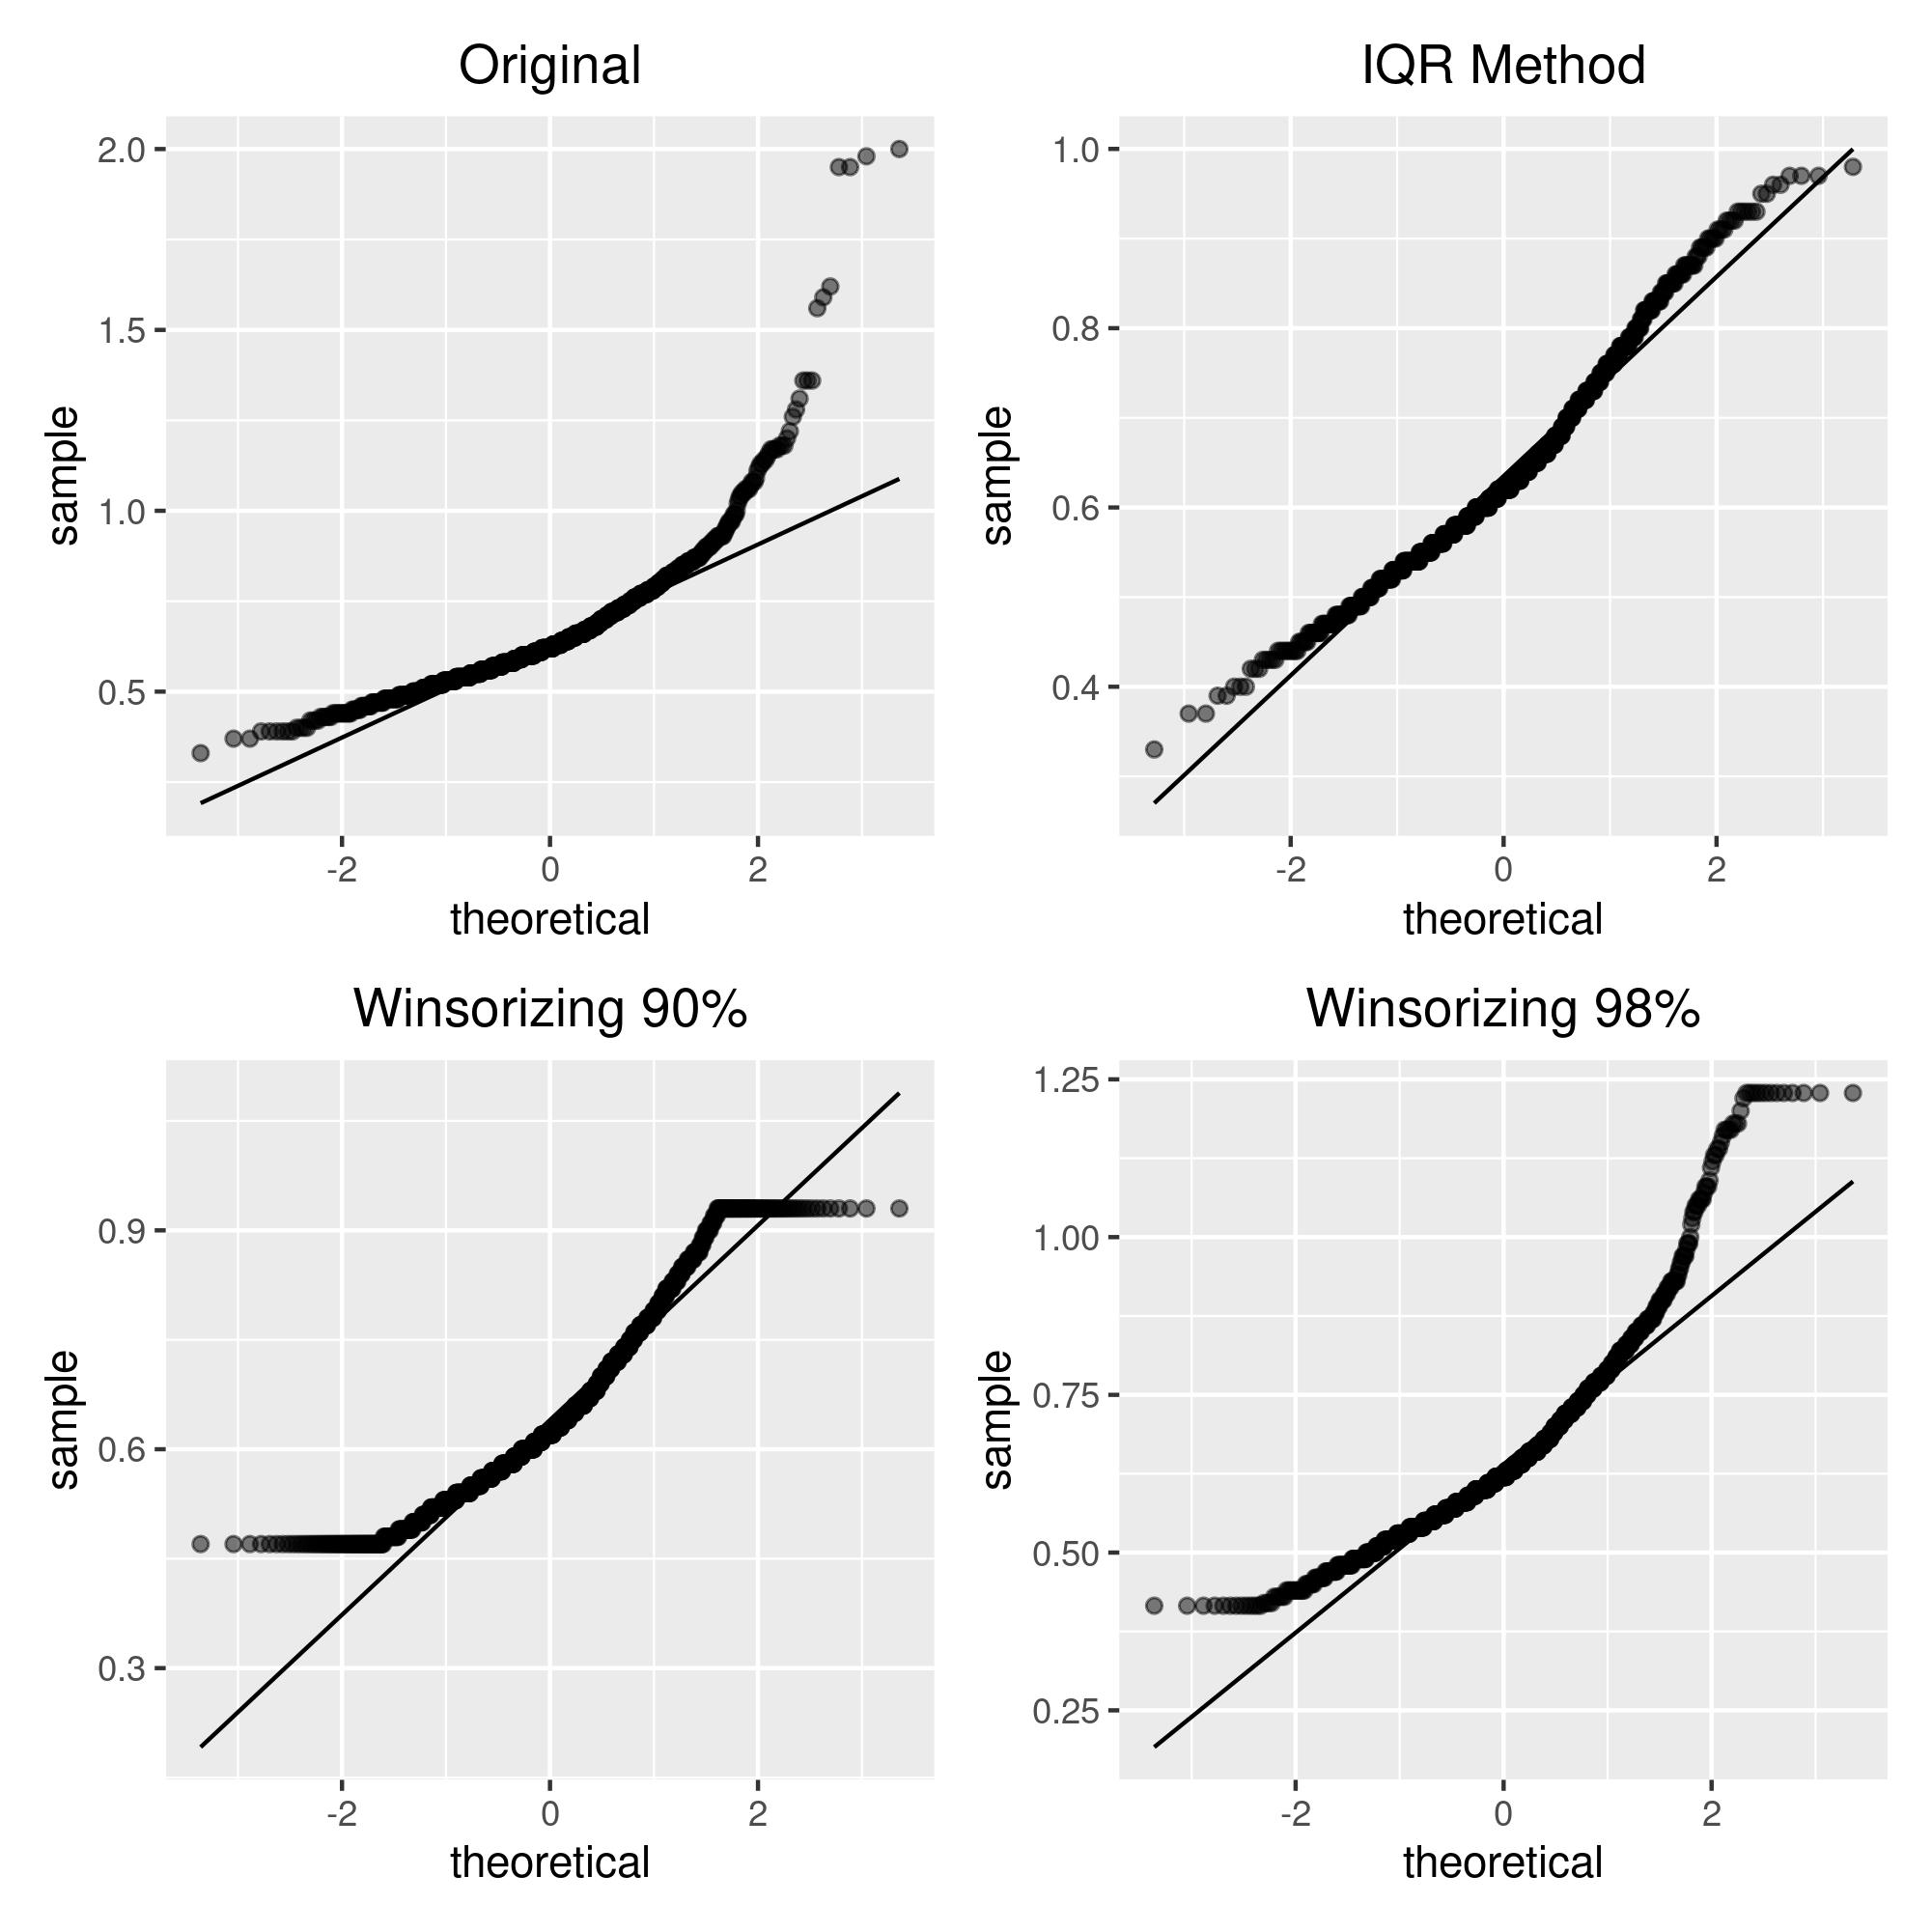
\includegraphics[width=0.45\textwidth]{images/outliers/sulphates_qqplot.png}
    }

    \label{fig:outliers-sulphates}
    \caption{Sulphates}
\end{figure}

\begin{figure}[H]
    \centering

    \subfloat[]{%
        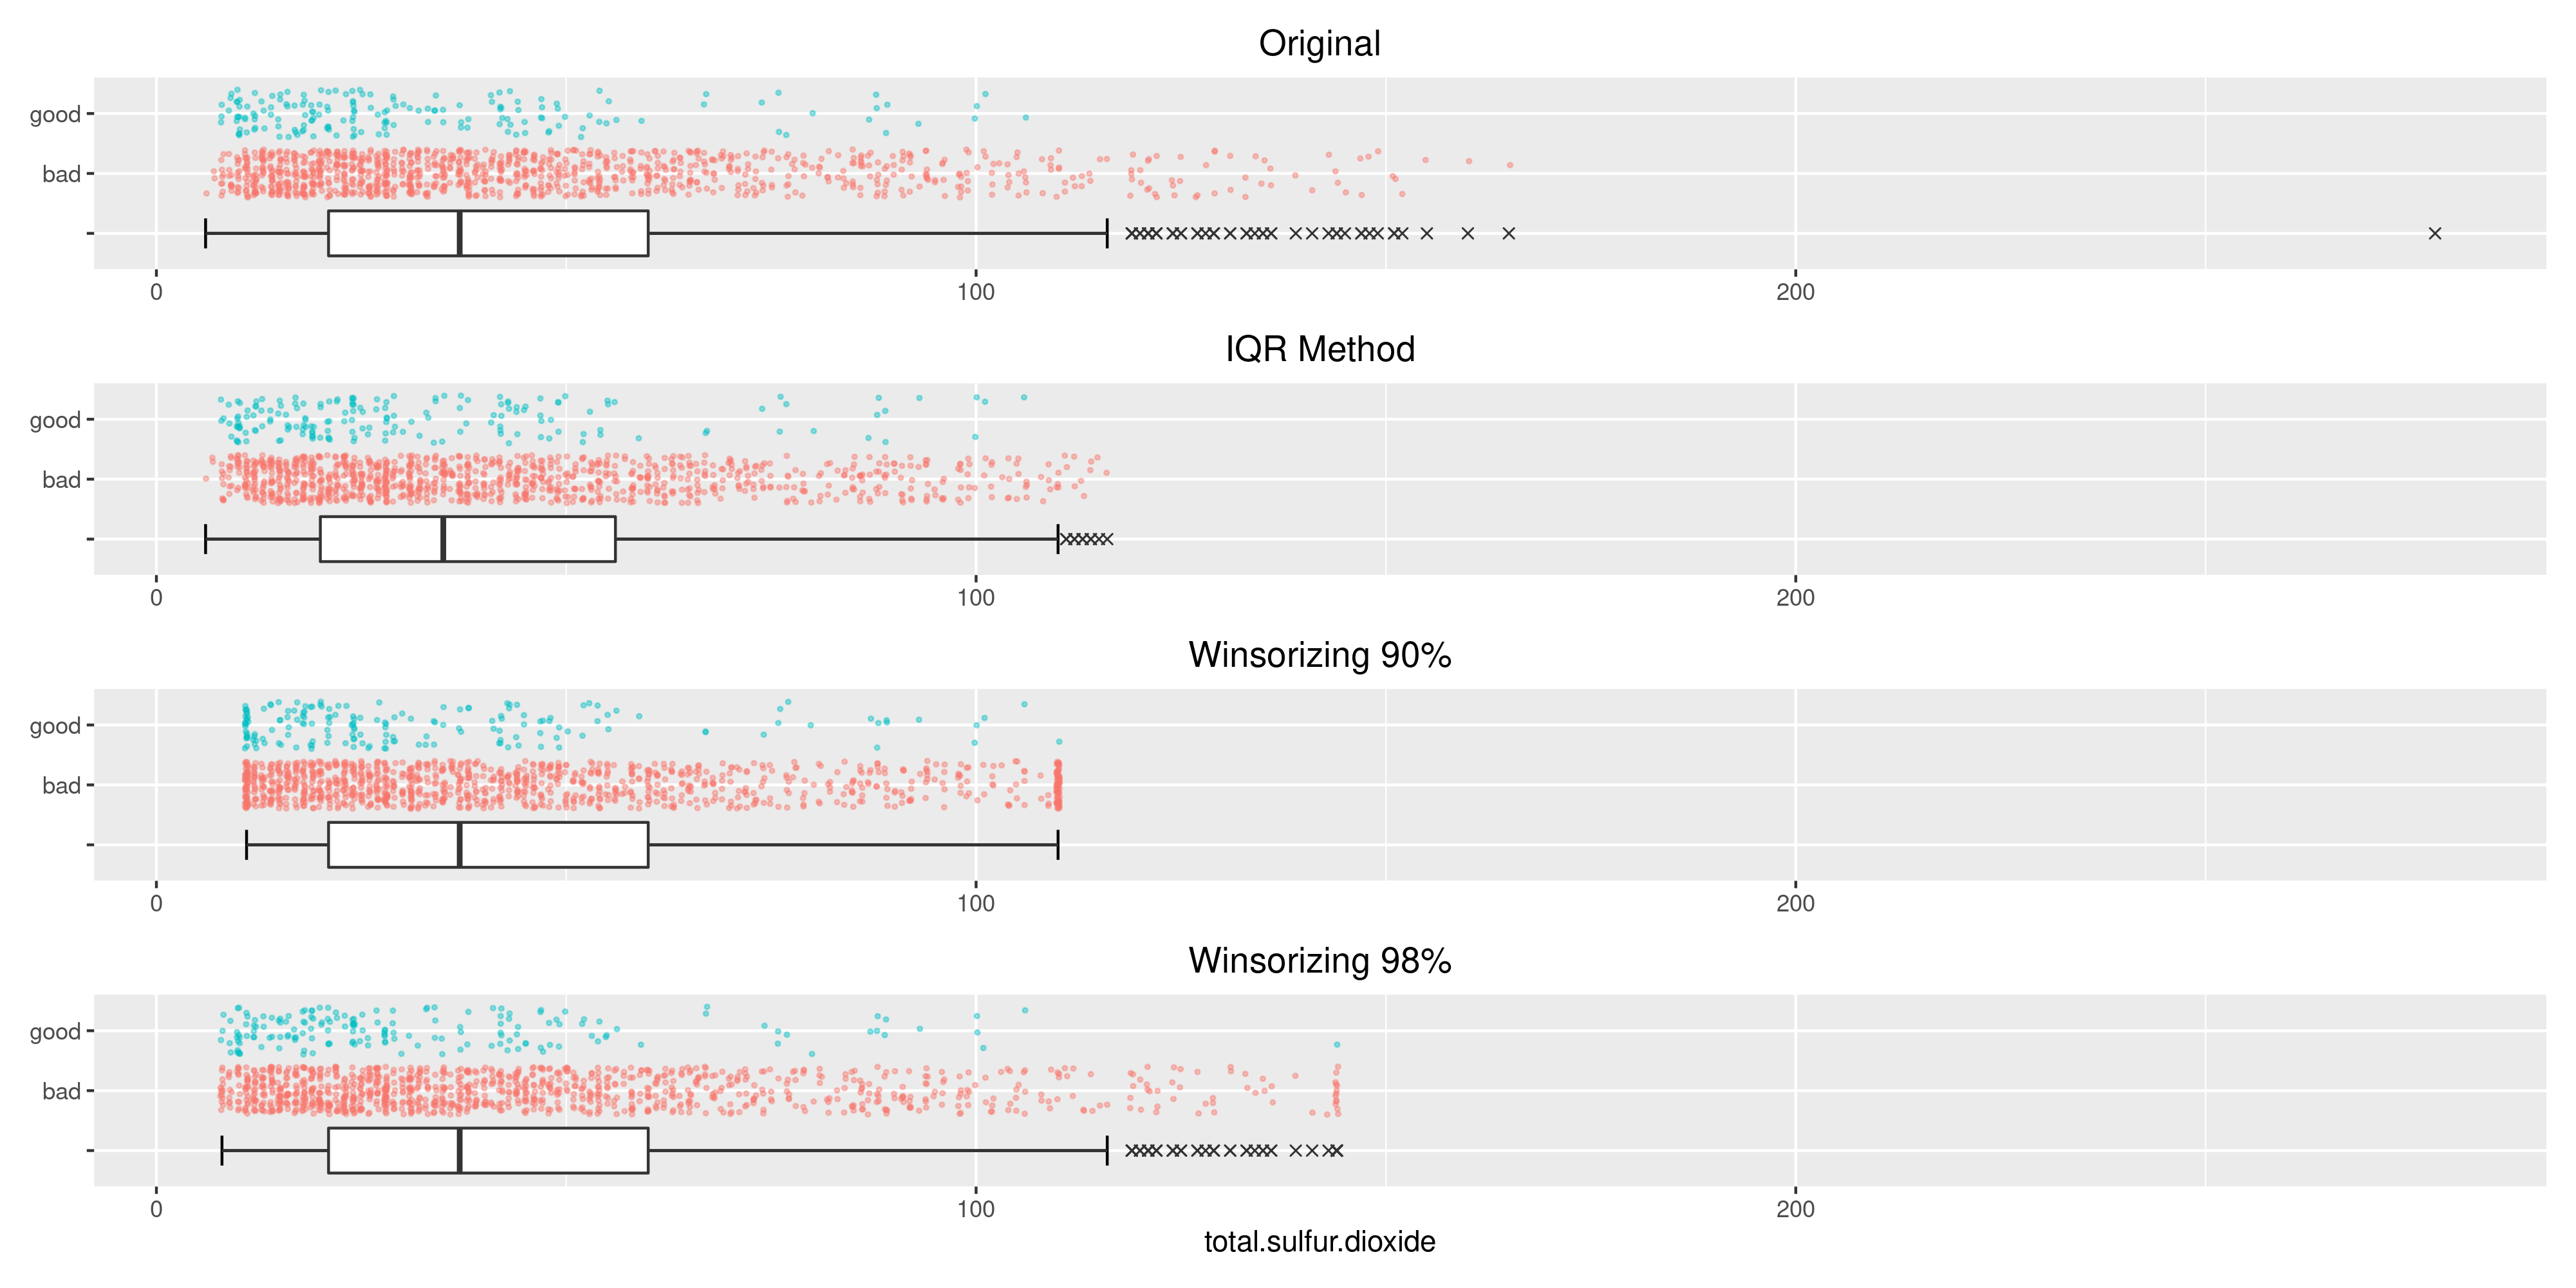
\includegraphics[width=0.99\textwidth]{images/outliers/total.sulfur.dioxide_boxplot.png}
    }

    \subfloat[]{%
        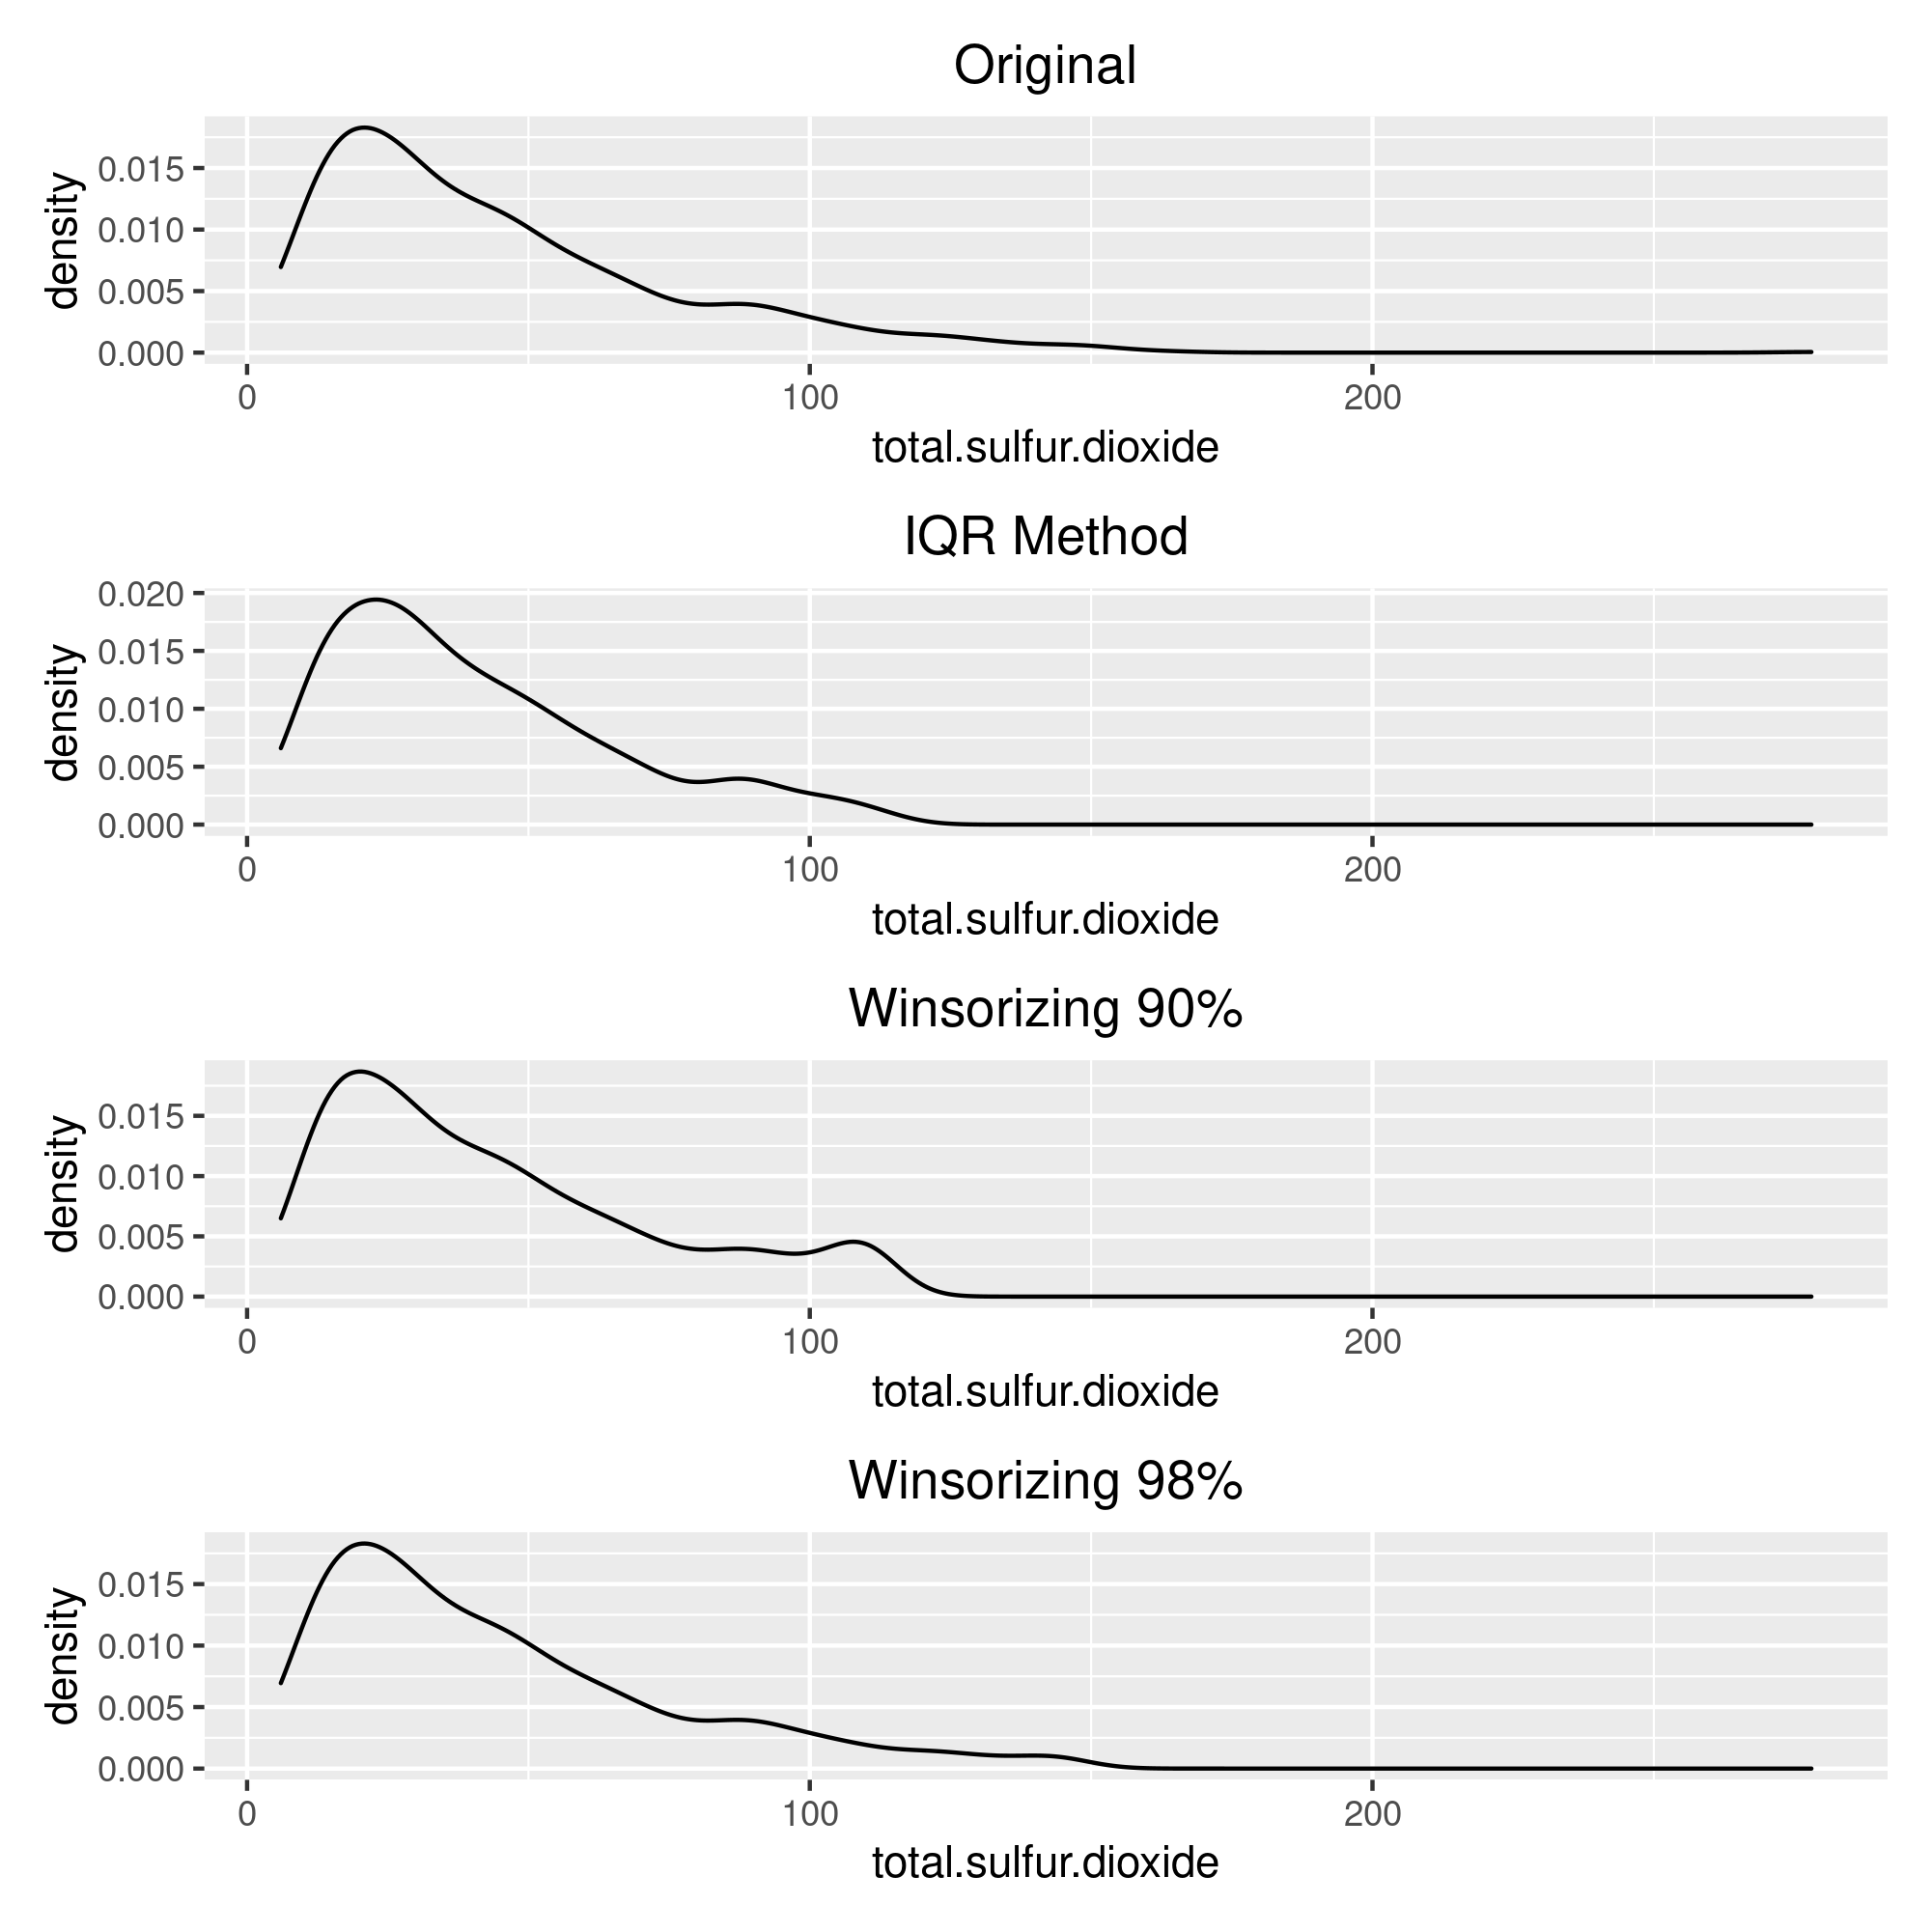
\includegraphics[width=0.45\textwidth]{images/outliers/total.sulfur.dioxide_distribution.png}
    }\qquad
    \subfloat[]{%
        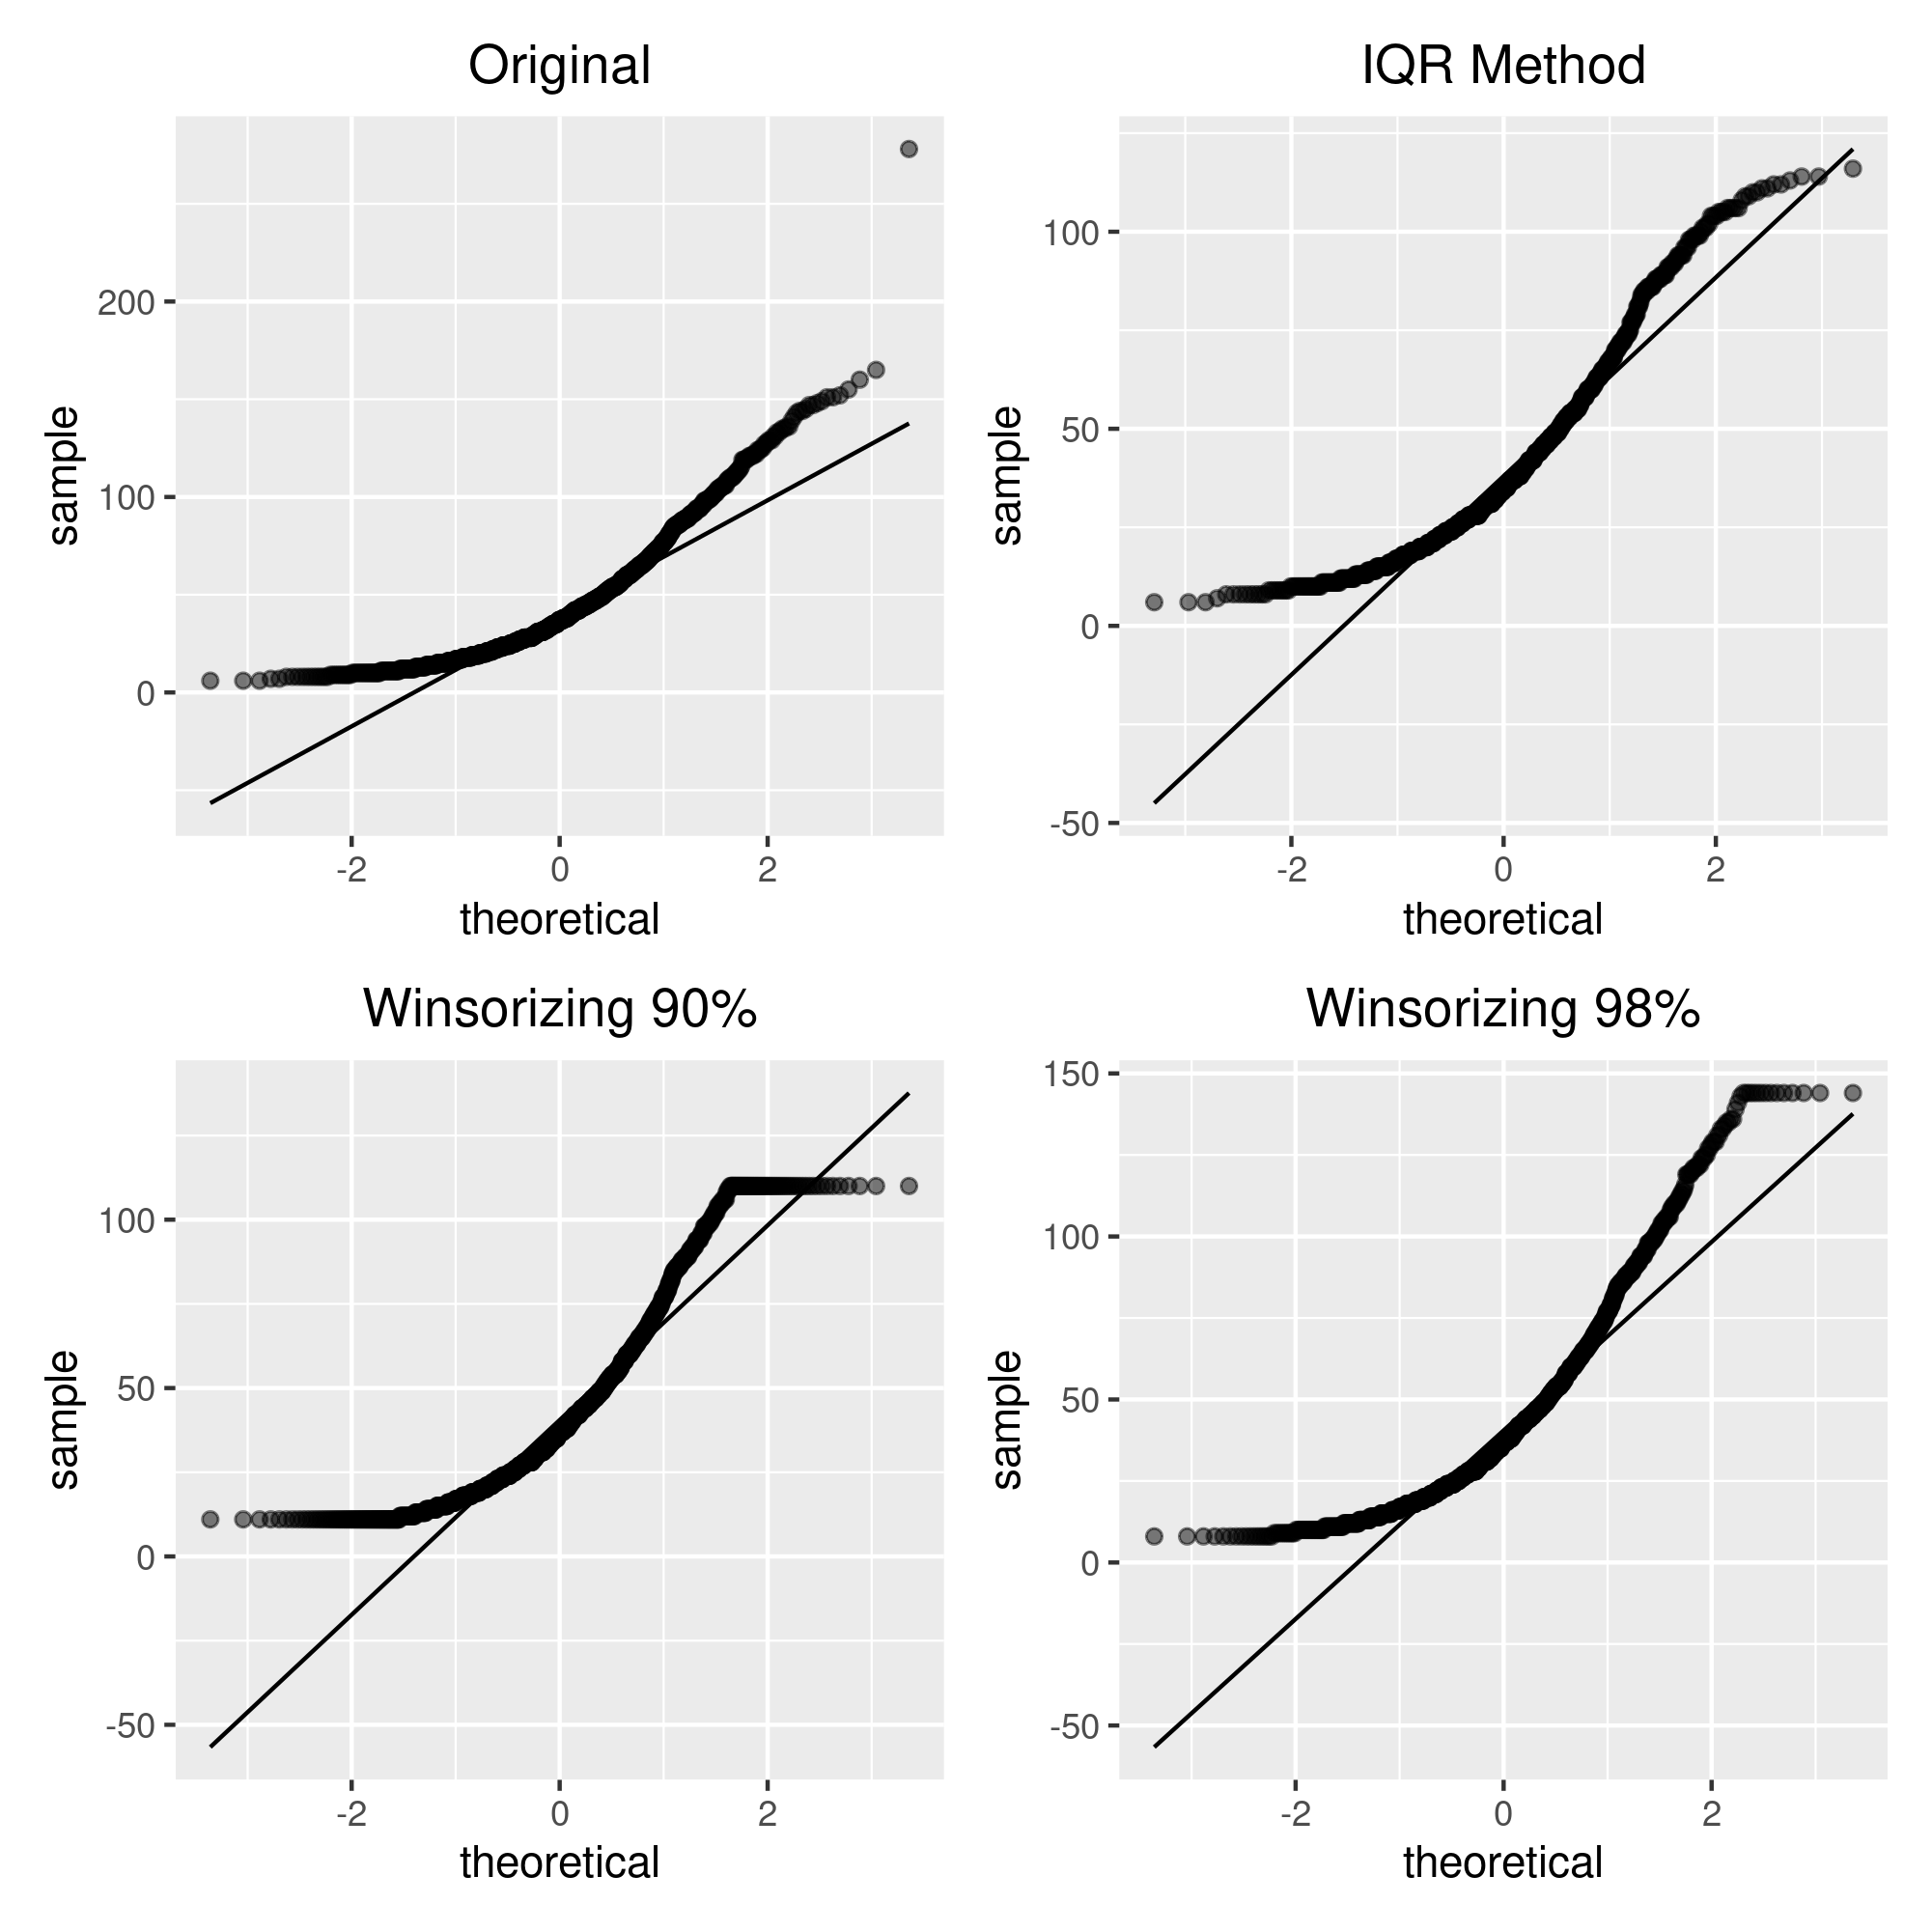
\includegraphics[width=0.45\textwidth]{images/outliers/total.sulfur.dioxide_qqplot.png}
    }

    \label{fig:outliers-total.sulfur.dioxide}
    \caption{Total Sulfur Dioxide}
\end{figure}

\begin{figure}[H]
    \centering

    \subfloat[]{%
        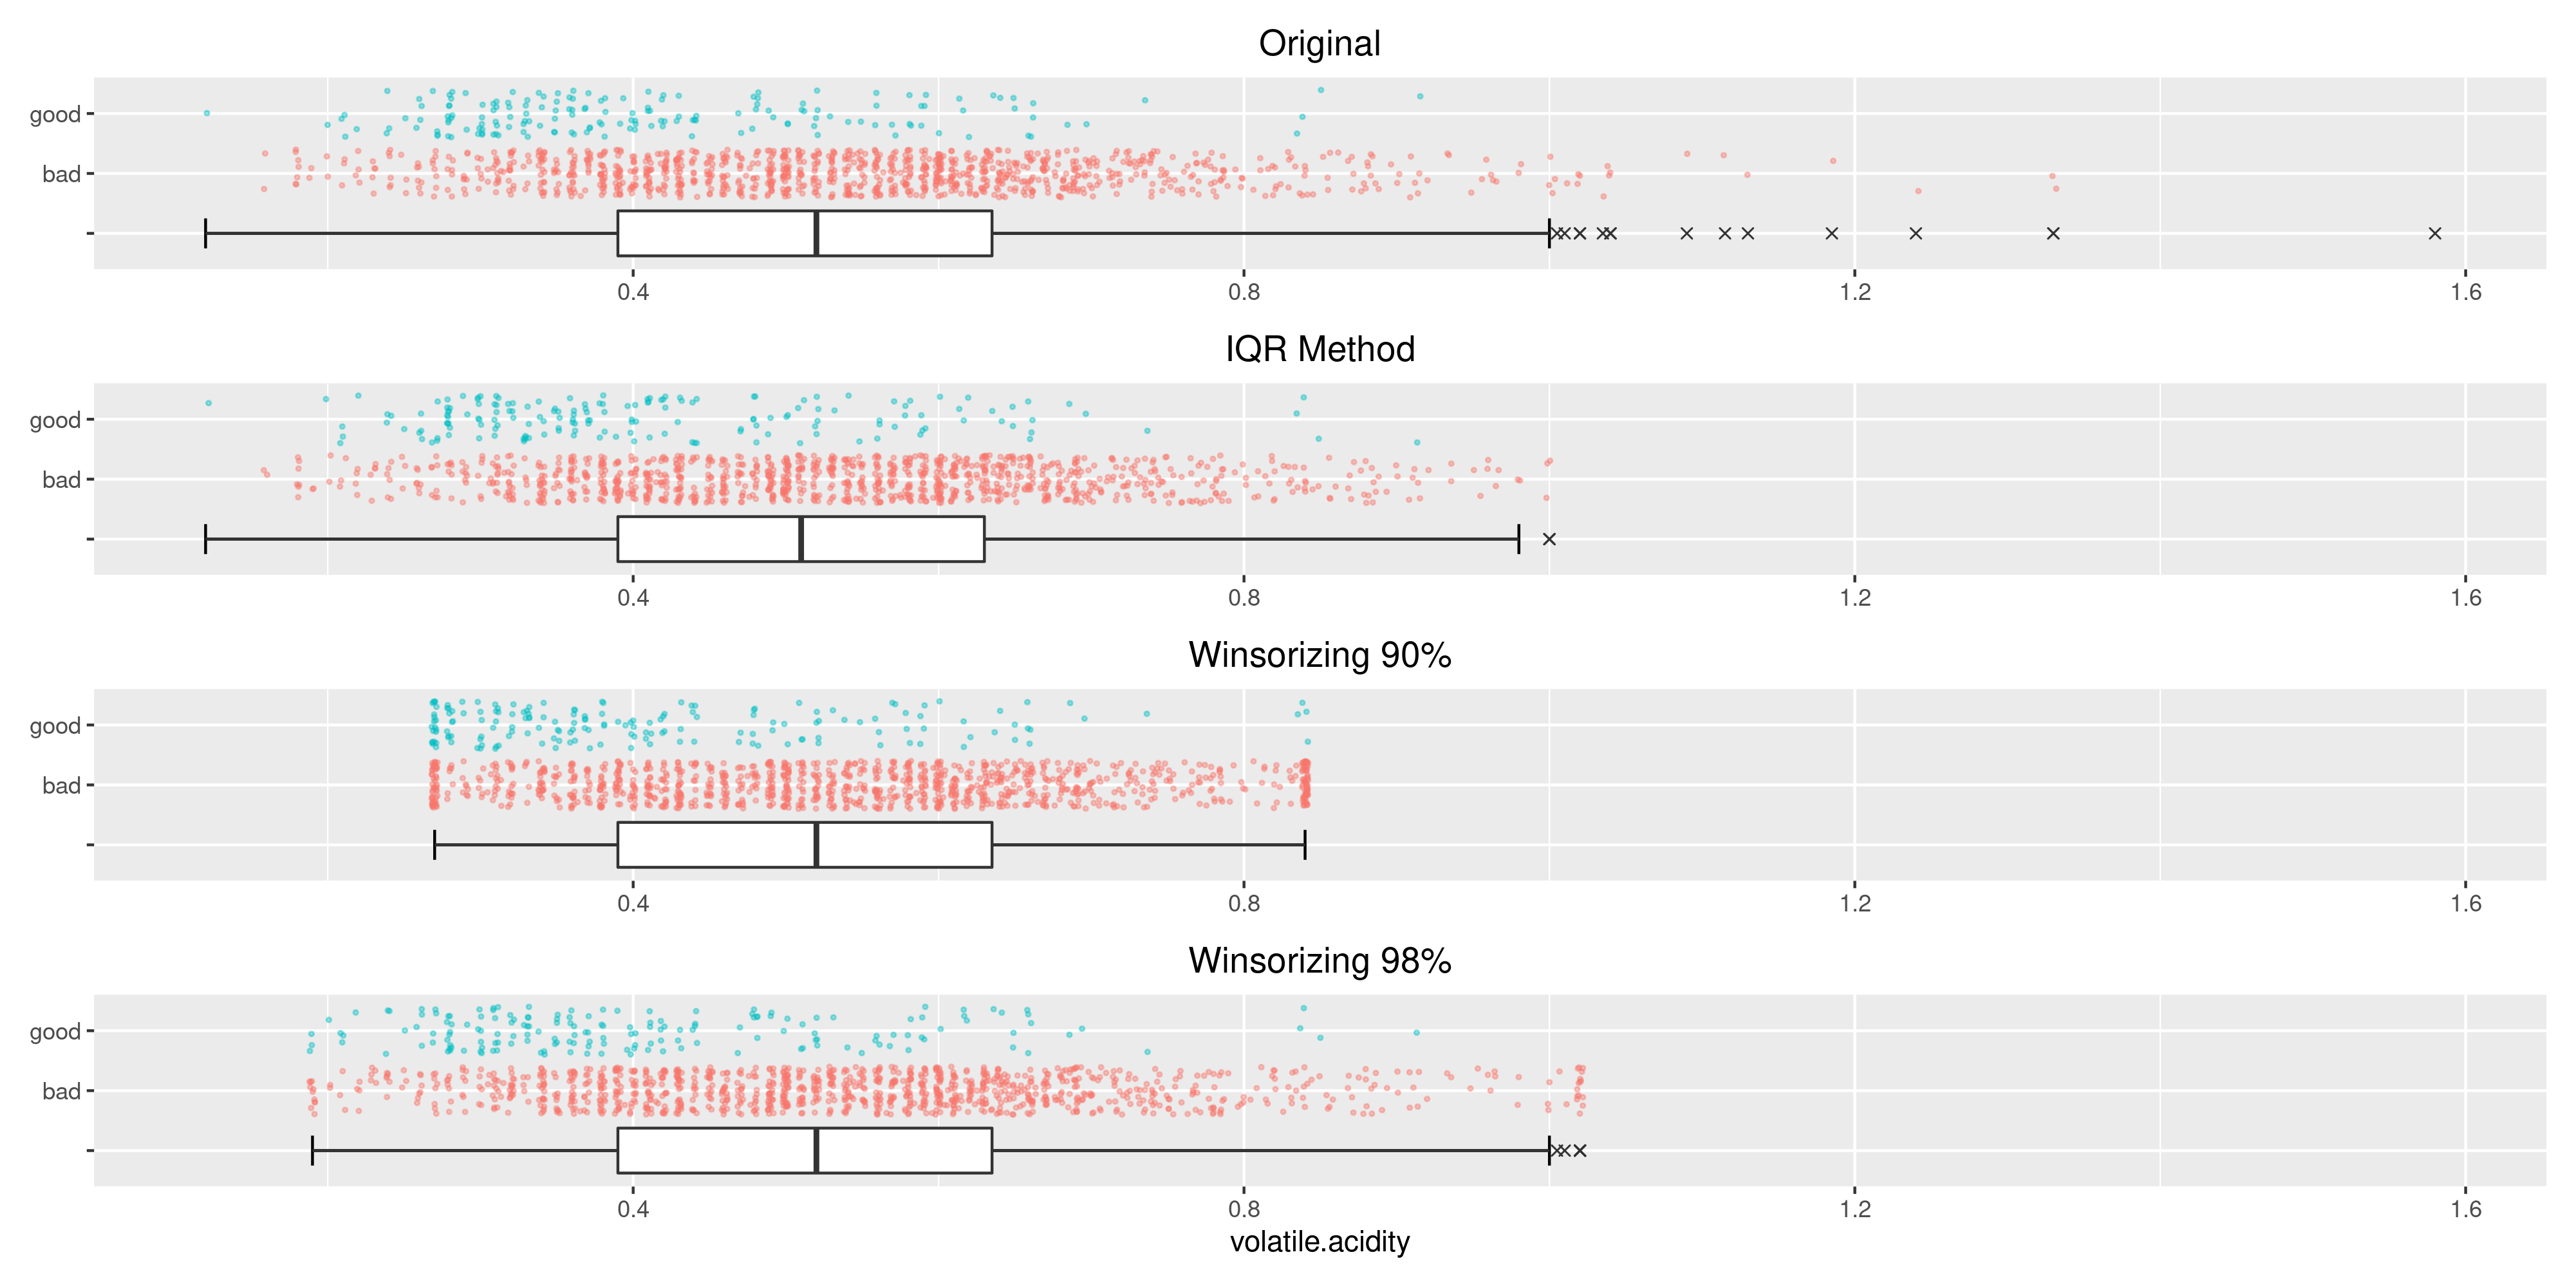
\includegraphics[width=0.99\textwidth]{images/outliers/volatile.acidity_boxplot.png}
    }

    \subfloat[]{%
        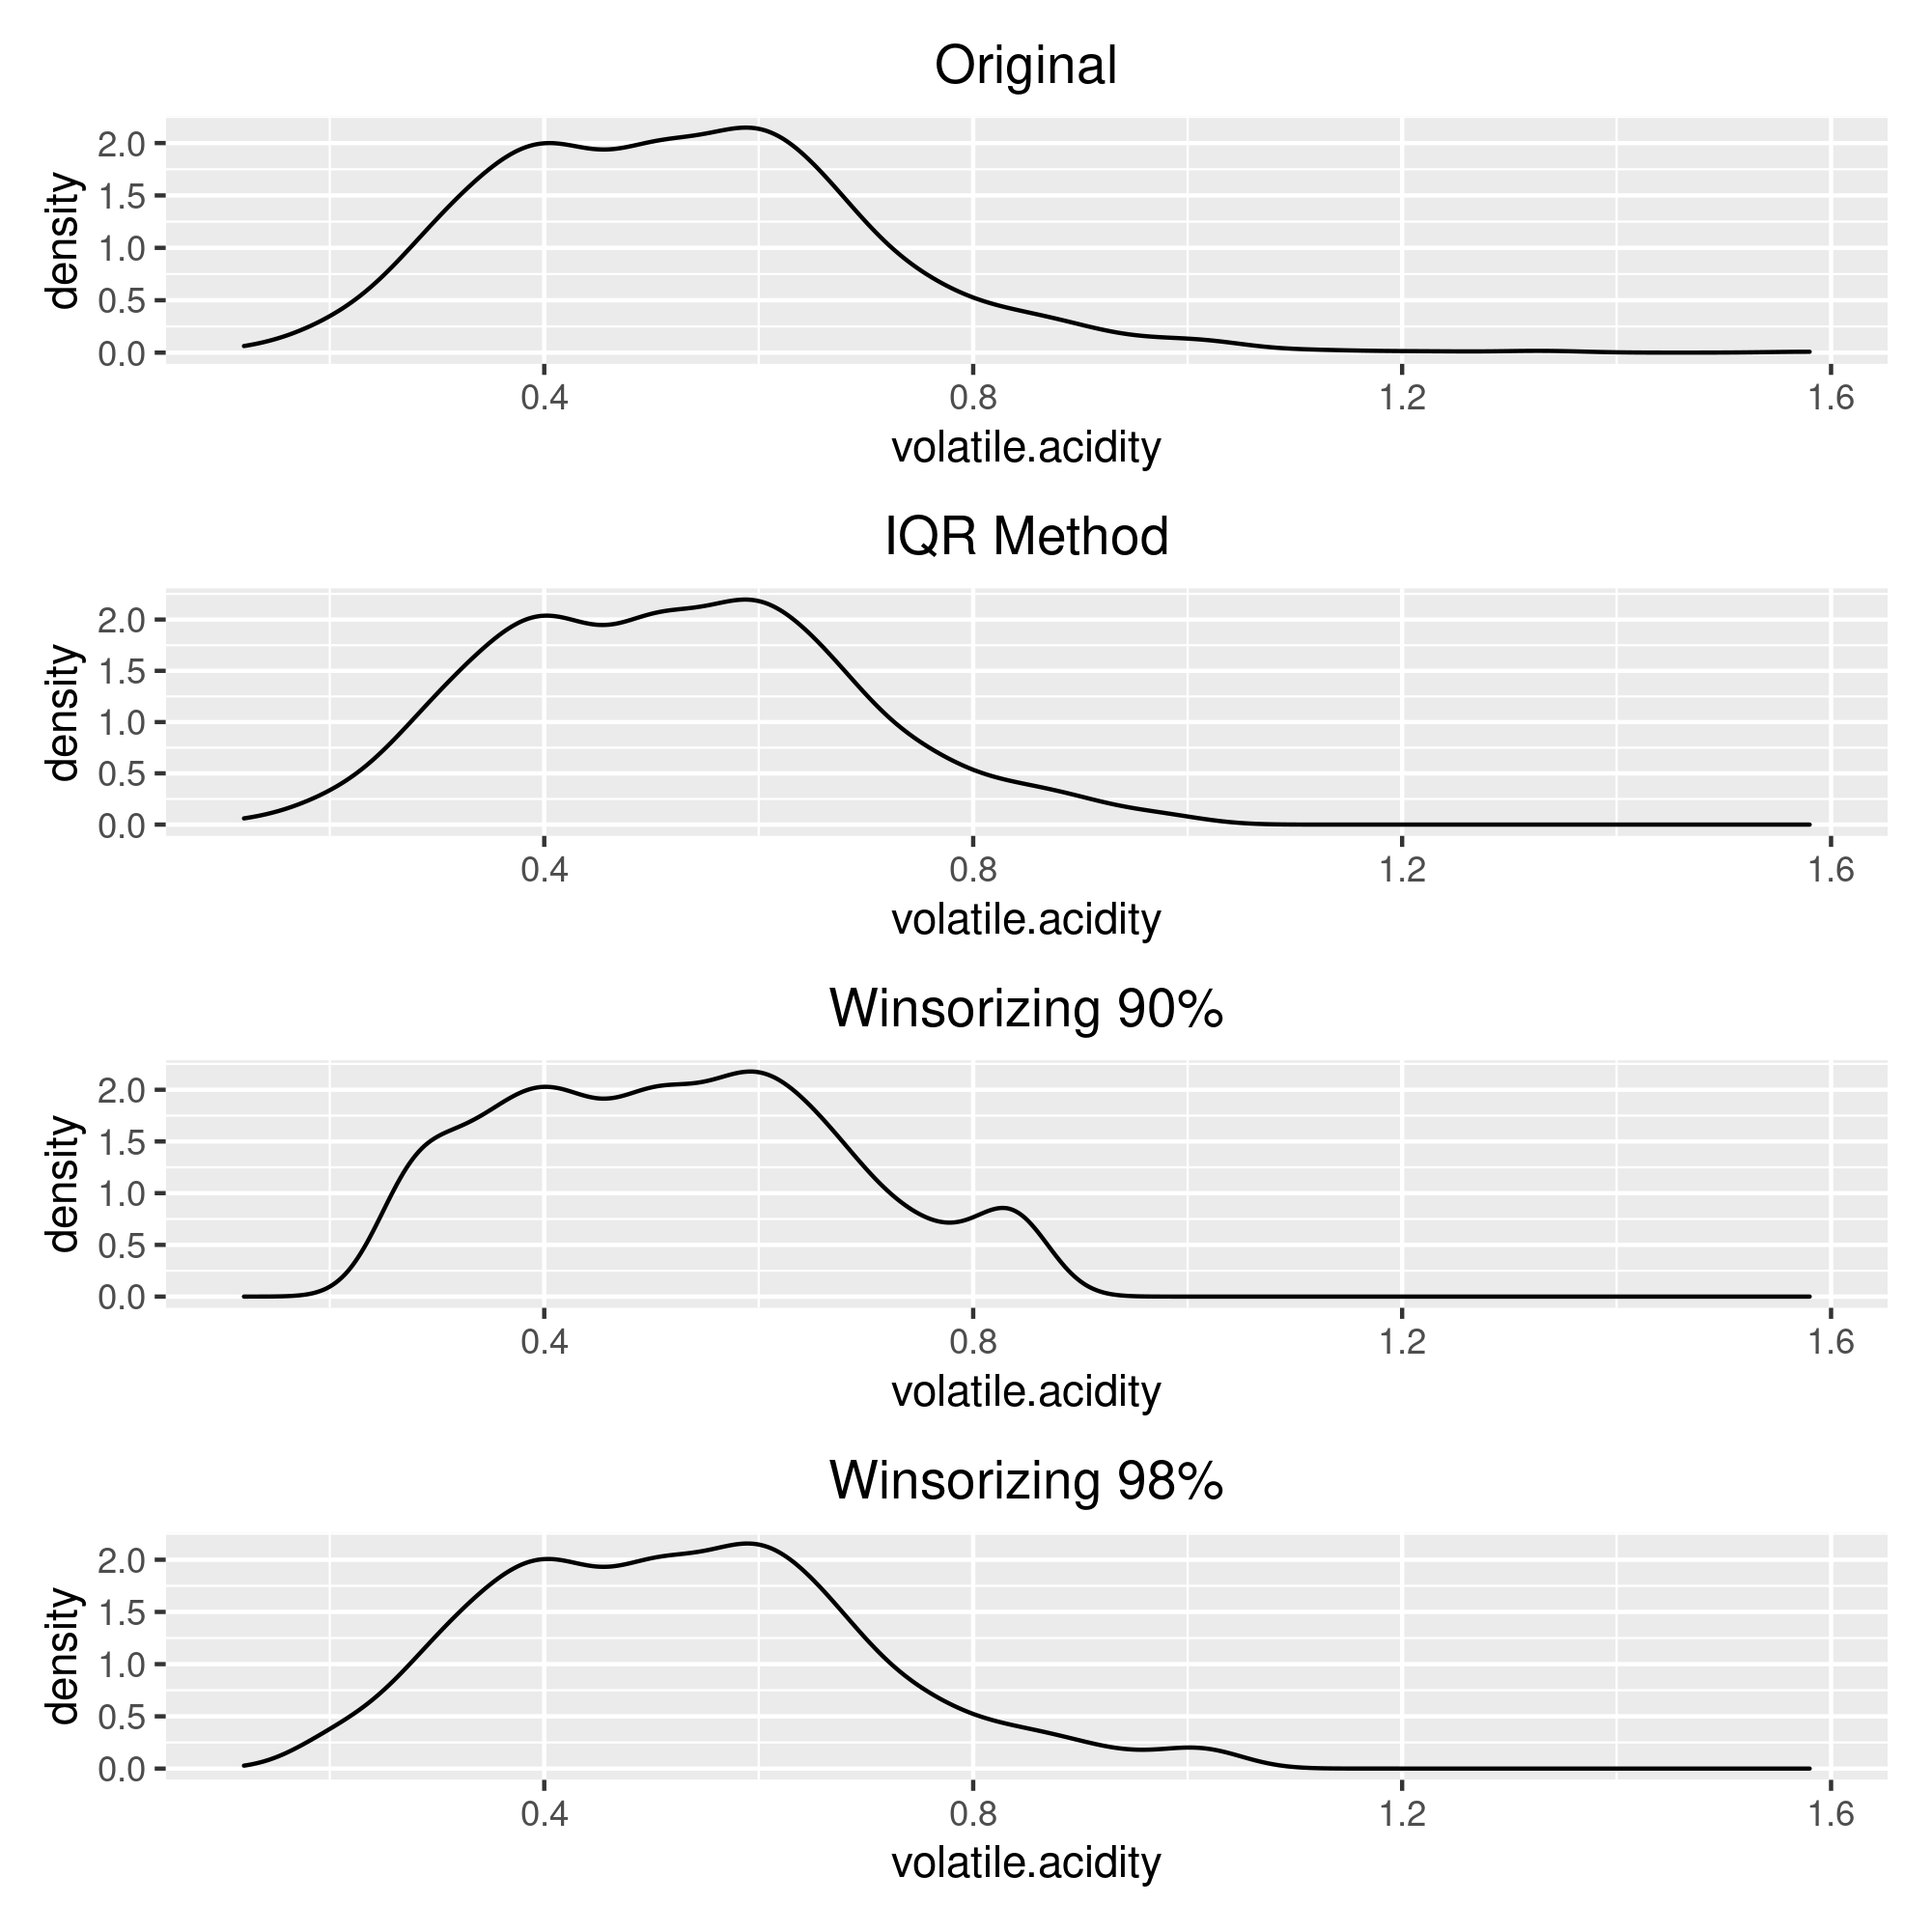
\includegraphics[width=0.45\textwidth]{images/outliers/volatile.acidity_distribution.png}
    }\qquad
    \subfloat[]{%
        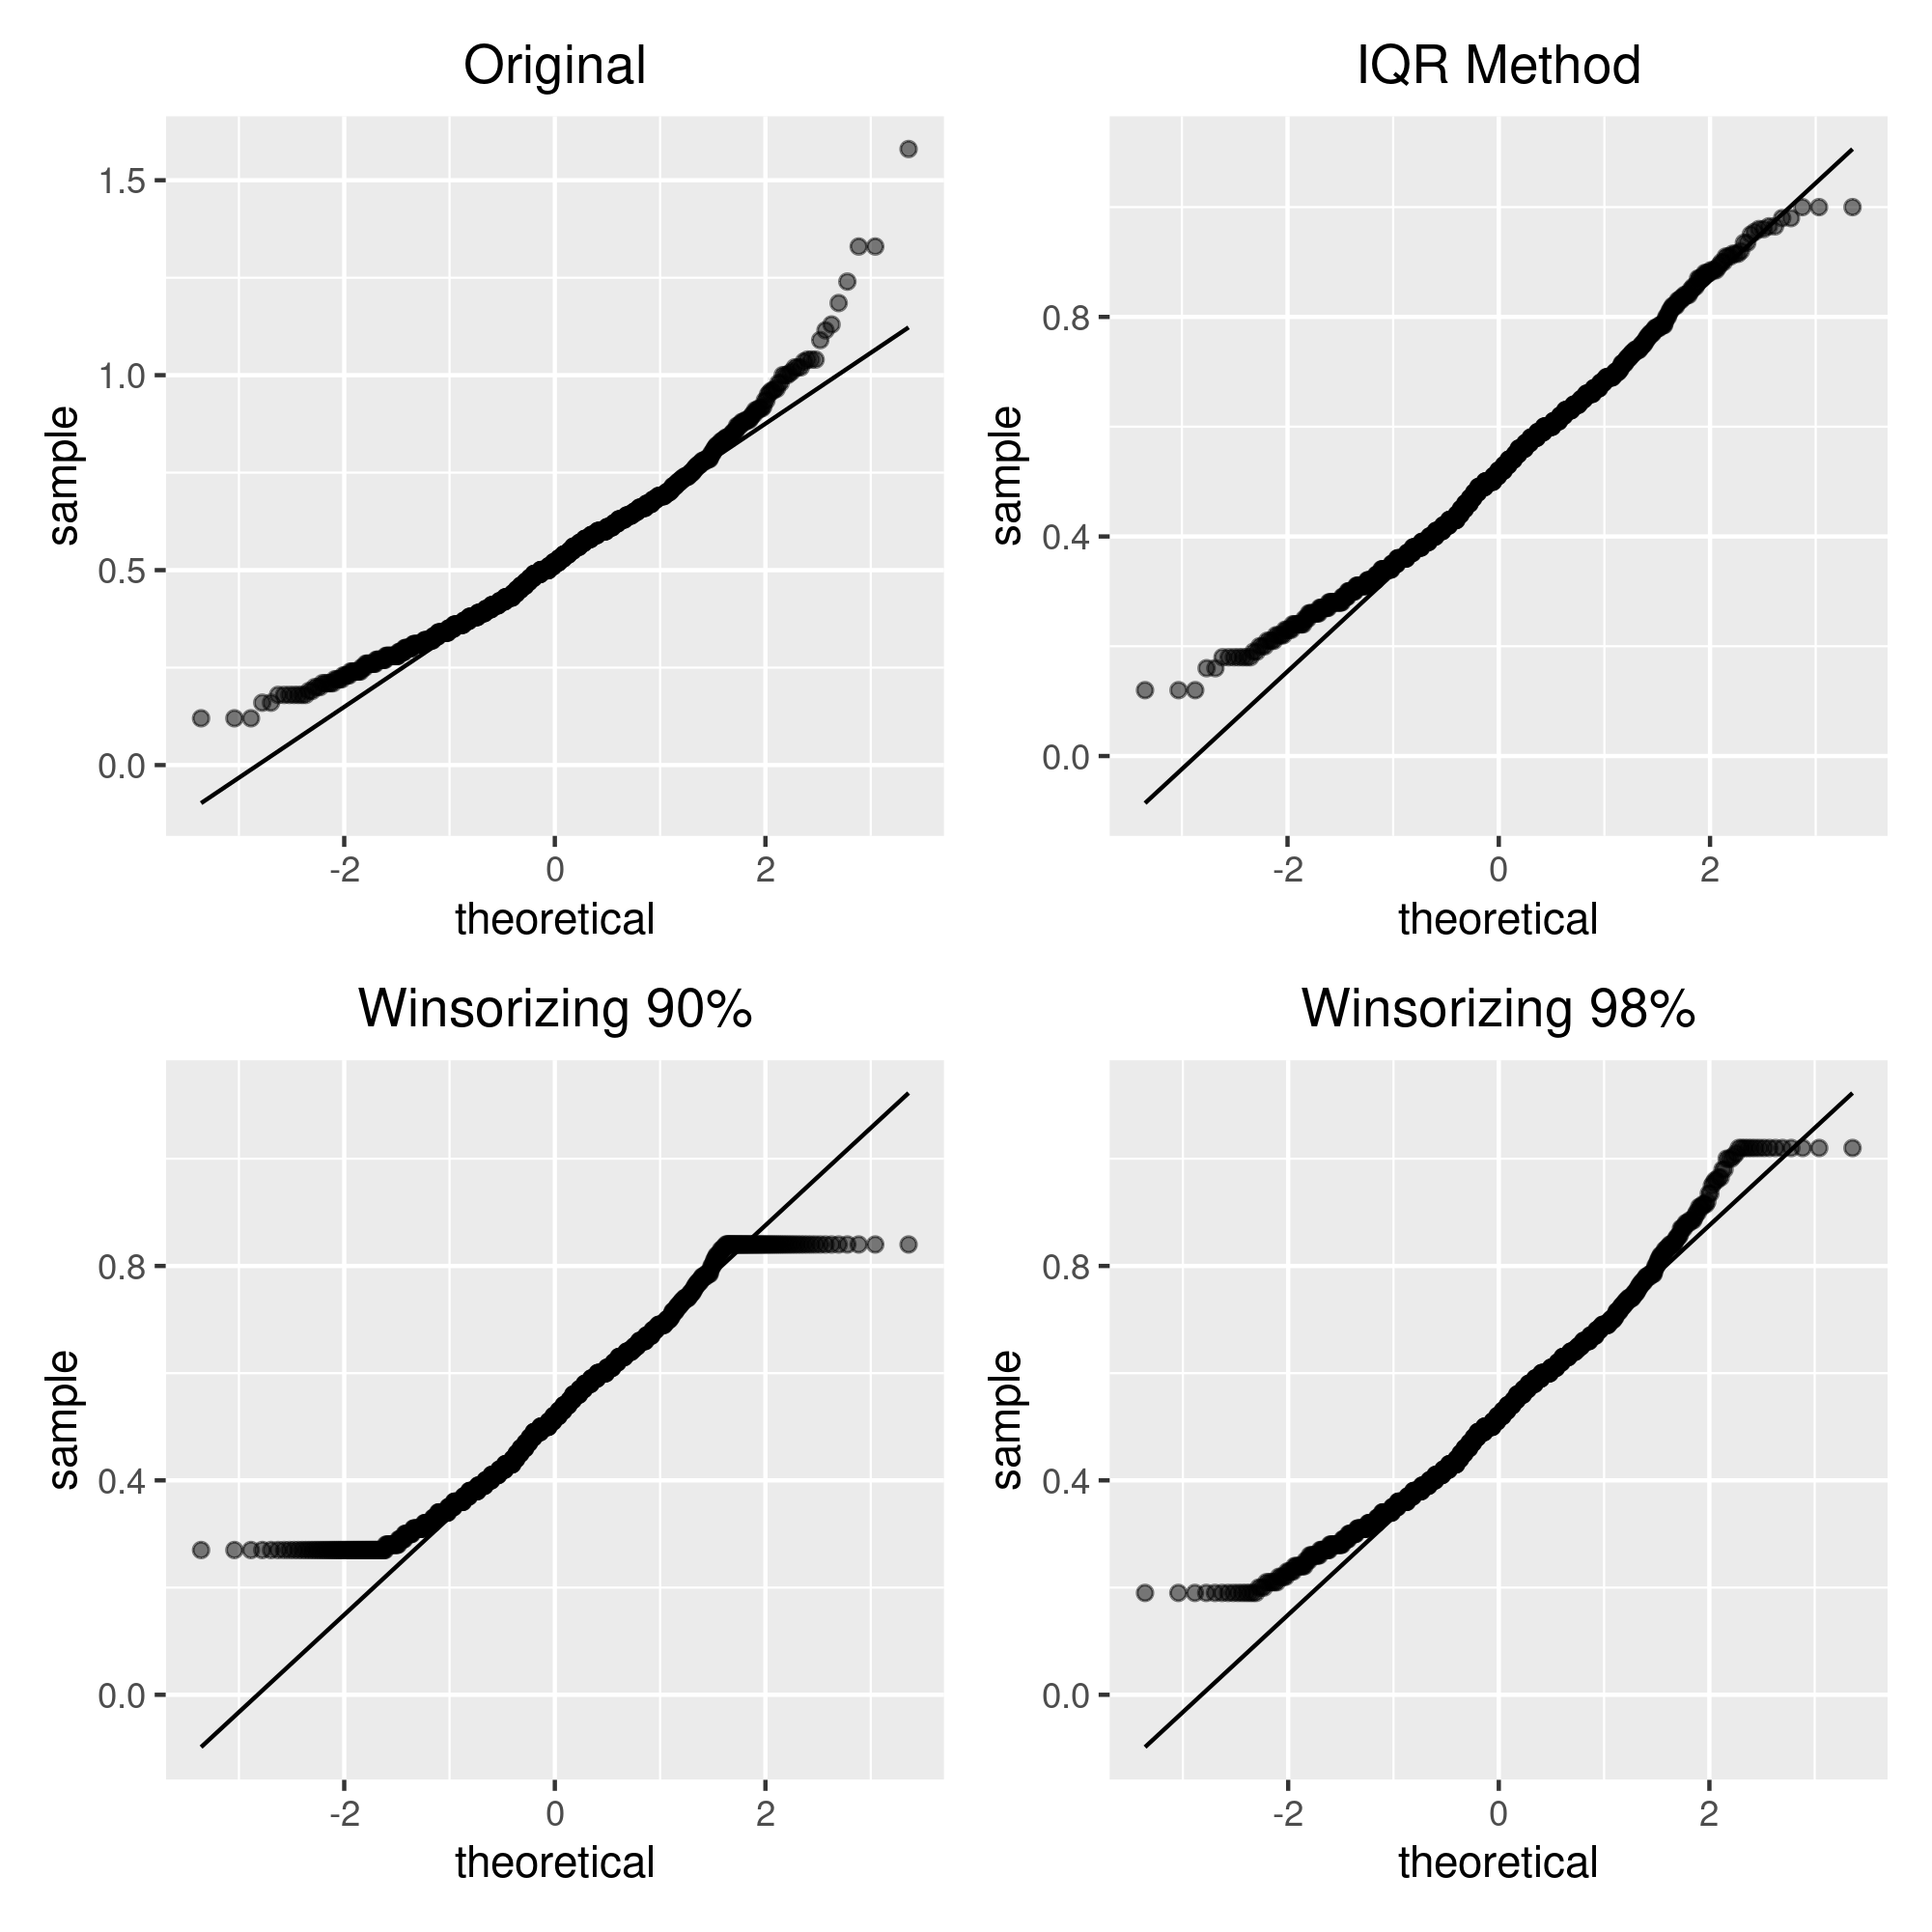
\includegraphics[width=0.45\textwidth]{images/outliers/volatile.acidity_qqplot.png}
    }

    \label{fig:outliers-volatile.acidity}
    \caption{Volatile Acidity}
\end{figure}

\newpage
